\chapter[Control regions for fakes][Control regions for fakes]{Control regions for fakes}
\label{apx:control-regions}

\begin{quote}
Comparisons of data with prediction for fakes control regions in the $\Htautau$ analysis are shown.
\end{quote}

\section{Same sign CR}

\begin{figure}[tp]
  \centering
  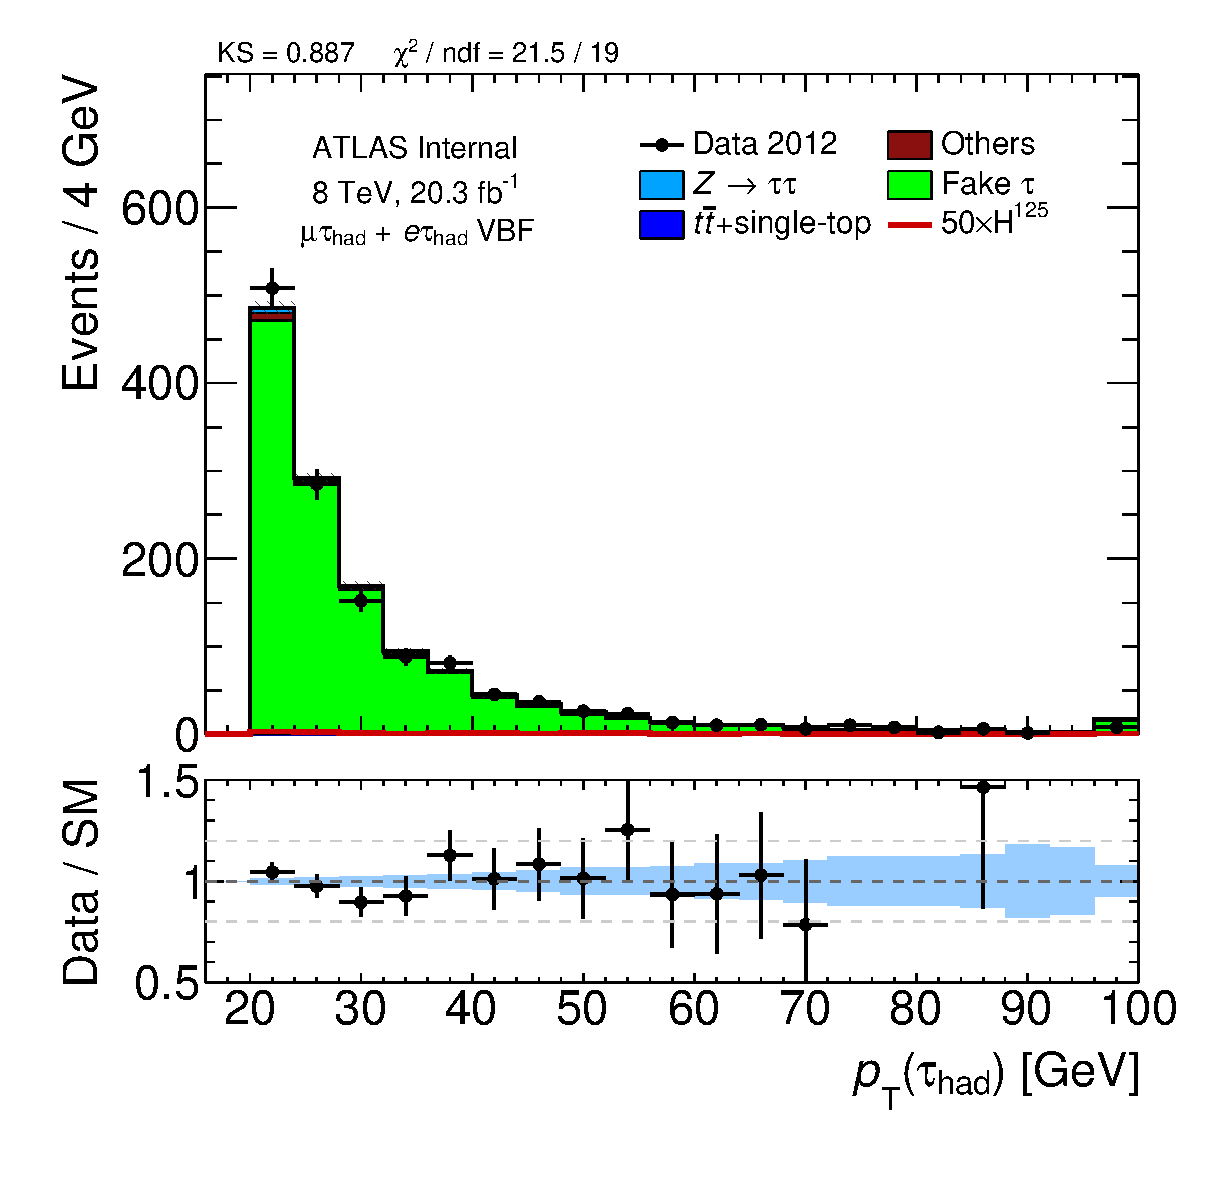
\includegraphics[width=0.32\textwidth]{figures/analysis/vbf-SSXCR/tau-pt}
  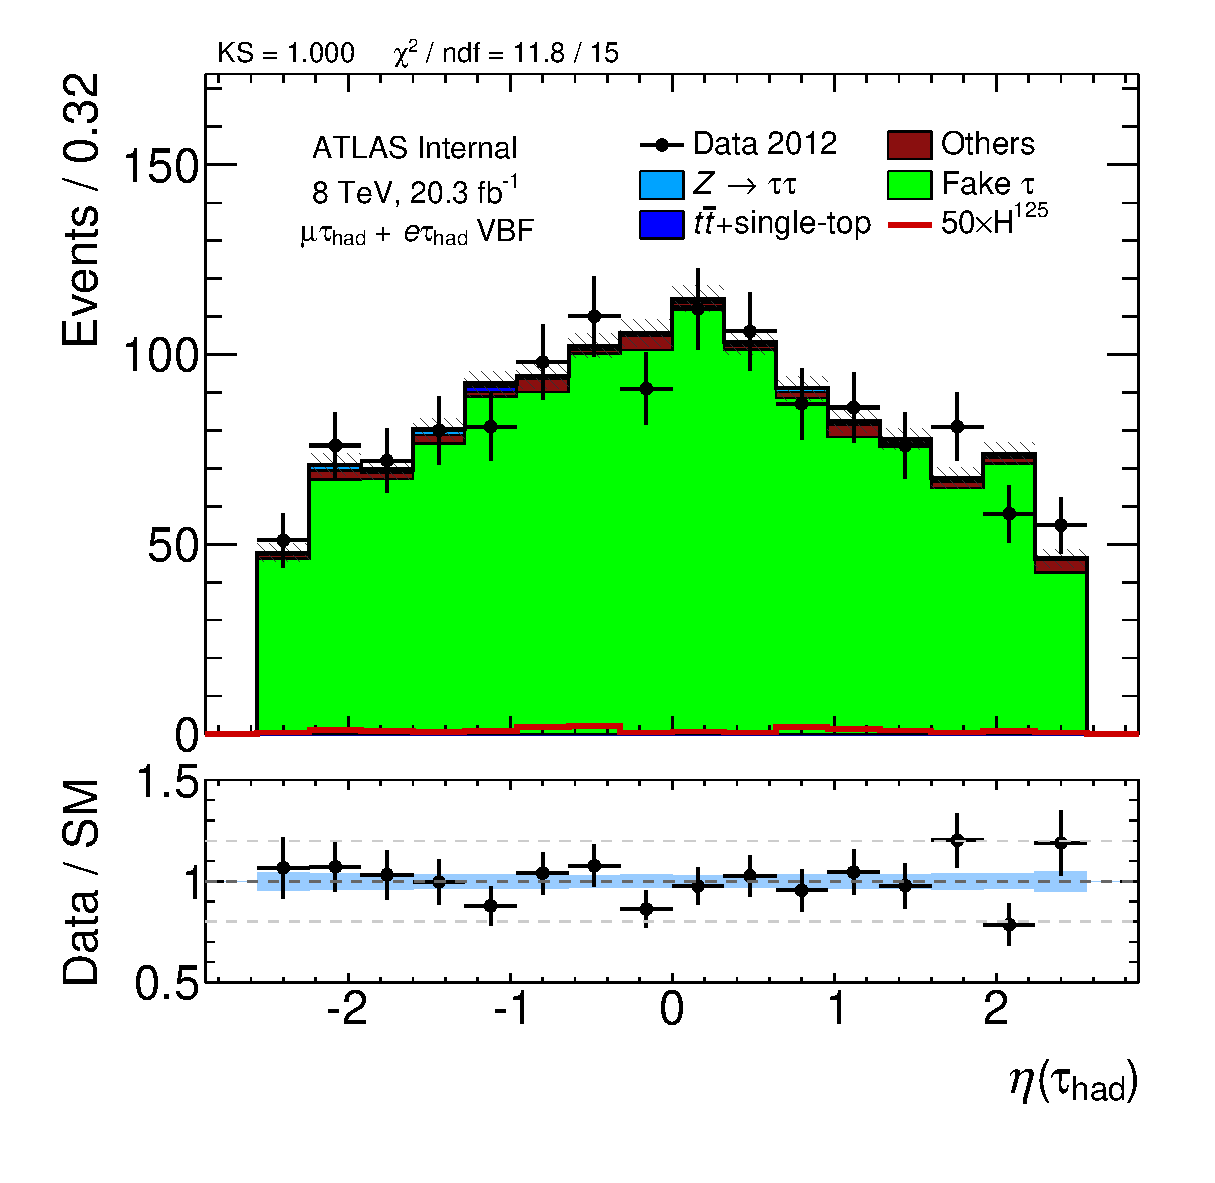
\includegraphics[width=0.32\textwidth]{figures/analysis/vbf-SSXCR/tau-eta}
  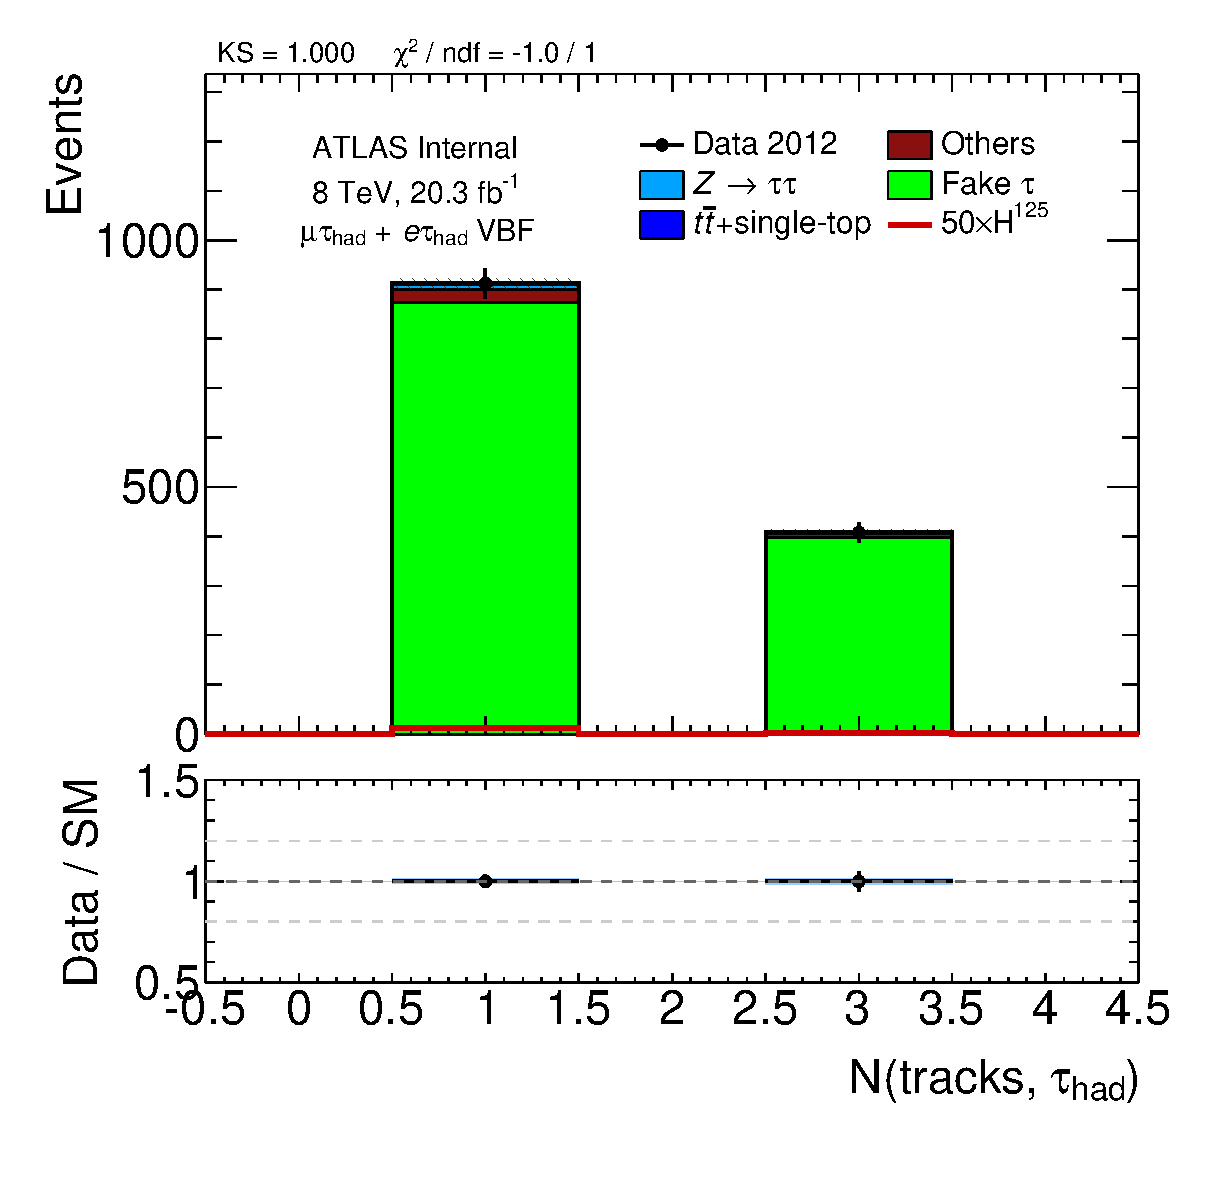
\includegraphics[width=0.32\textwidth]{figures/analysis/vbf-SSXCR/tau-numTrack} \\
  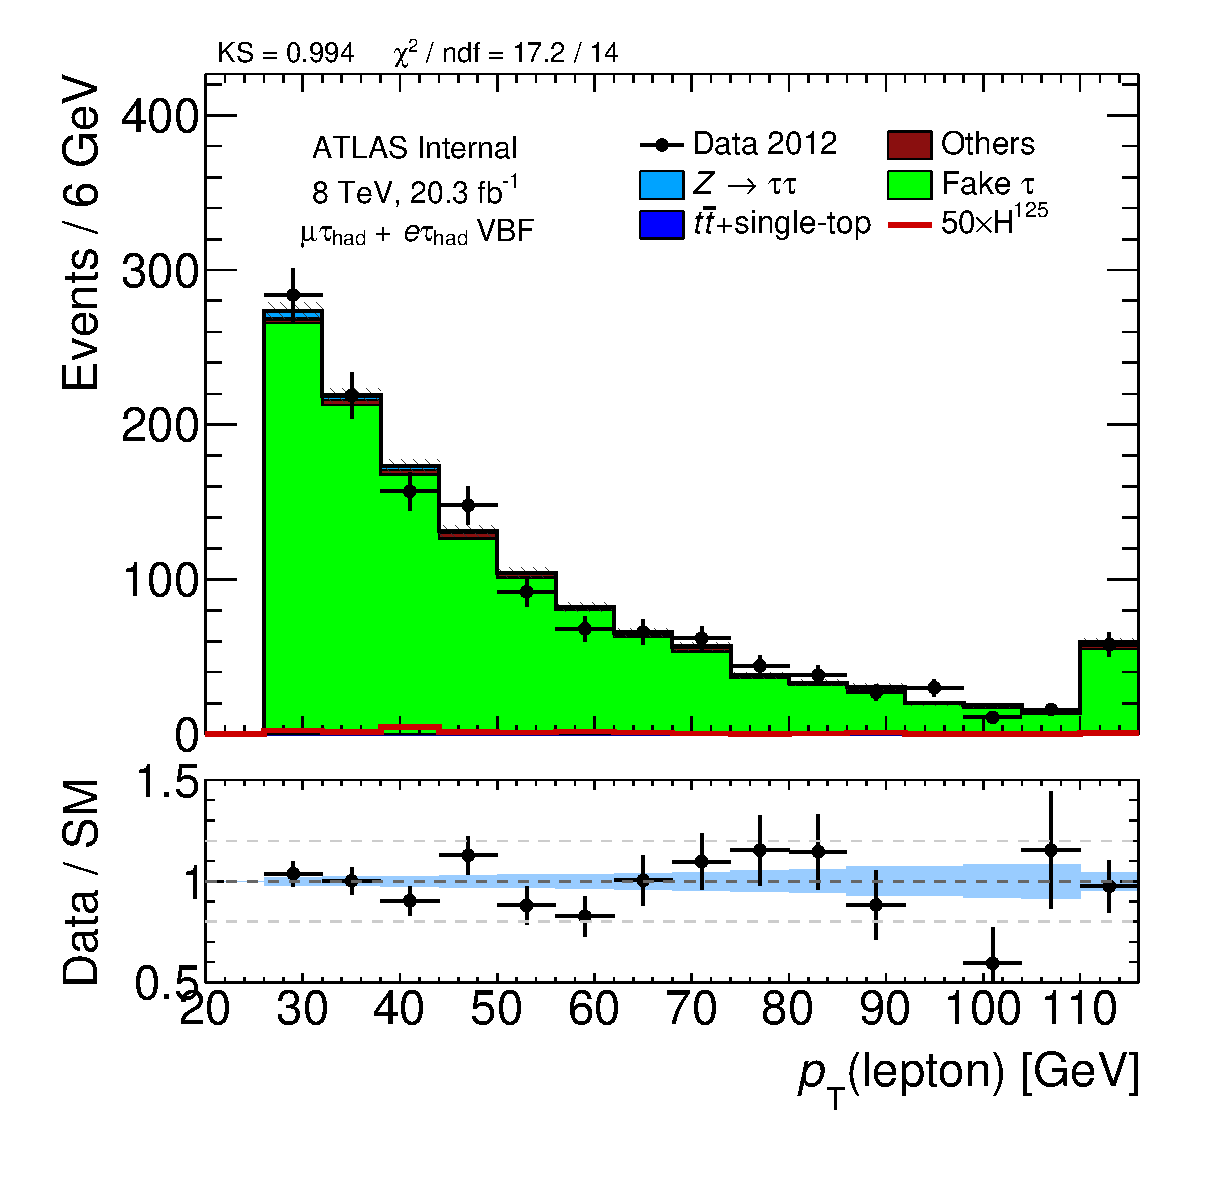
\includegraphics[width=0.32\textwidth]{figures/analysis/vbf-SSXCR/lep-pt-hi}
  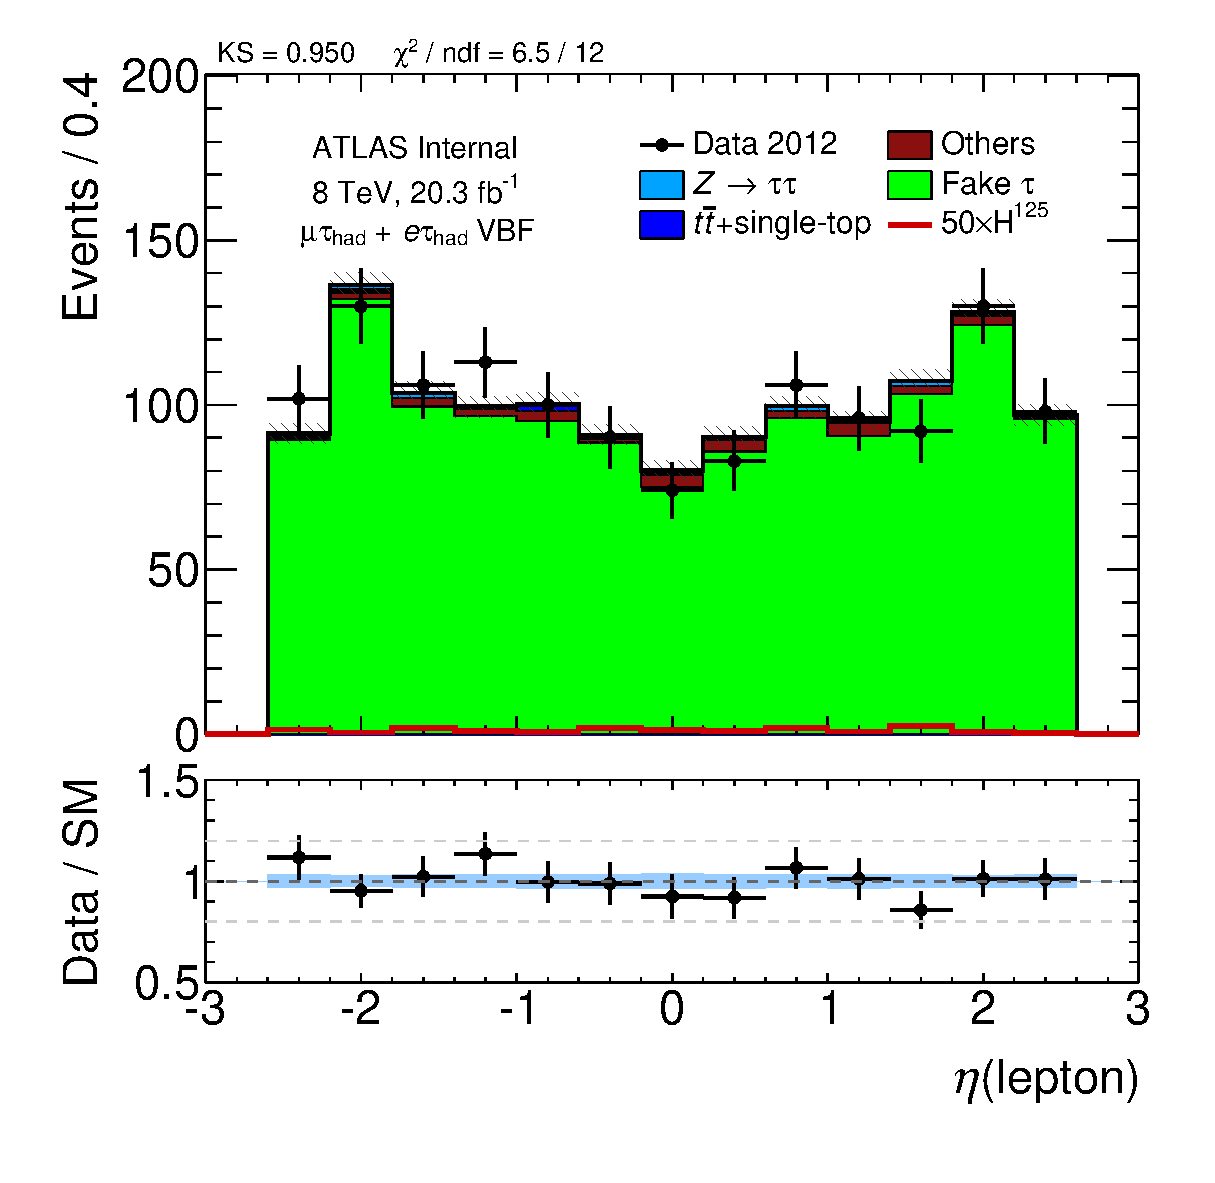
\includegraphics[width=0.32\textwidth]{figures/analysis/vbf-SSXCR/lep-eta}
  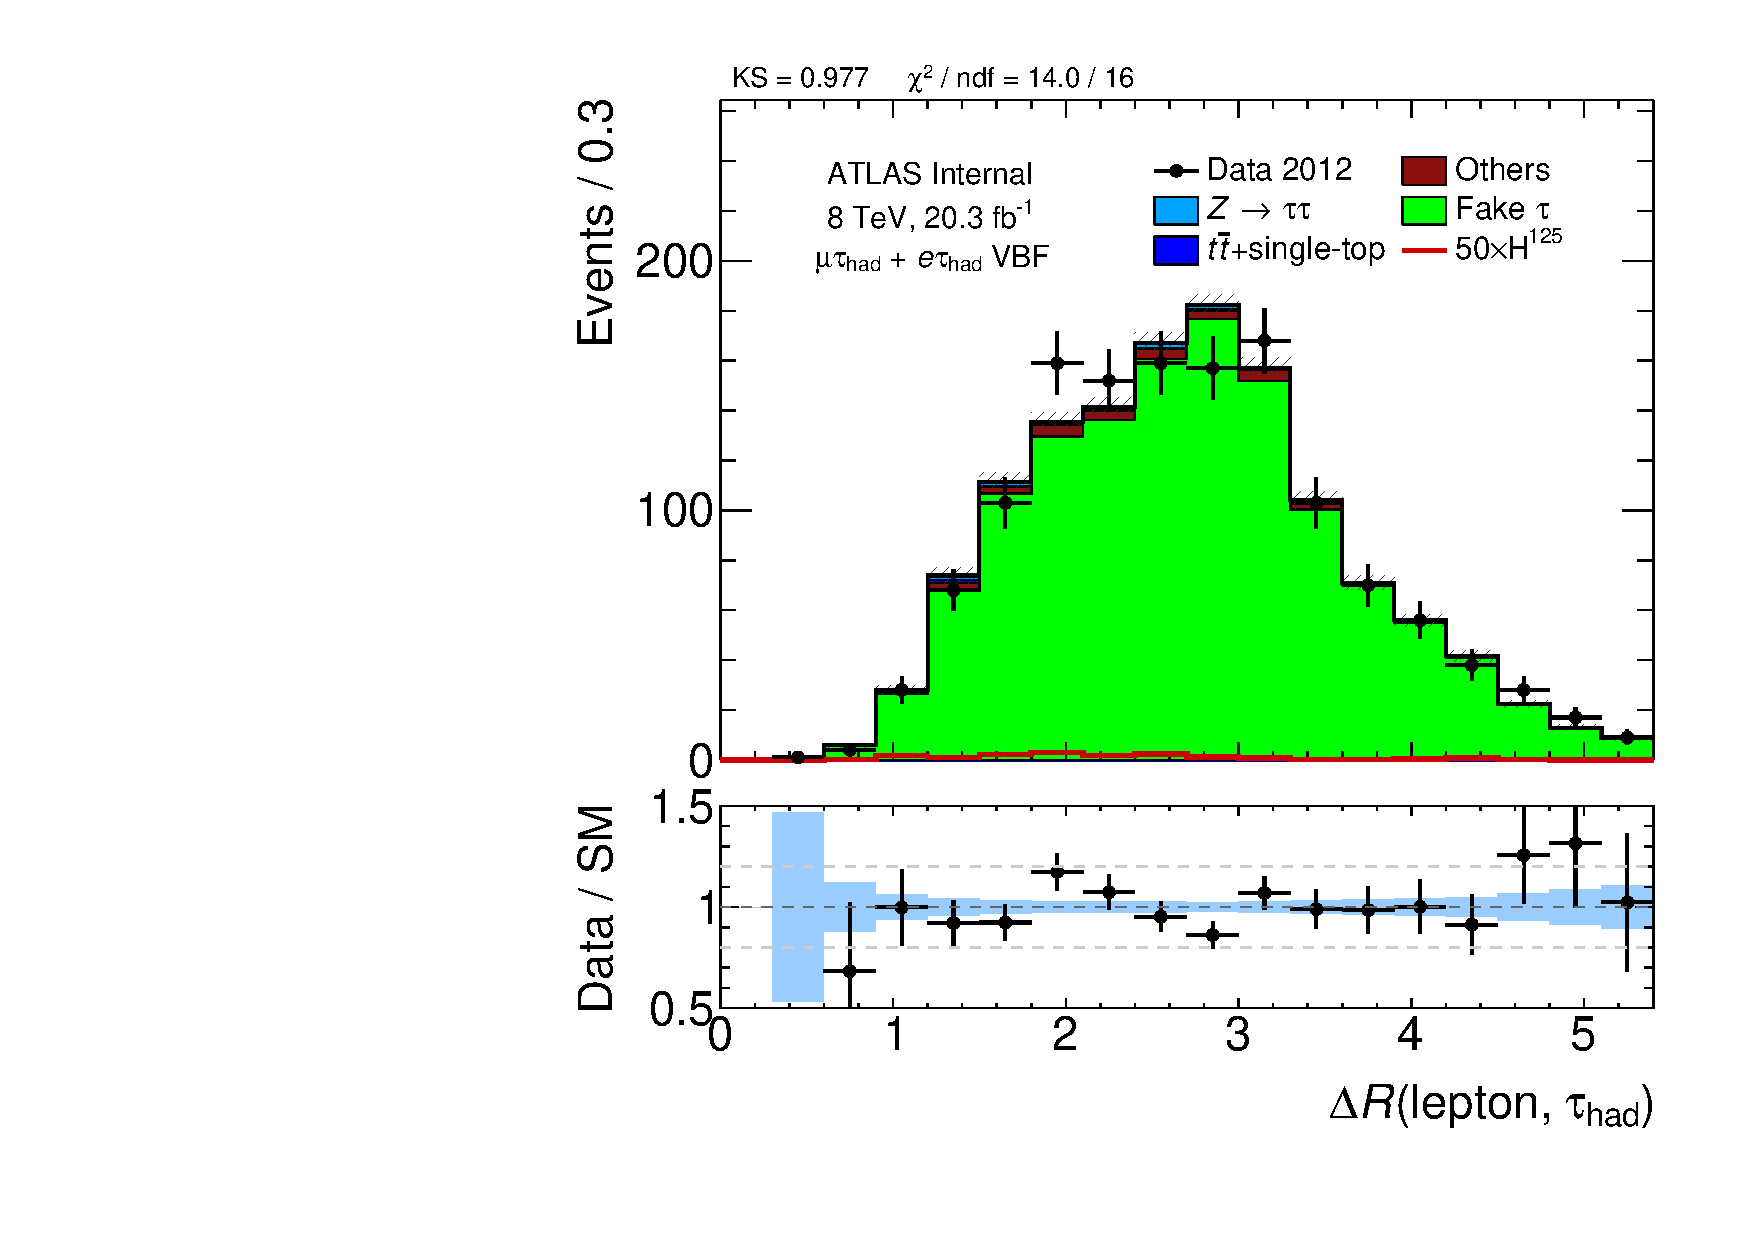
\includegraphics[width=0.32\textwidth]{figures/analysis/vbf-SSXCR/taulep-dR} \\
  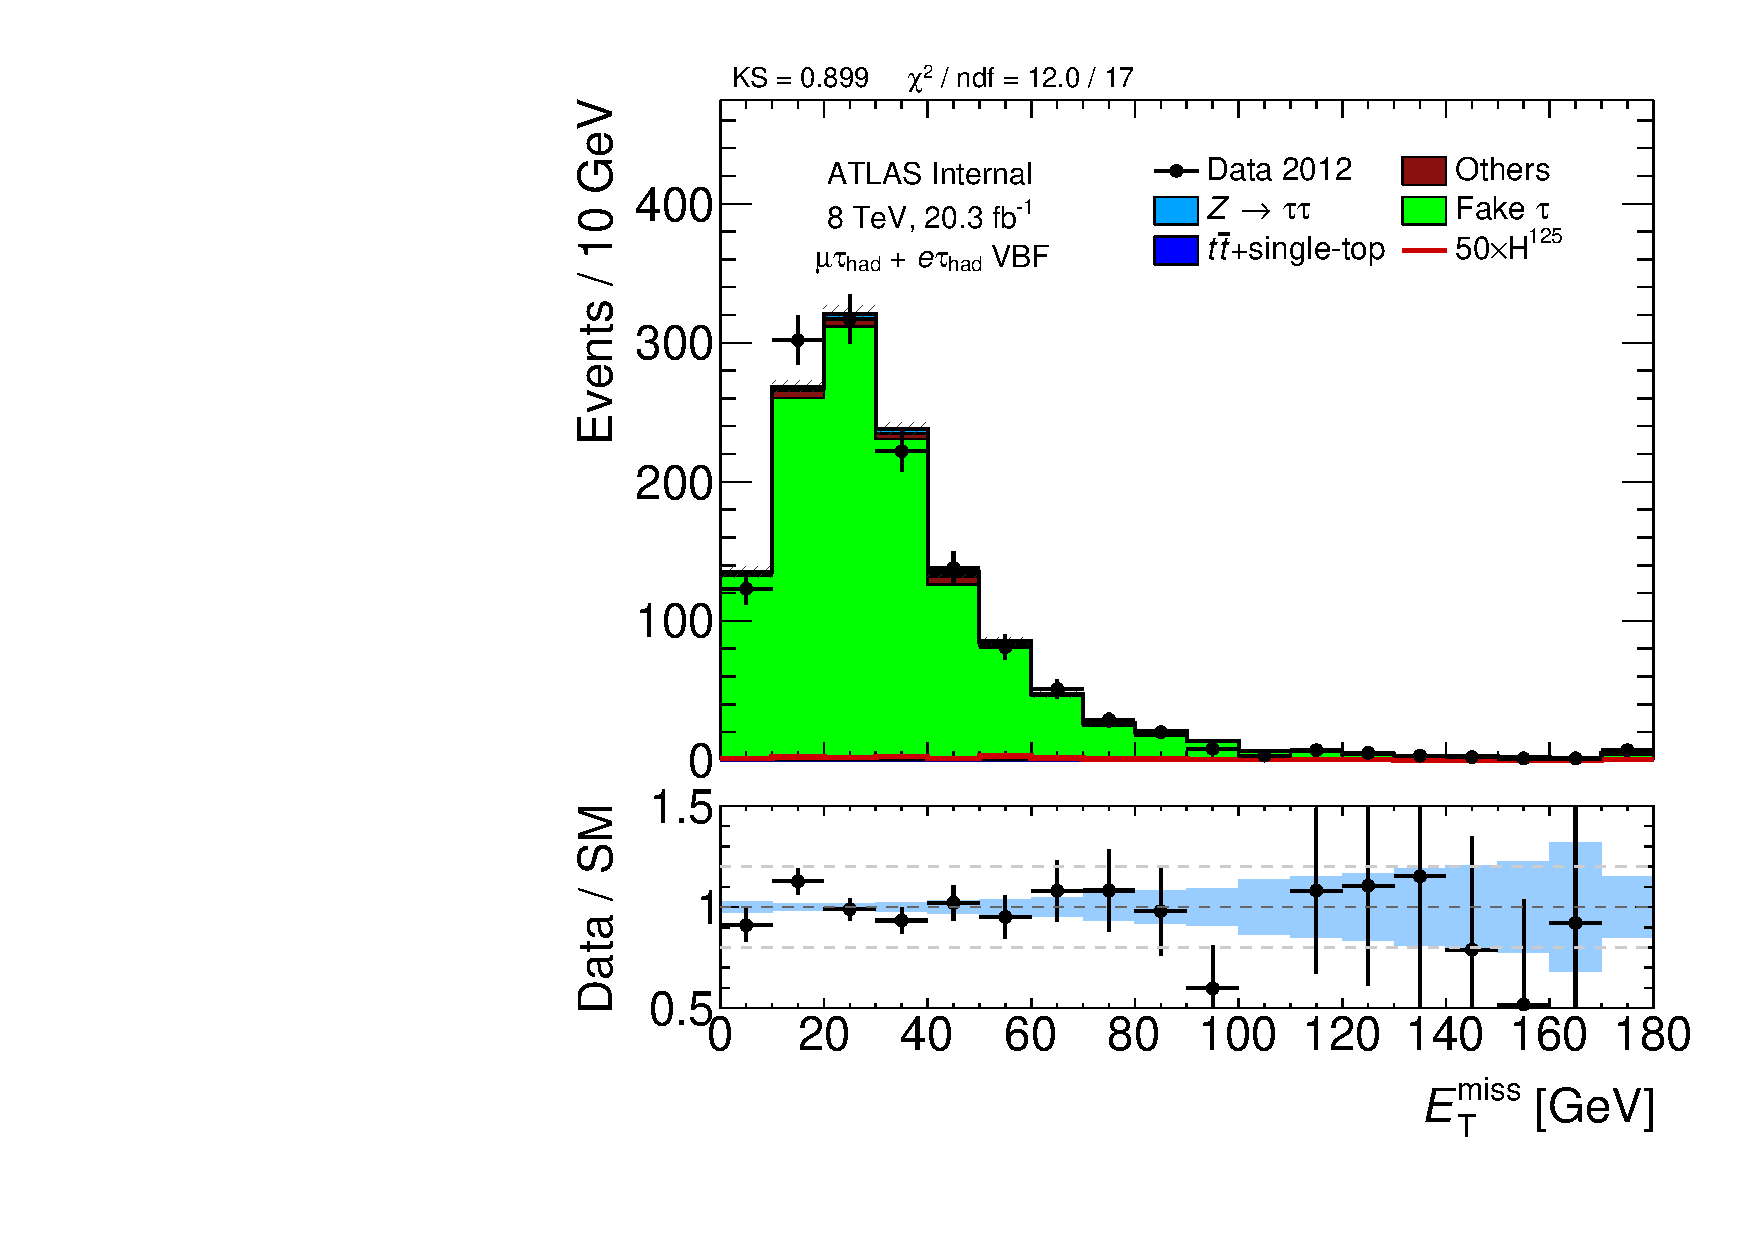
\includegraphics[width=0.32\textwidth]{figures/analysis/vbf-SSXCR/met-pt-hi}
  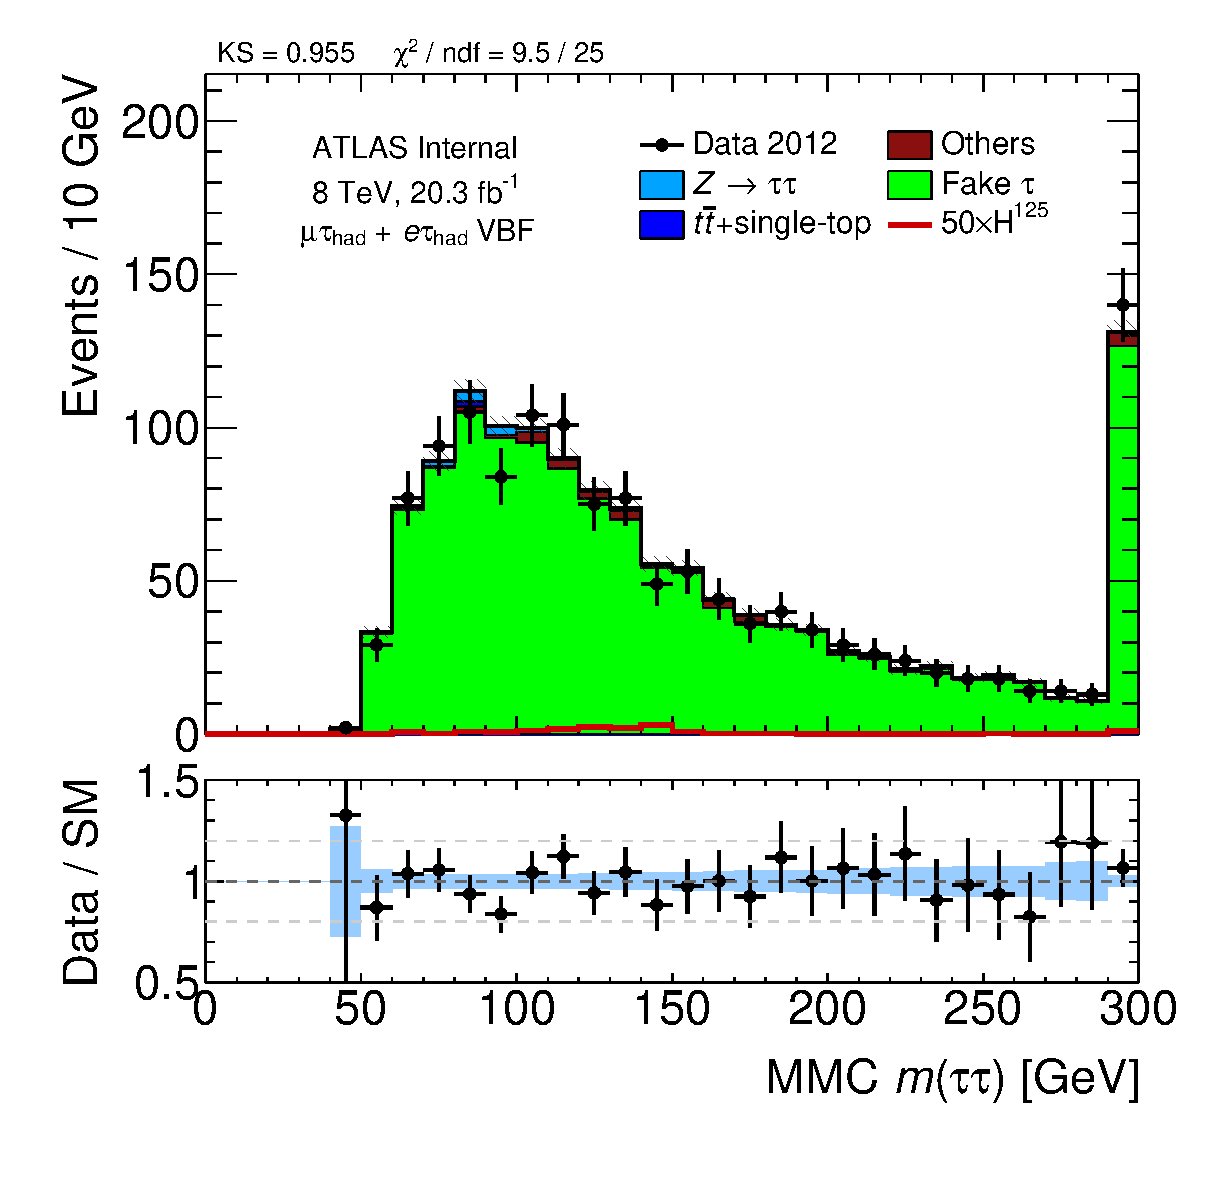
\includegraphics[width=0.32\textwidth]{figures/analysis/vbf-SSXCR/mMMC}
  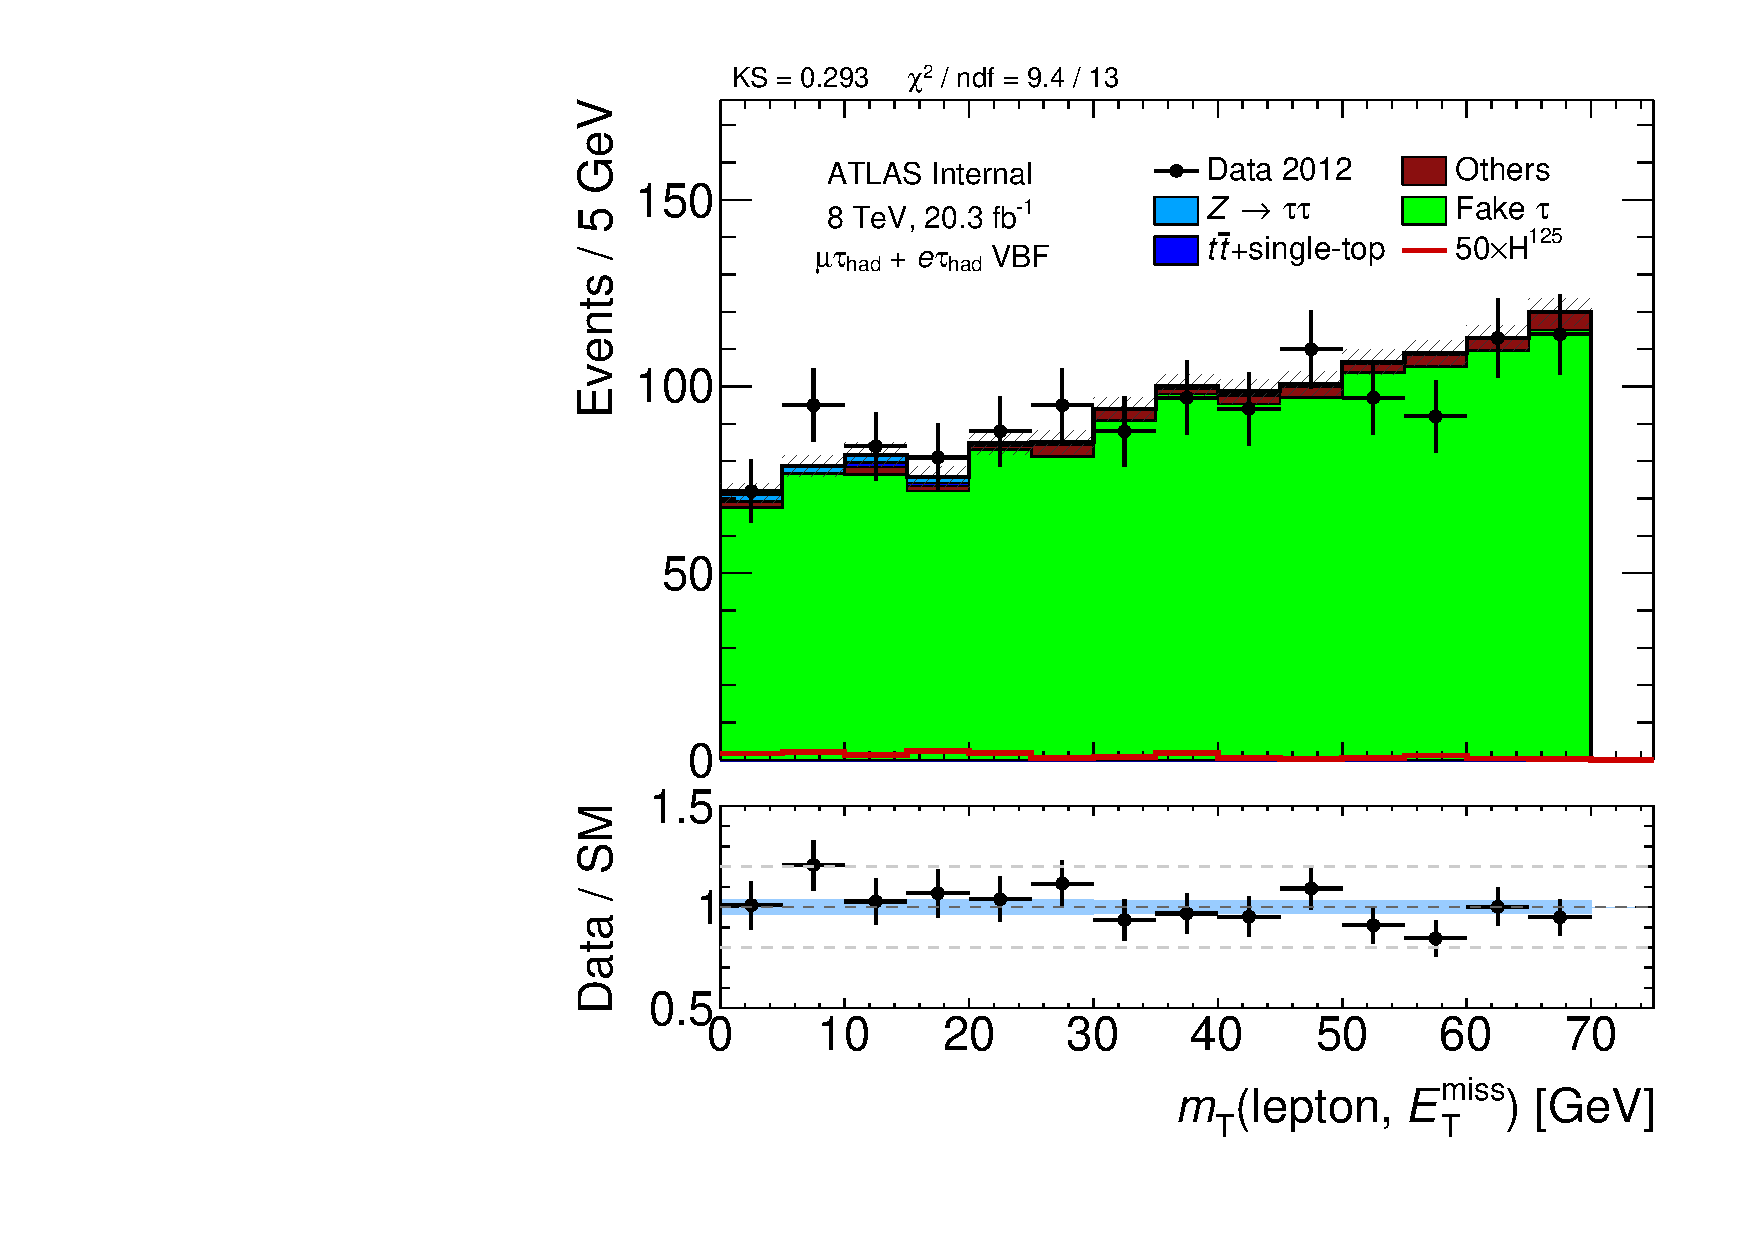
\includegraphics[width=0.32\textwidth]{figures/analysis/vbf-SSXCR/mT} \\
  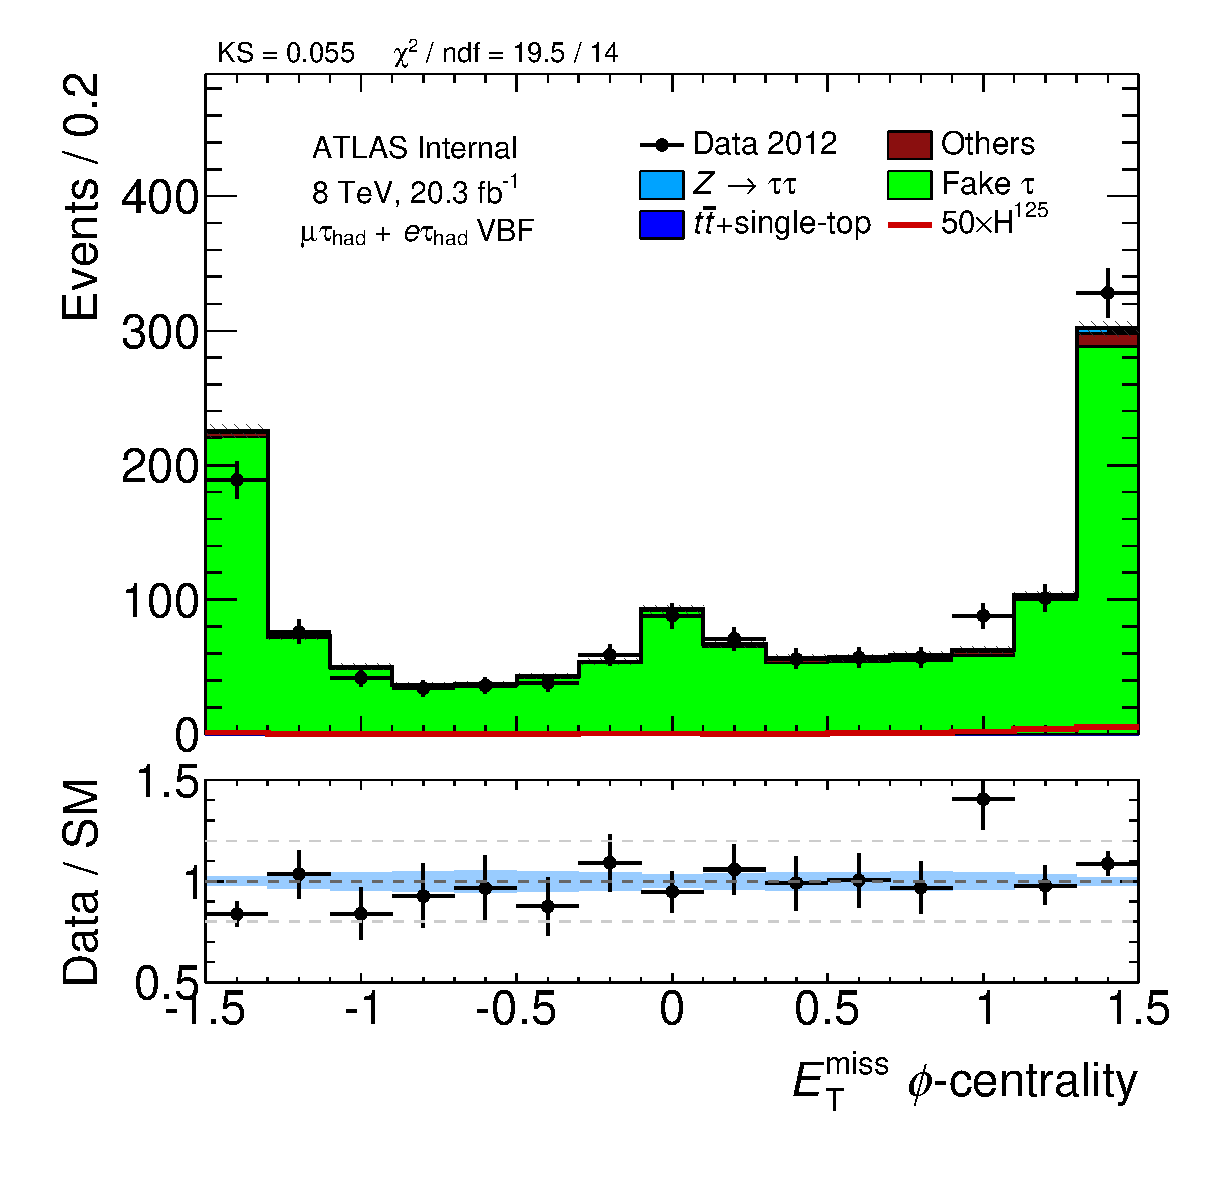
\includegraphics[width=0.32\textwidth]{figures/analysis/vbf-SSXCR/met-phi-centrality}
  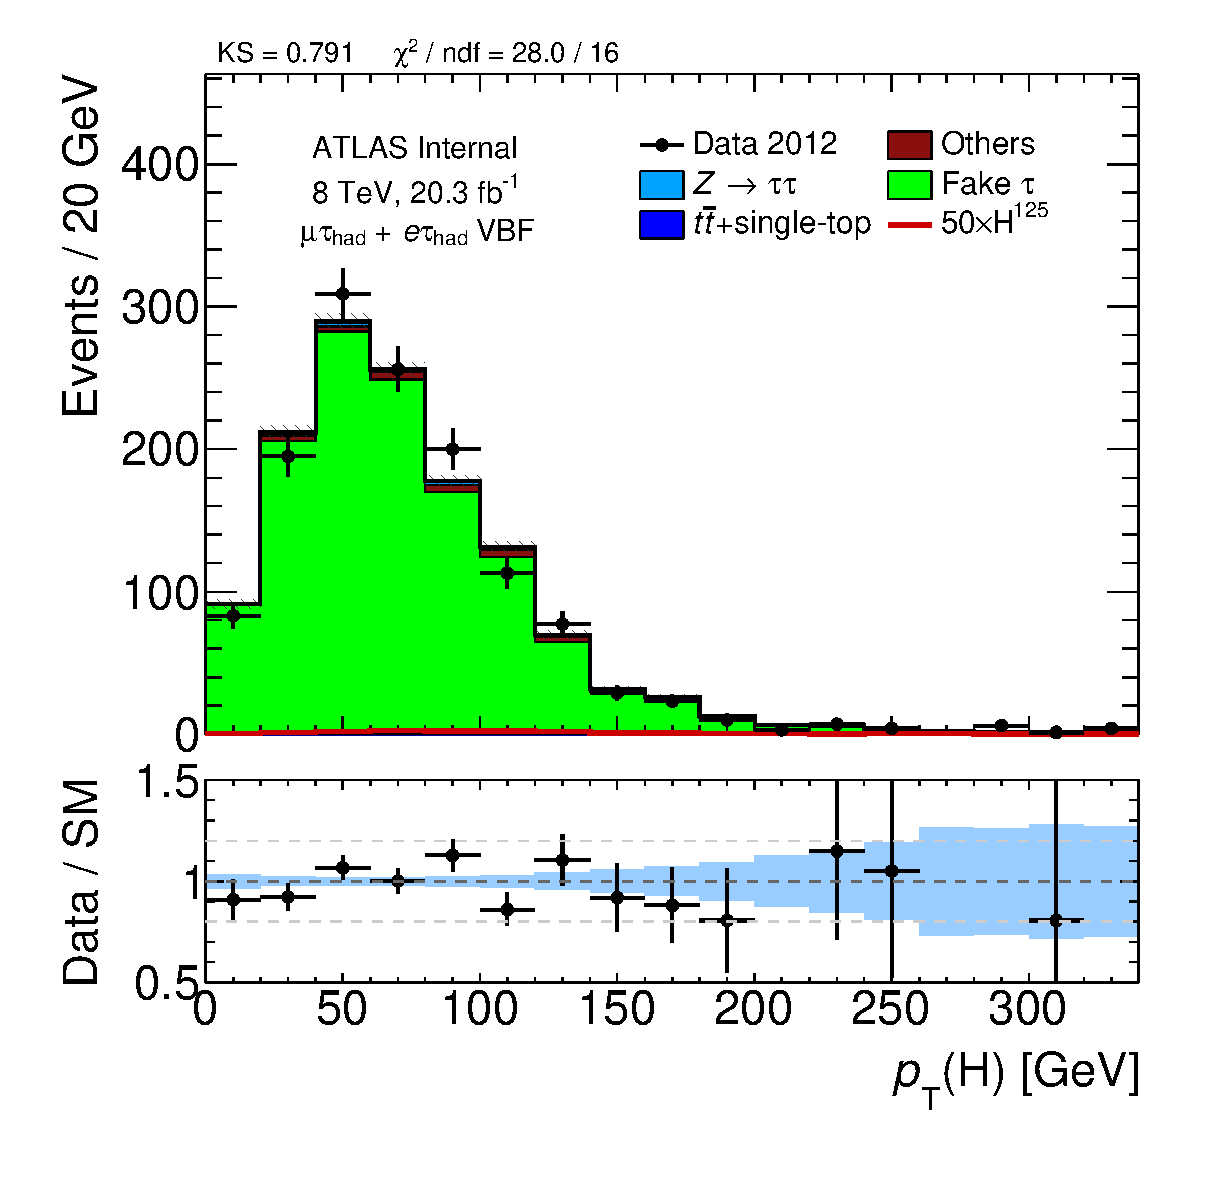
\includegraphics[width=0.32\textwidth]{figures/analysis/vbf-SSXCR/H-pt-hi}
  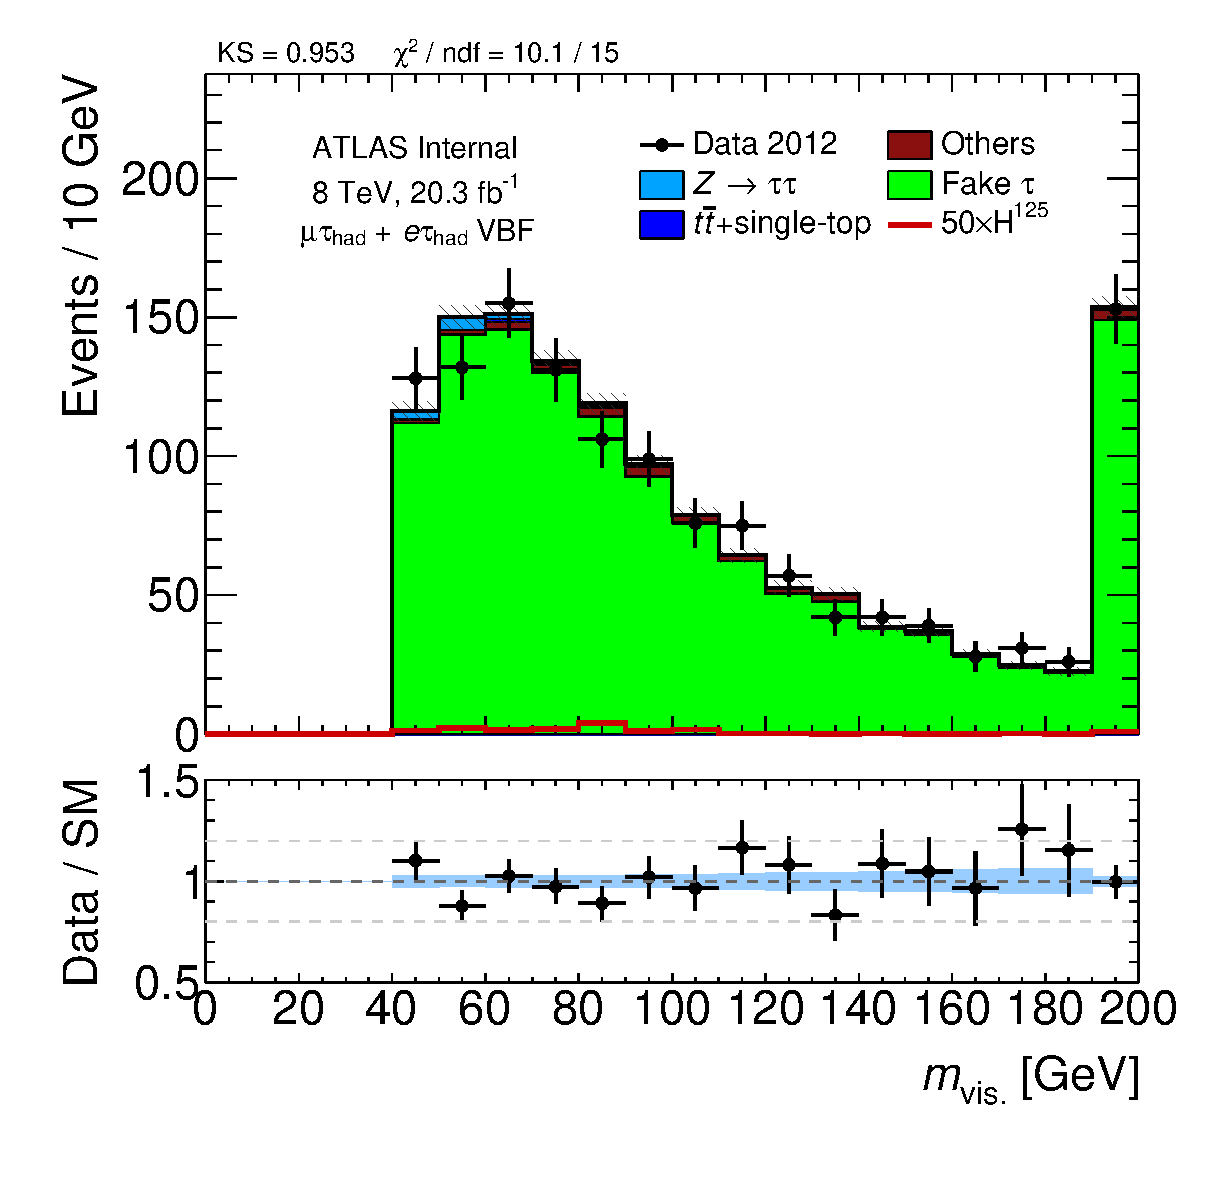
\includegraphics[width=0.32\textwidth]{figures/analysis/vbf-SSXCR/mvis} \\
  \caption{Comparison of data and $\fakes$ prediction in the same sign CR for various event kinematics. Only statistical uncertainties are shown.}
  \label{fig:backgrounds-SSXCR-taus}
\end{figure}

\begin{figure}[tp]
  \centering
  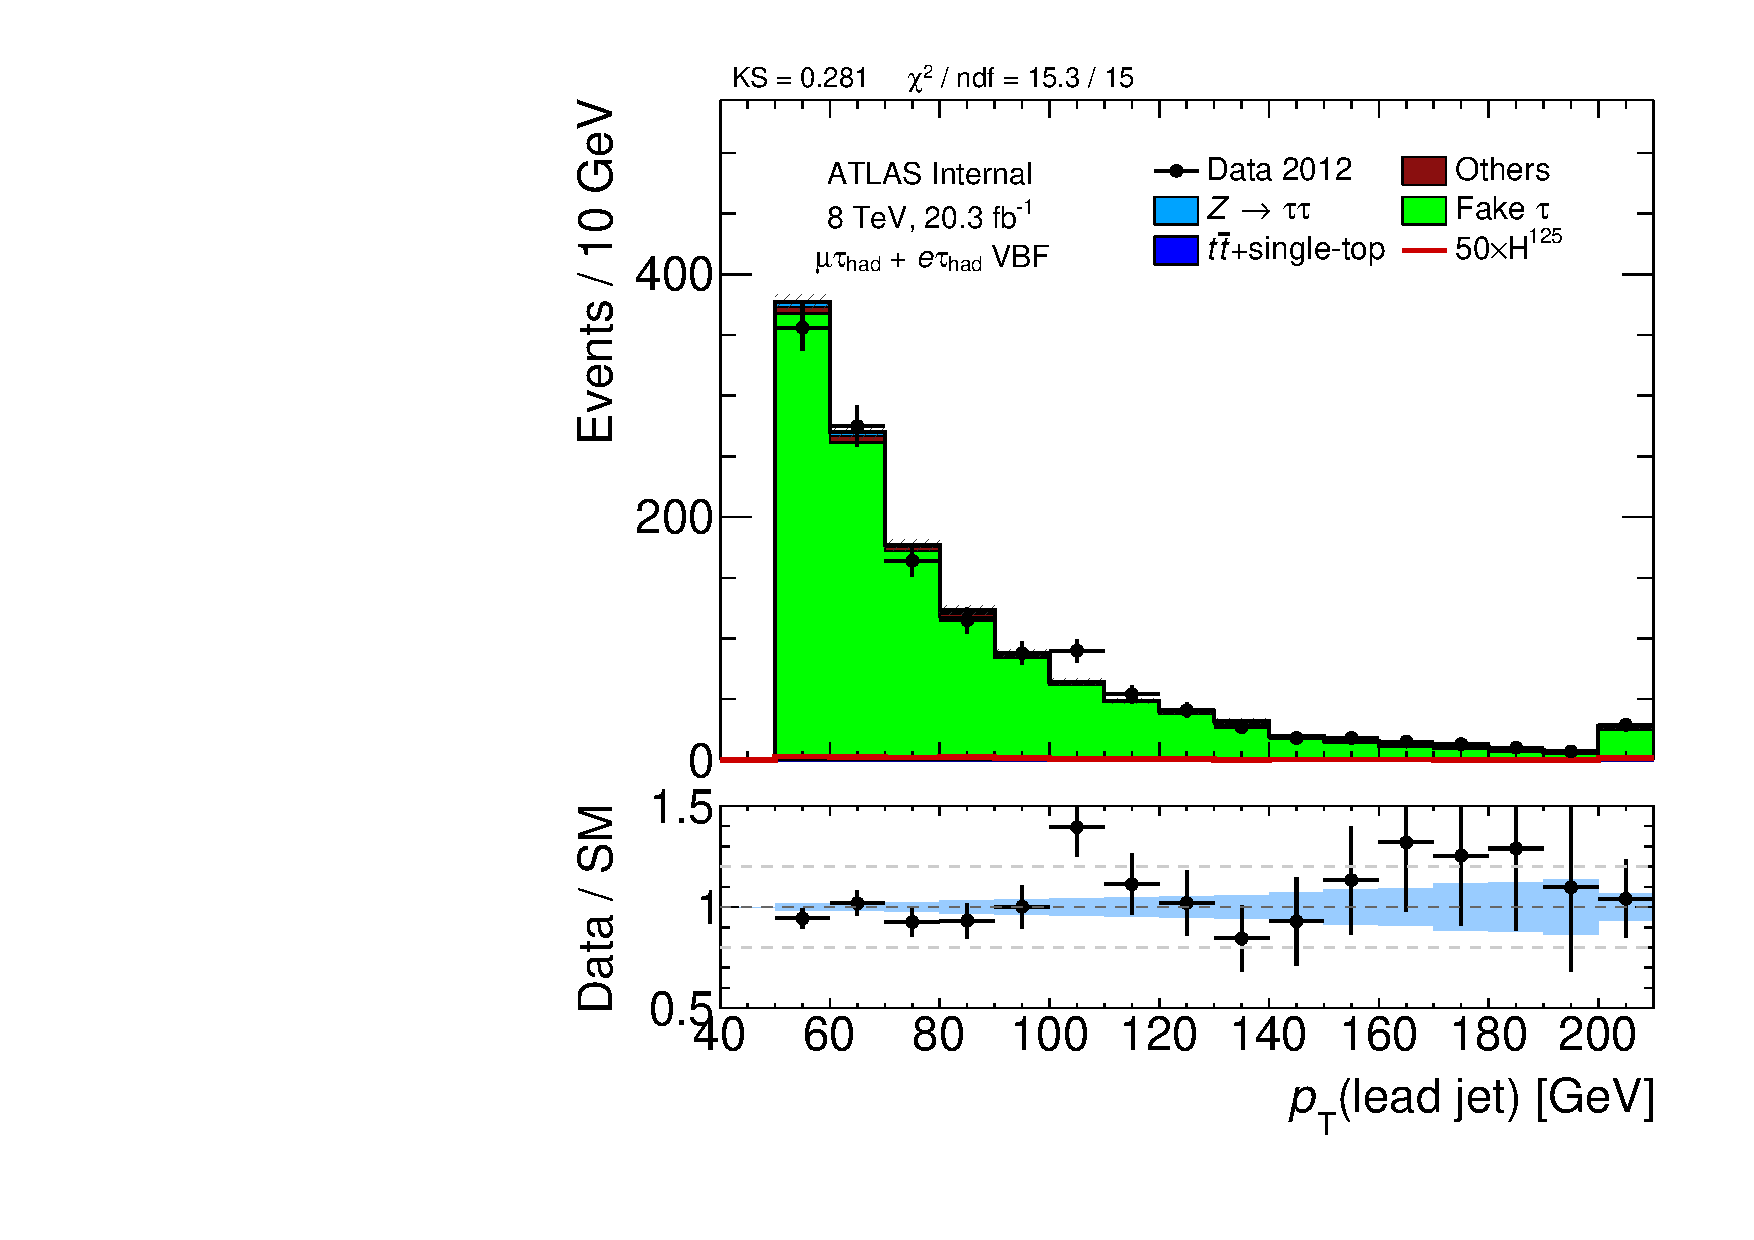
\includegraphics[width=0.32\textwidth]{figures/analysis/vbf-SSXCR/jet-1-pt}
  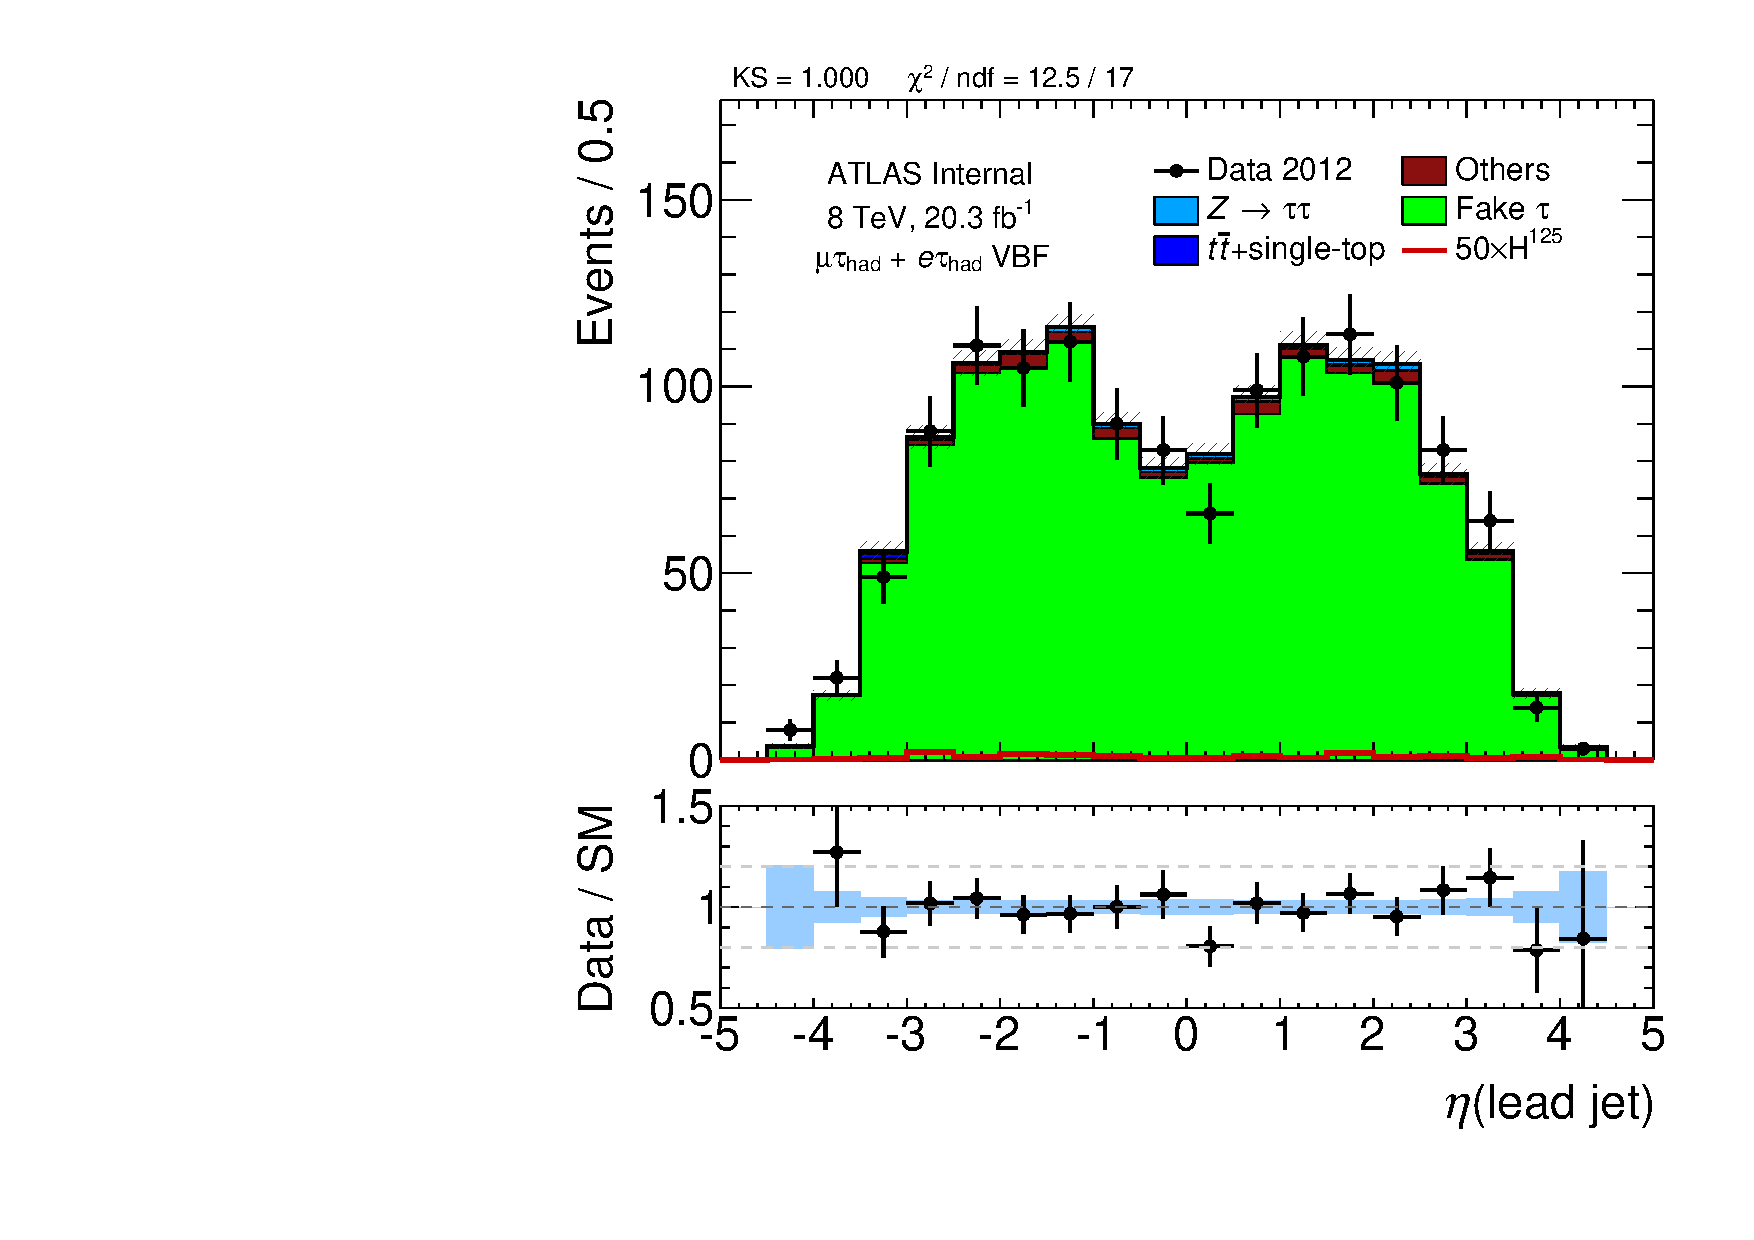
\includegraphics[width=0.32\textwidth]{figures/analysis/vbf-SSXCR/jet-1-eta}
  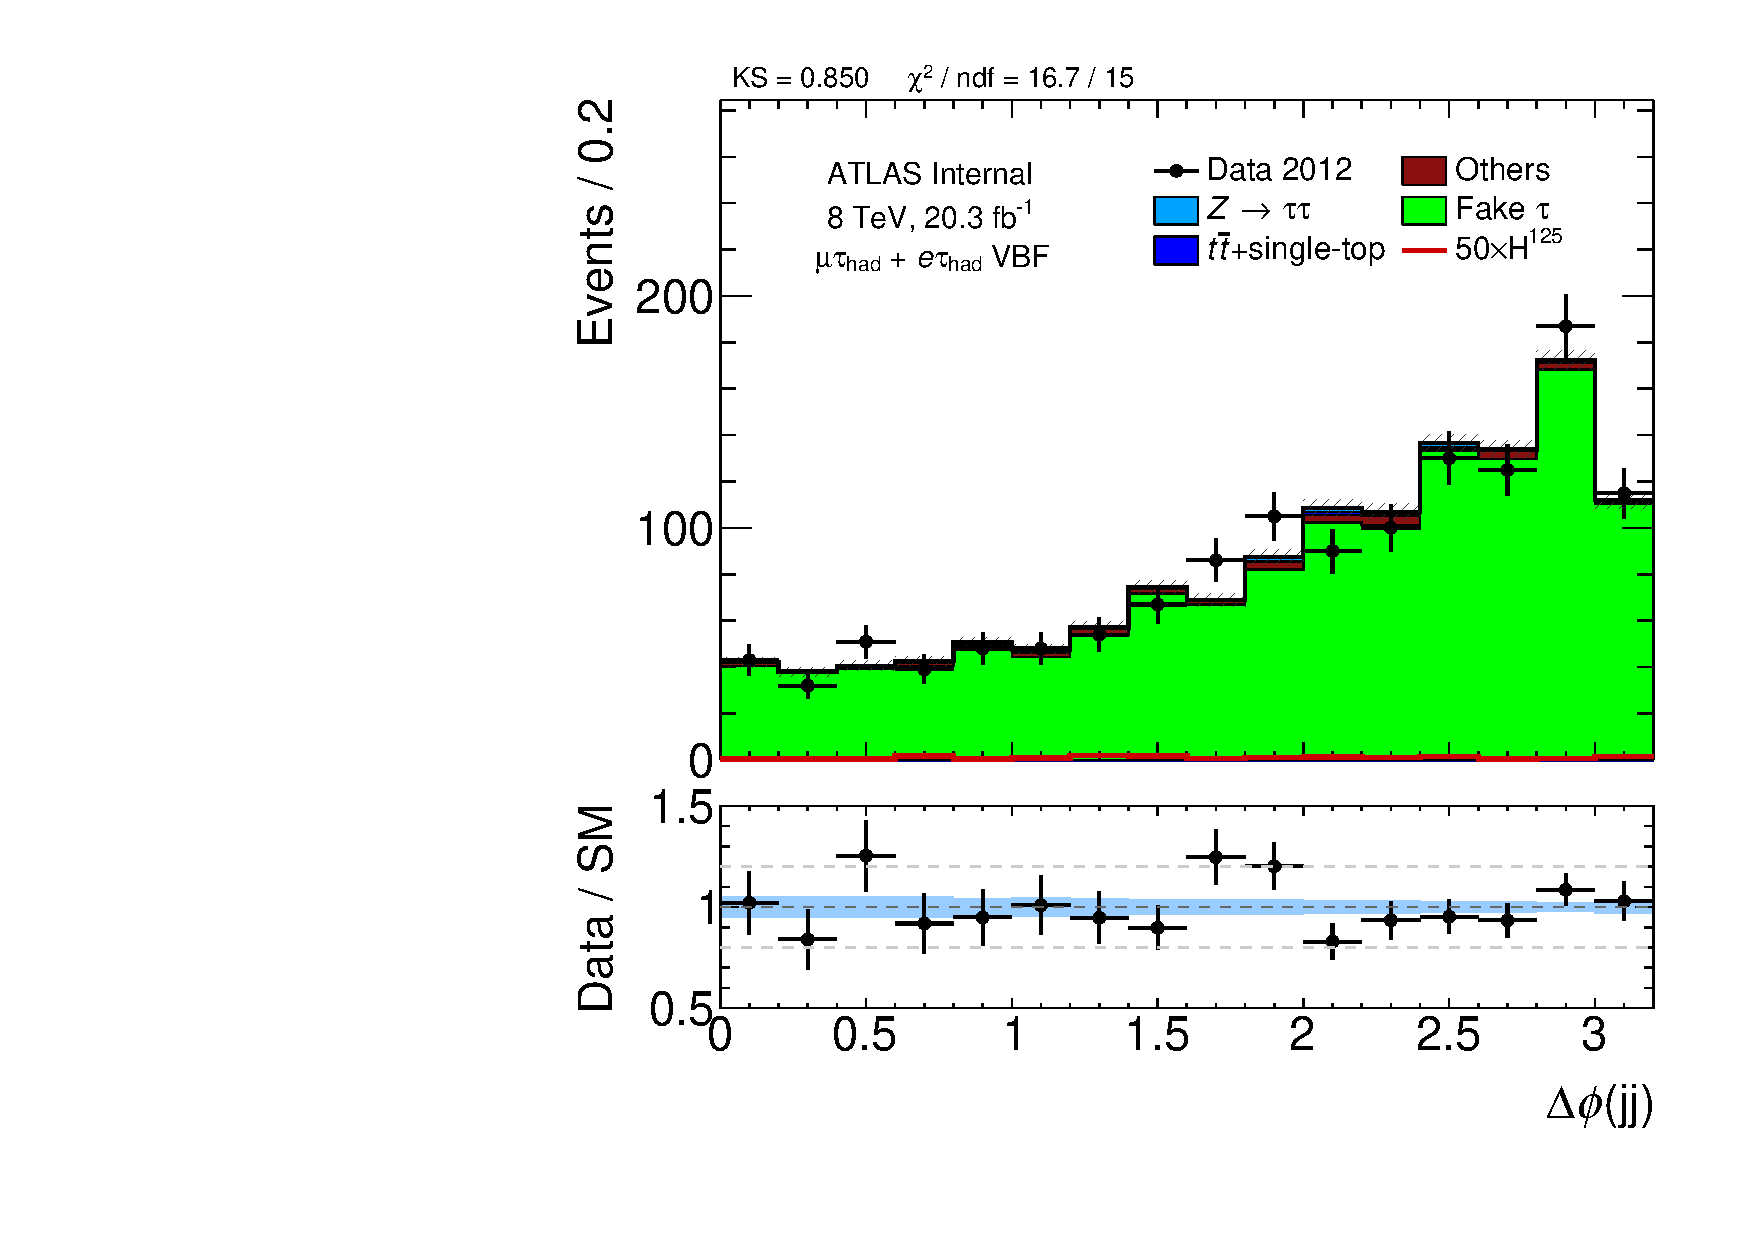
\includegraphics[width=0.32\textwidth]{figures/analysis/vbf-SSXCR/jets-dphi} \\
  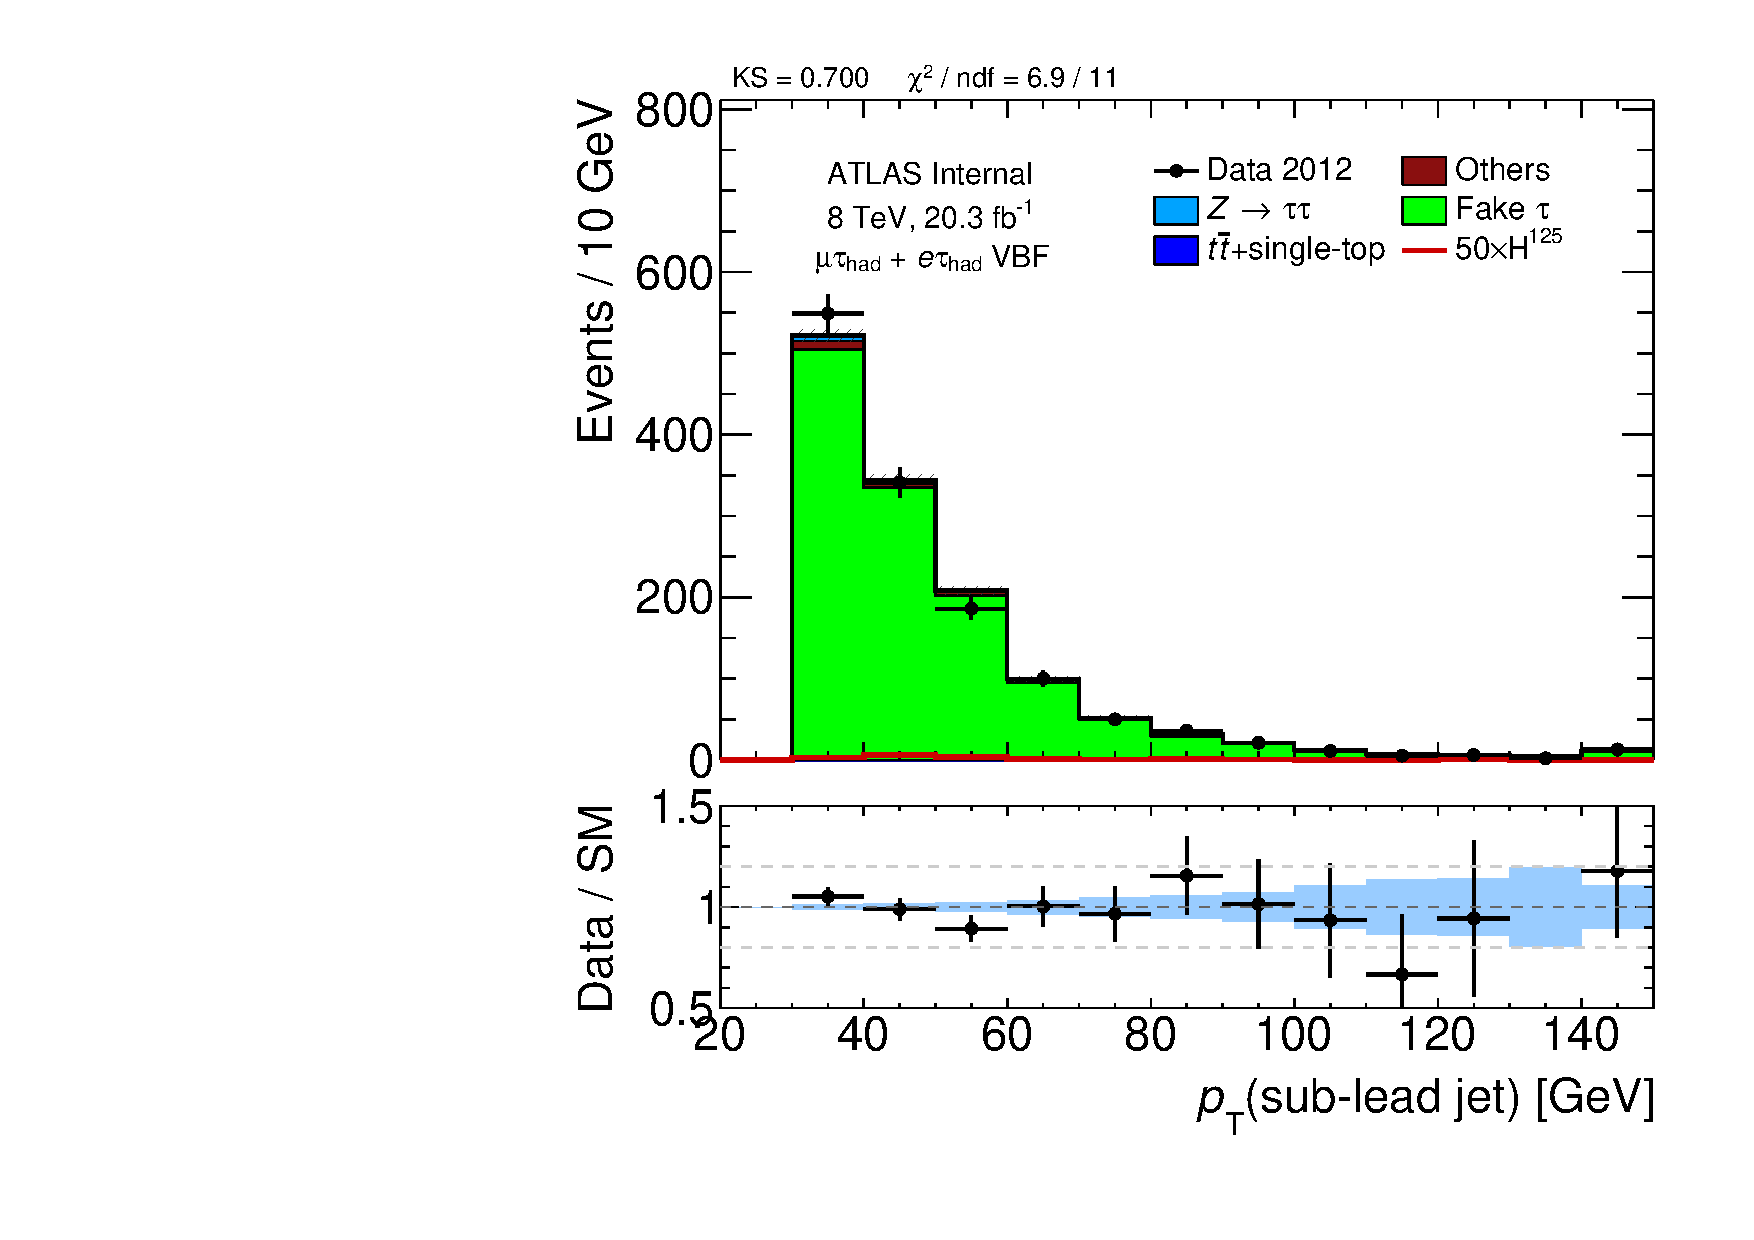
\includegraphics[width=0.32\textwidth]{figures/analysis/vbf-SSXCR/jet-2-pt}
  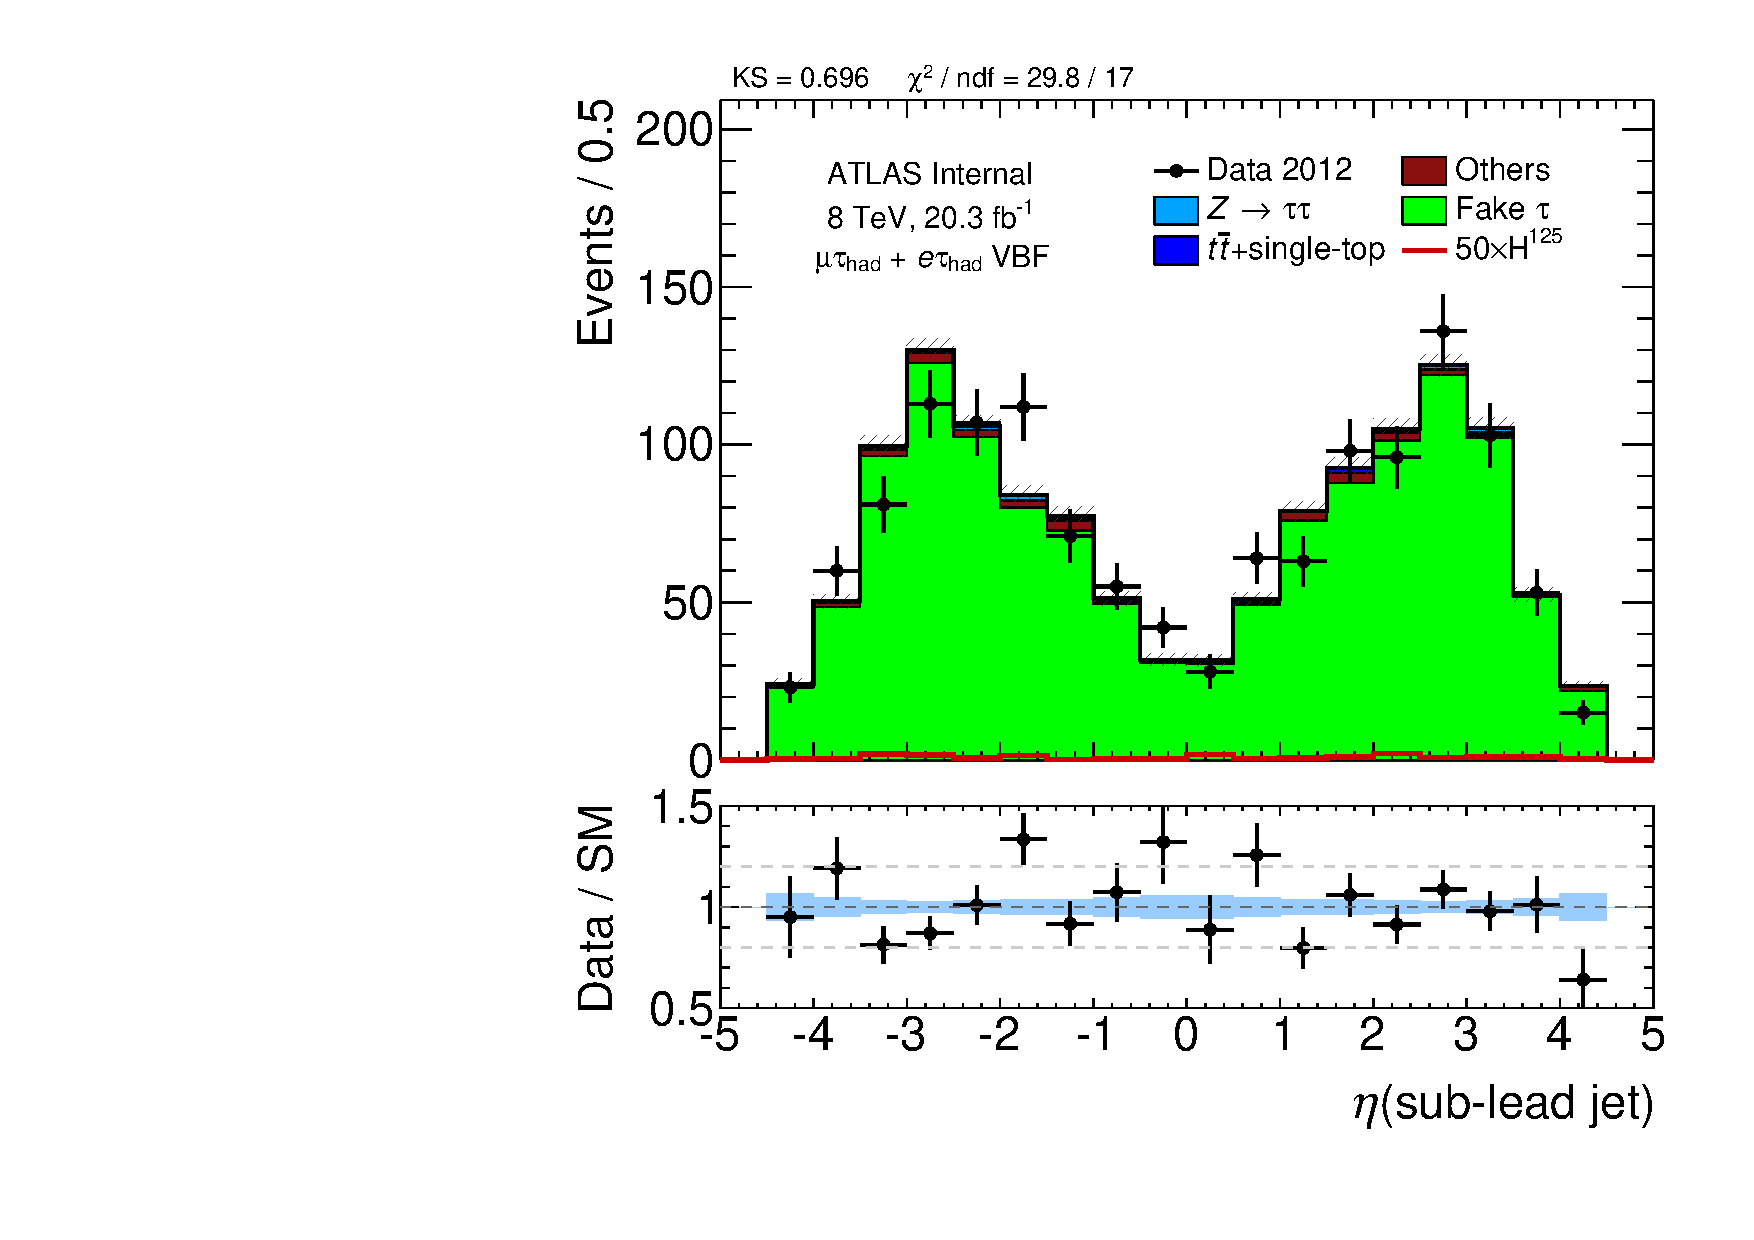
\includegraphics[width=0.32\textwidth]{figures/analysis/vbf-SSXCR/jet-2-eta}
  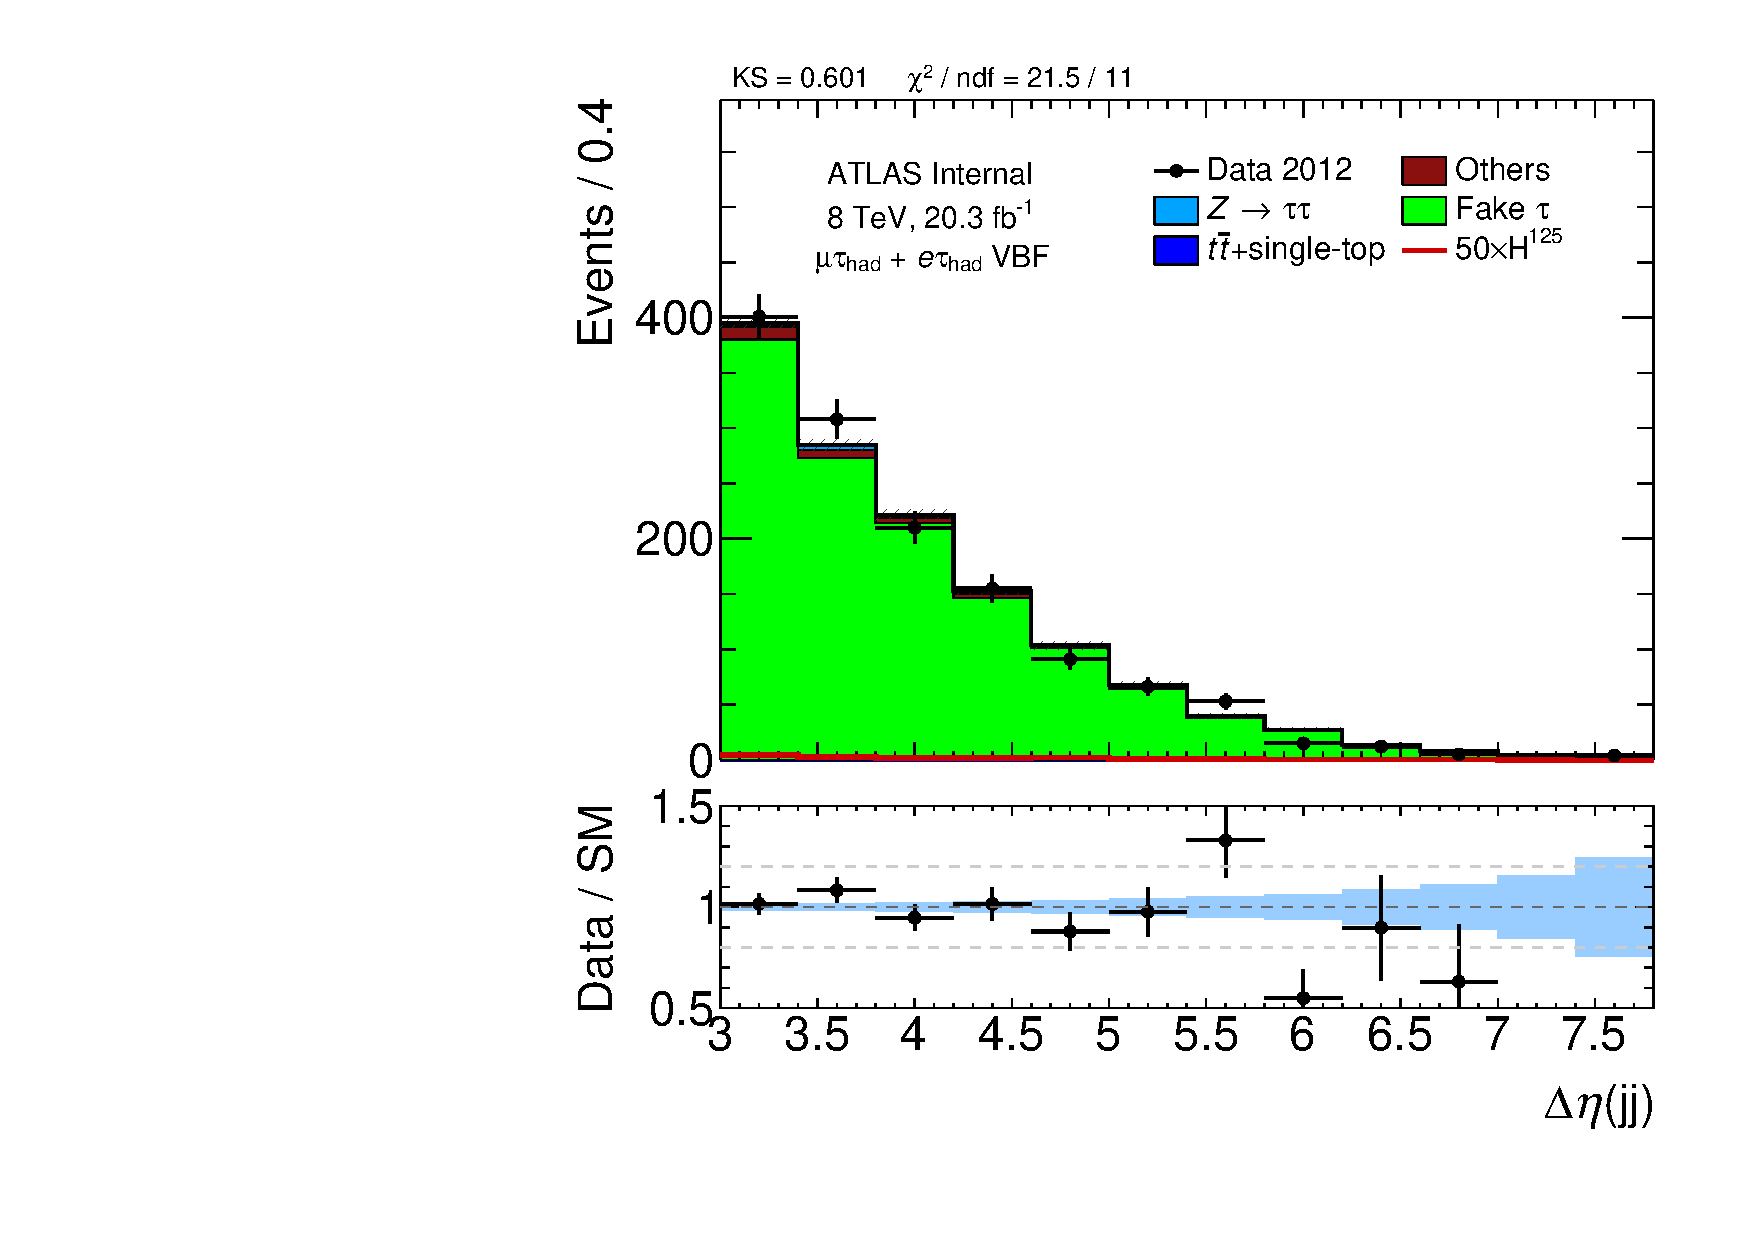
\includegraphics[width=0.32\textwidth]{figures/analysis/vbf-SSXCR/jets-deta} \\
  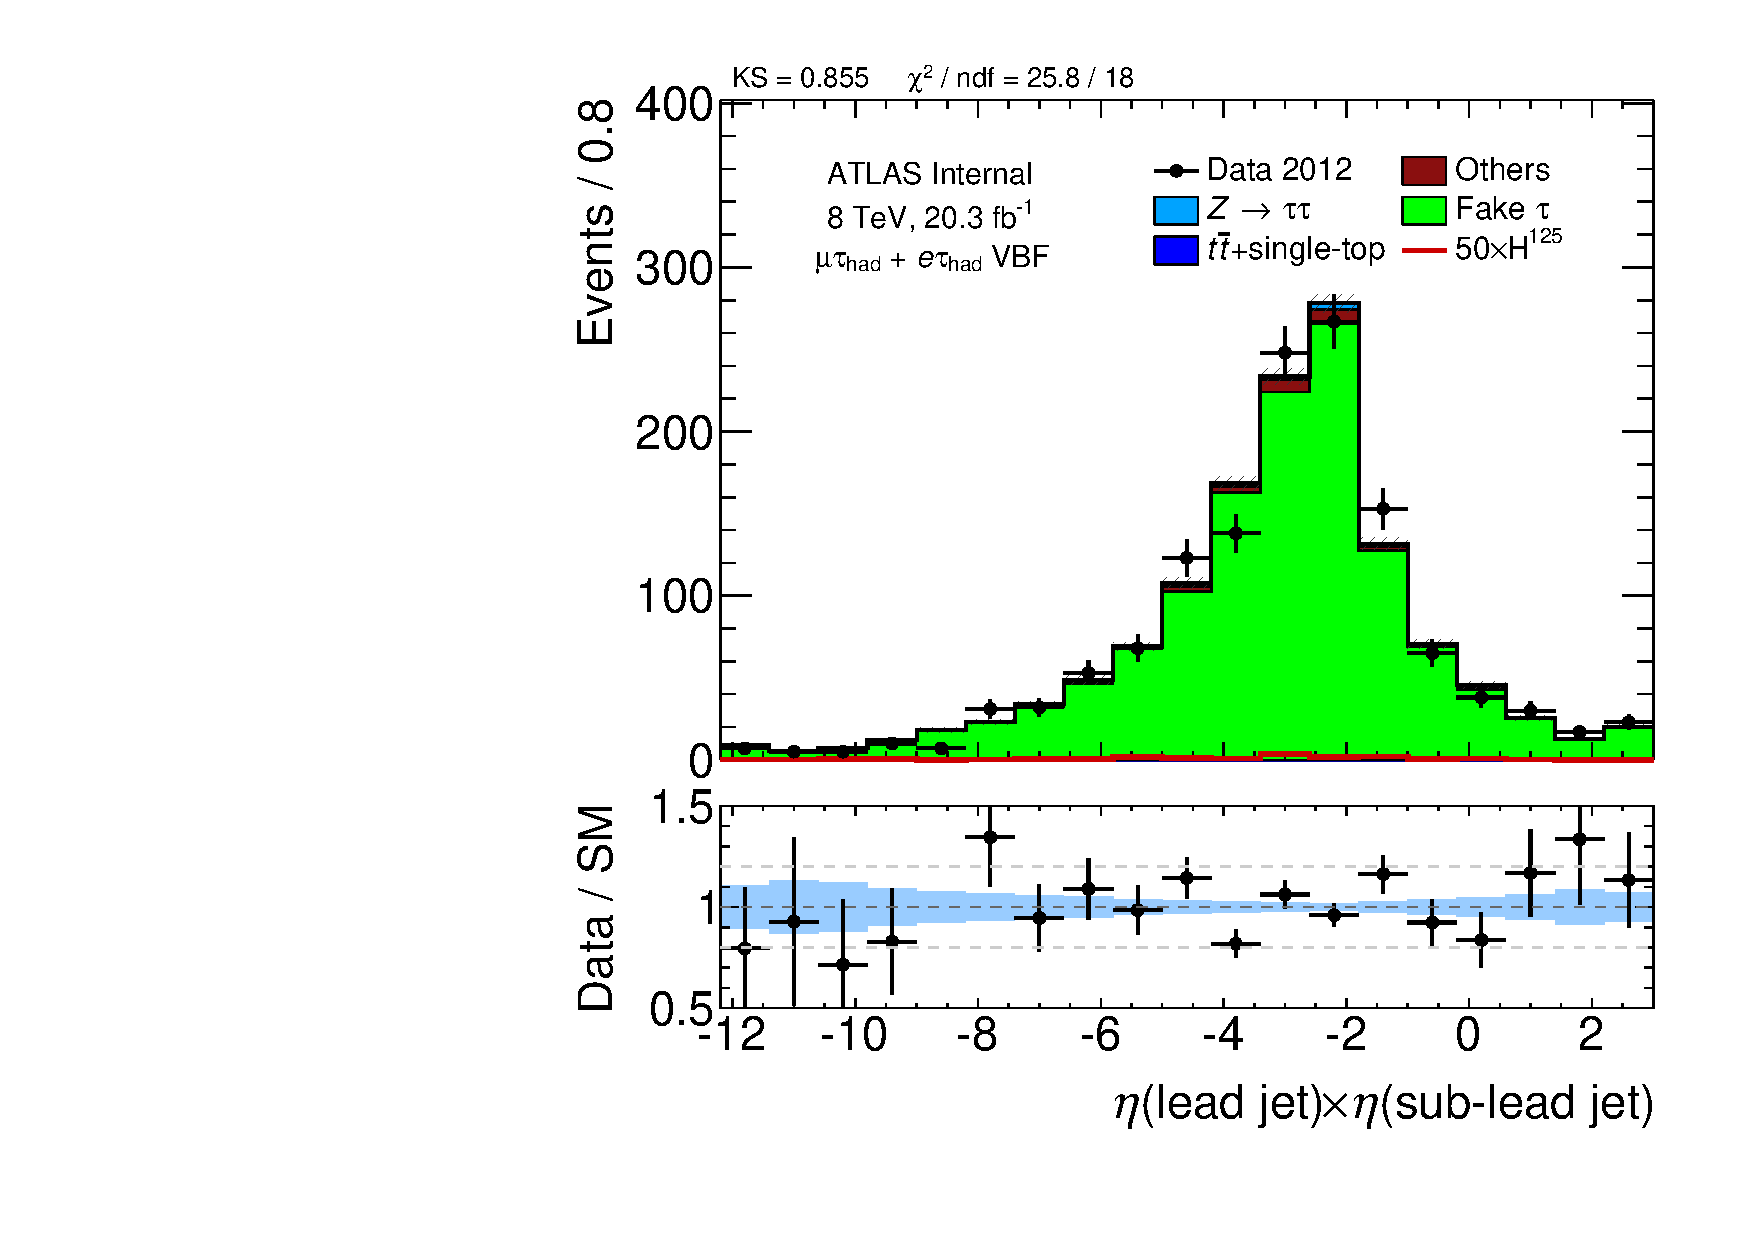
\includegraphics[width=0.32\textwidth]{figures/analysis/vbf-SSXCR/jets-etaprod} 
  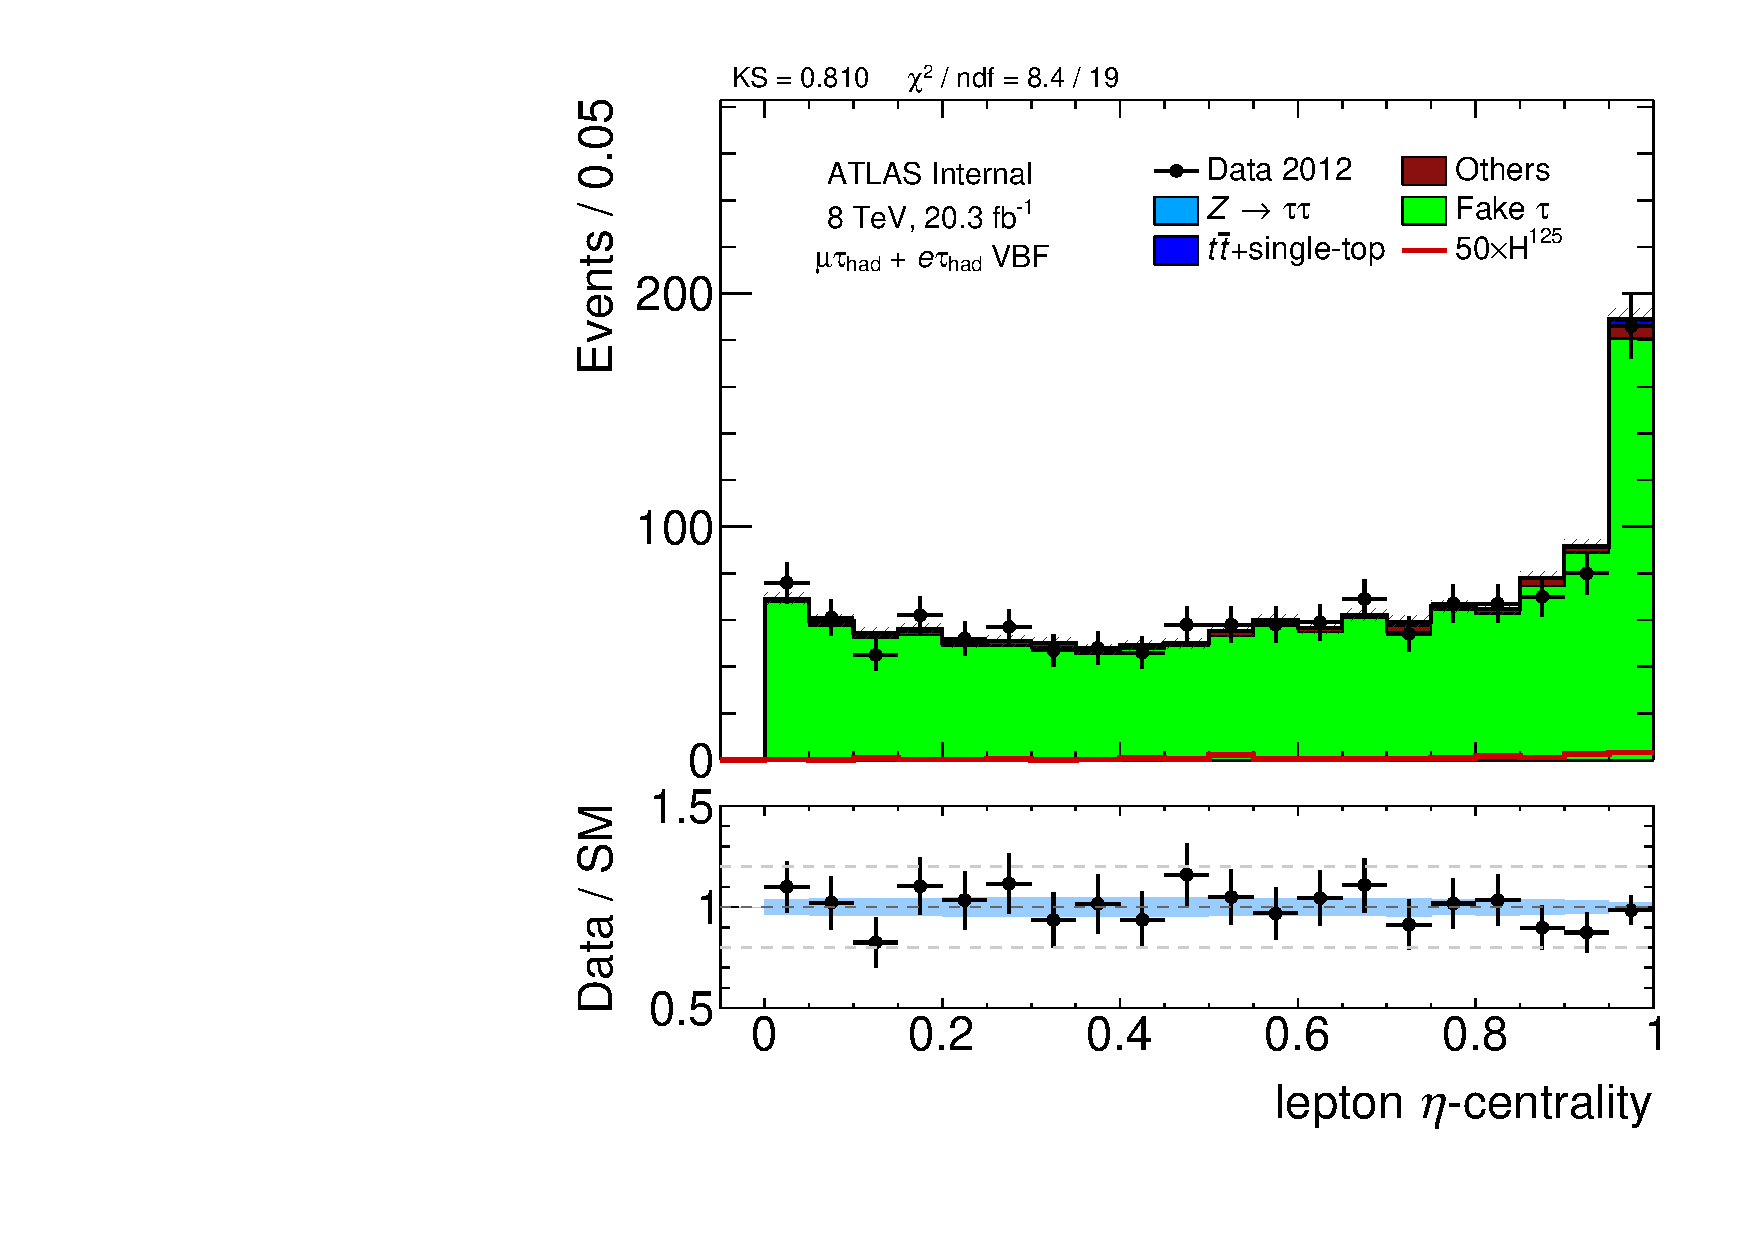
\includegraphics[width=0.32\textwidth]{figures/analysis/vbf-SSXCR/lep-eta-centrality}
  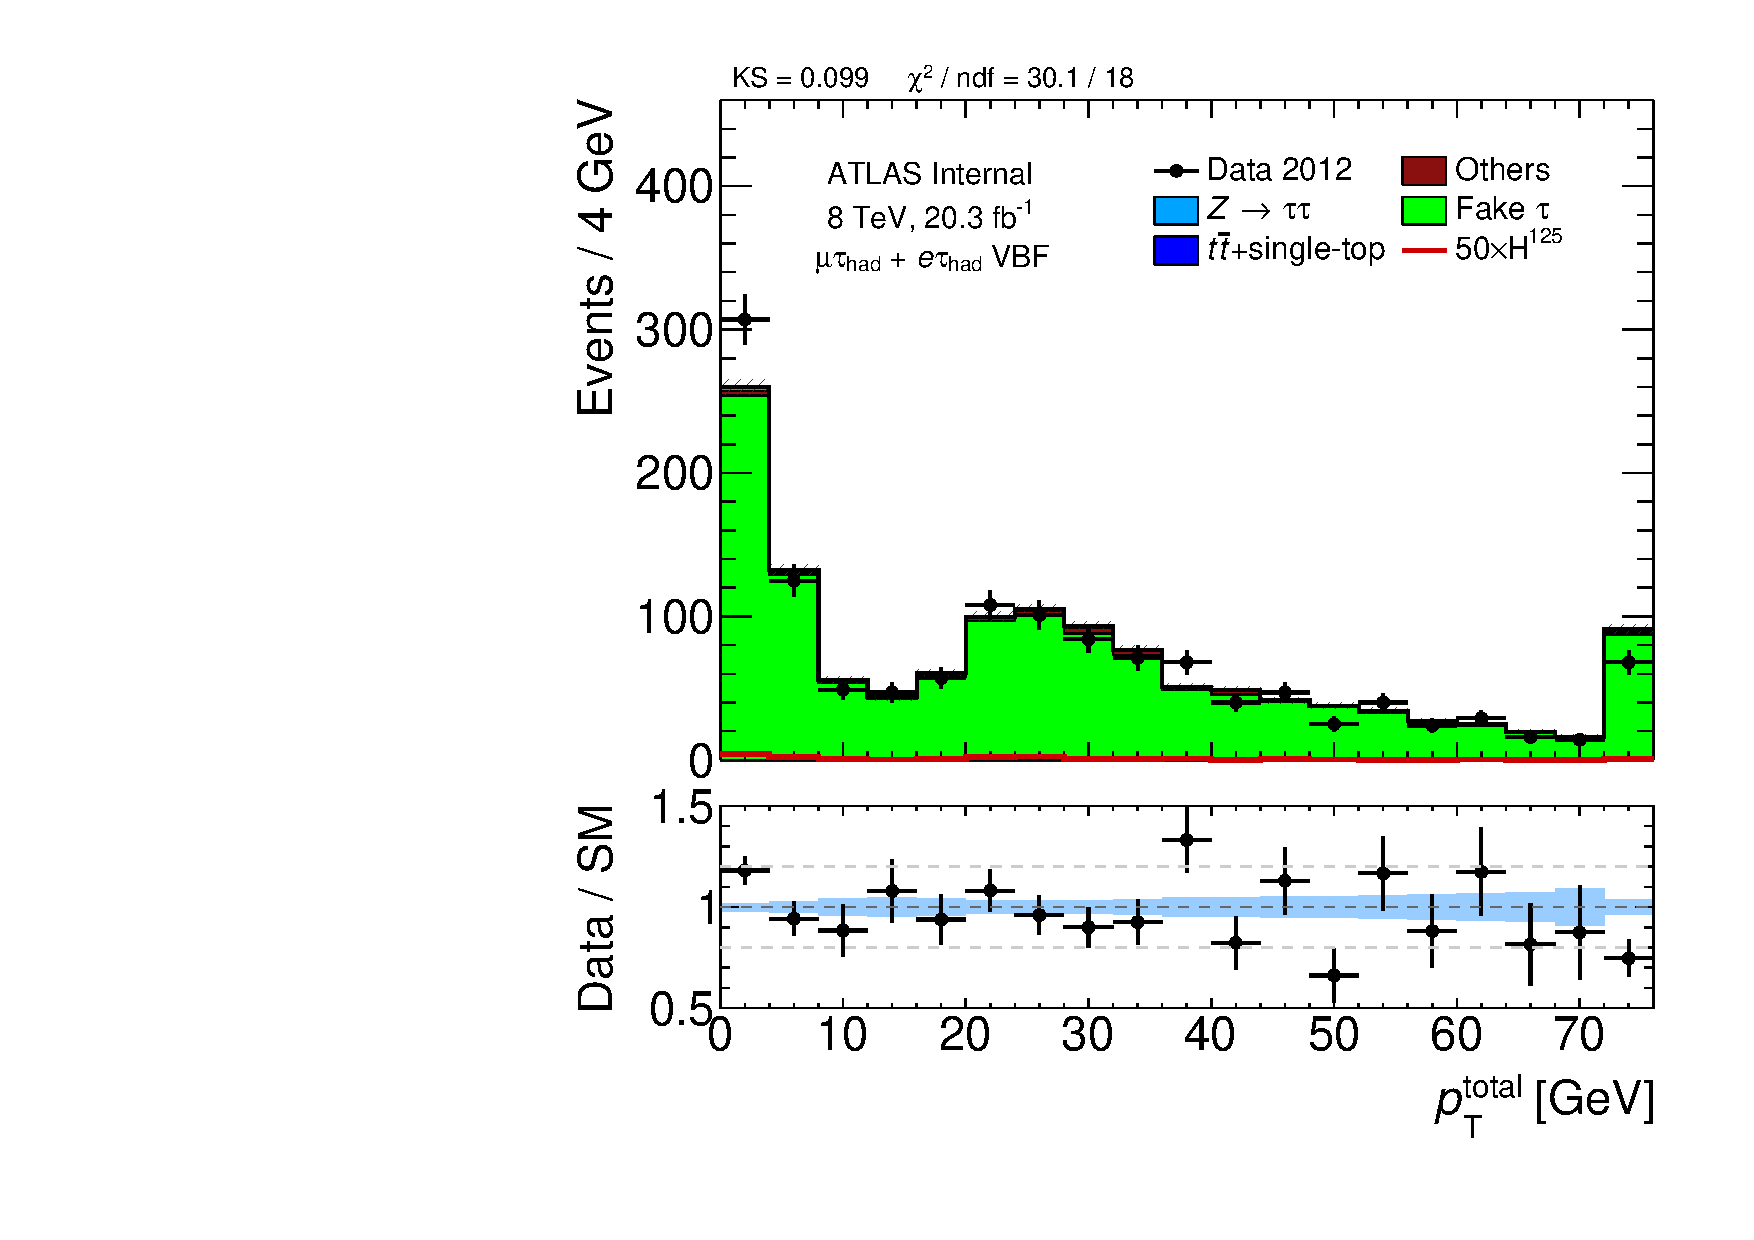
\includegraphics[width=0.32\textwidth]{figures/analysis/vbf-SSXCR/system-pt} \\
  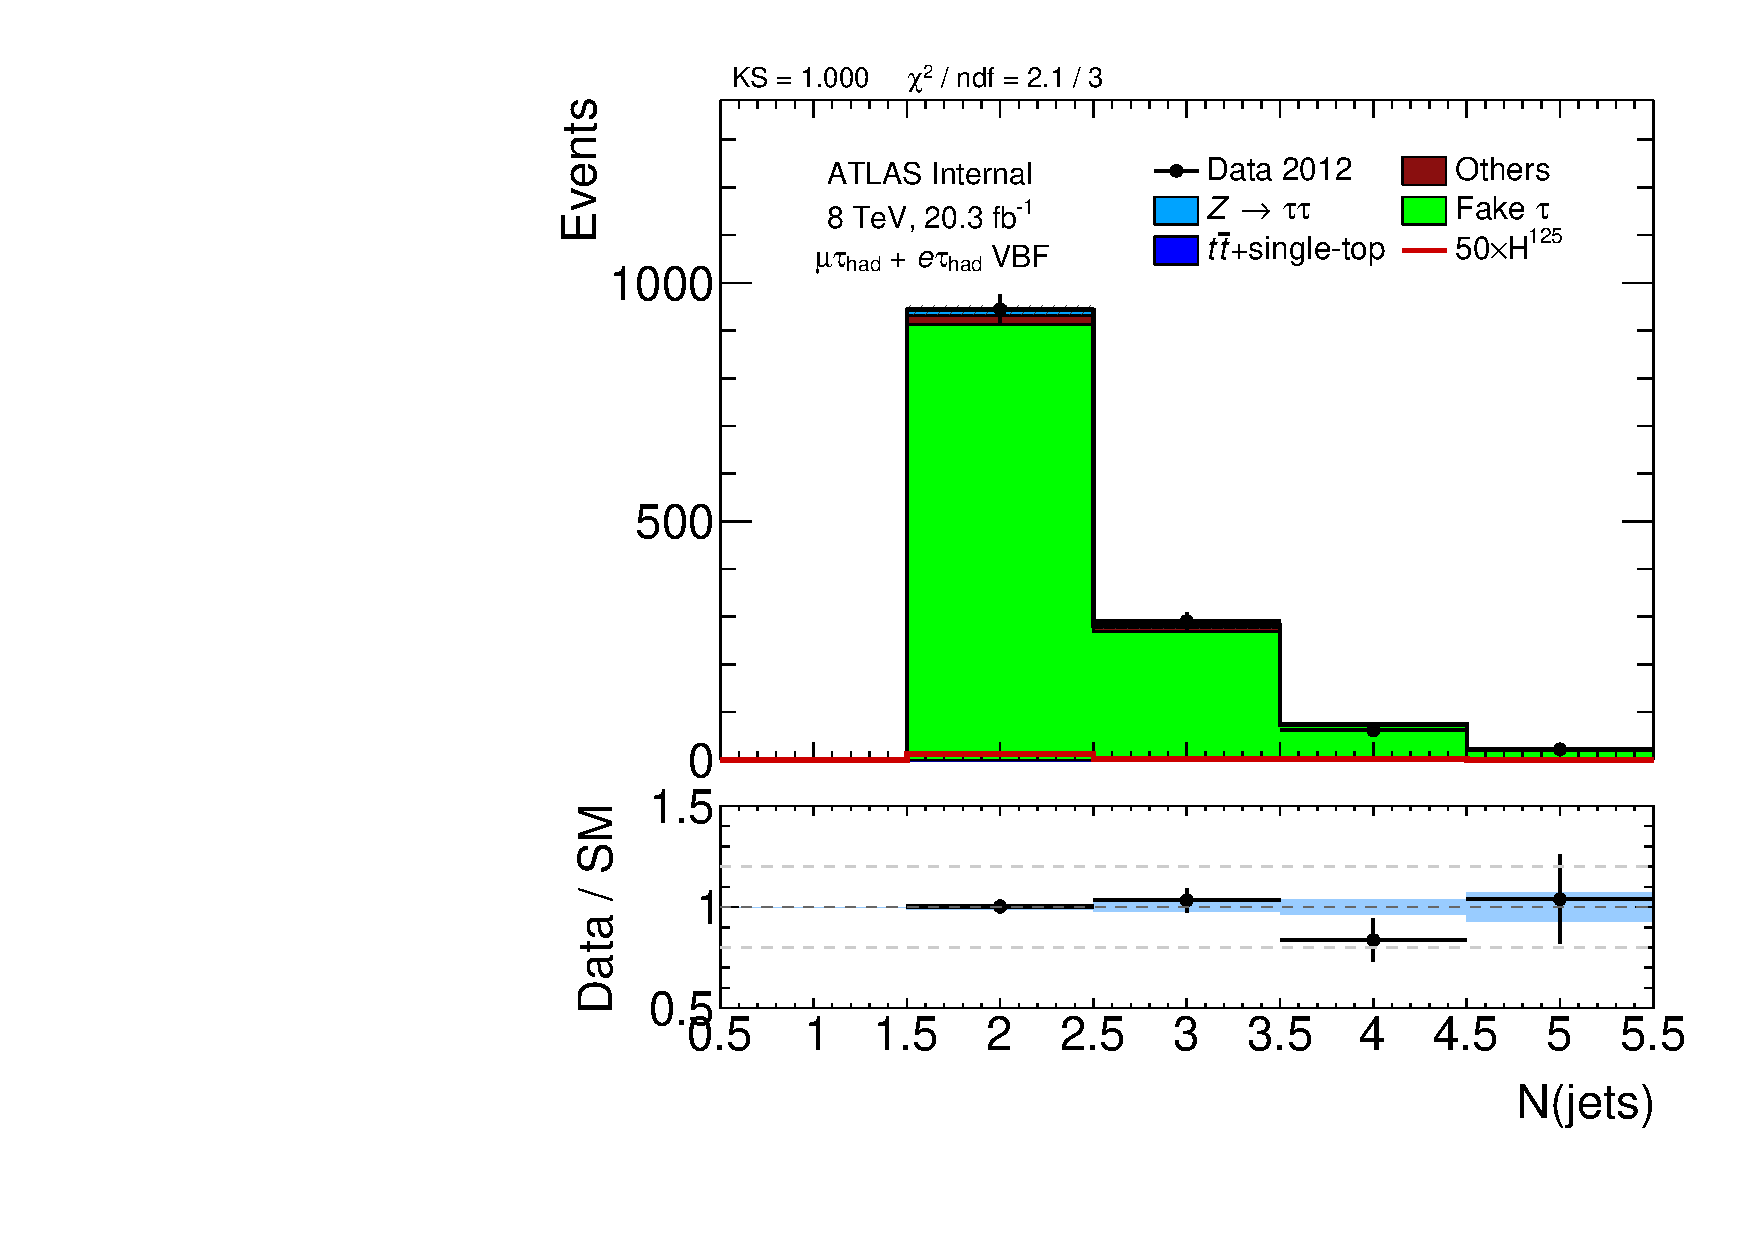
\includegraphics[width=0.32\textwidth]{figures/analysis/vbf-SSXCR/n-jets30}
  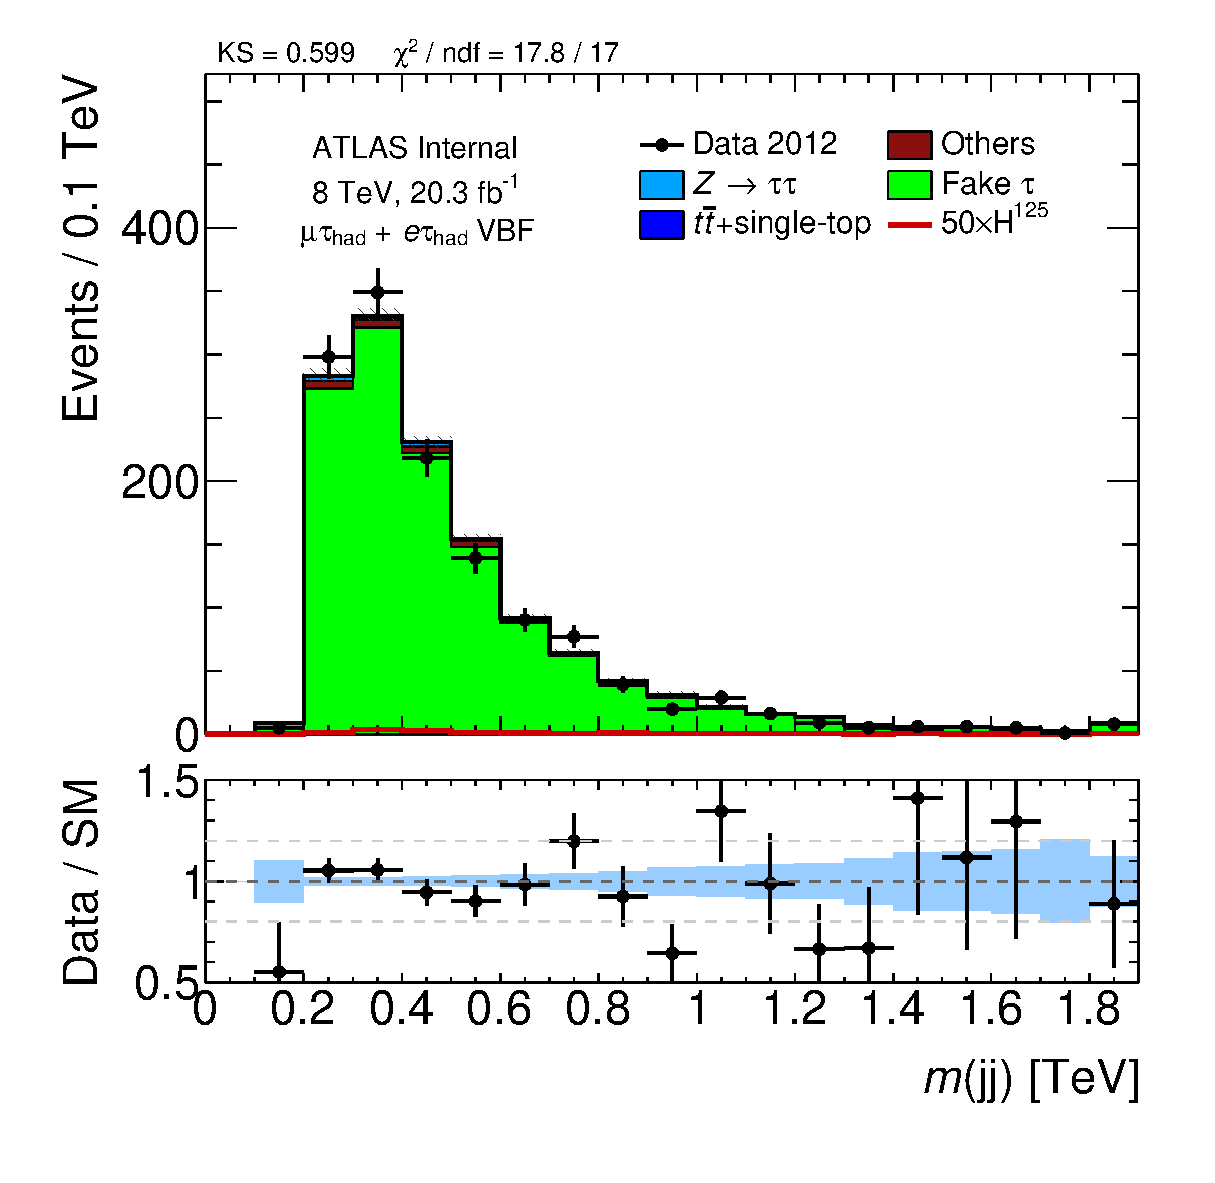
\includegraphics[width=0.32\textwidth]{figures/analysis/vbf-SSXCR/dijet-m-veryhigh}
  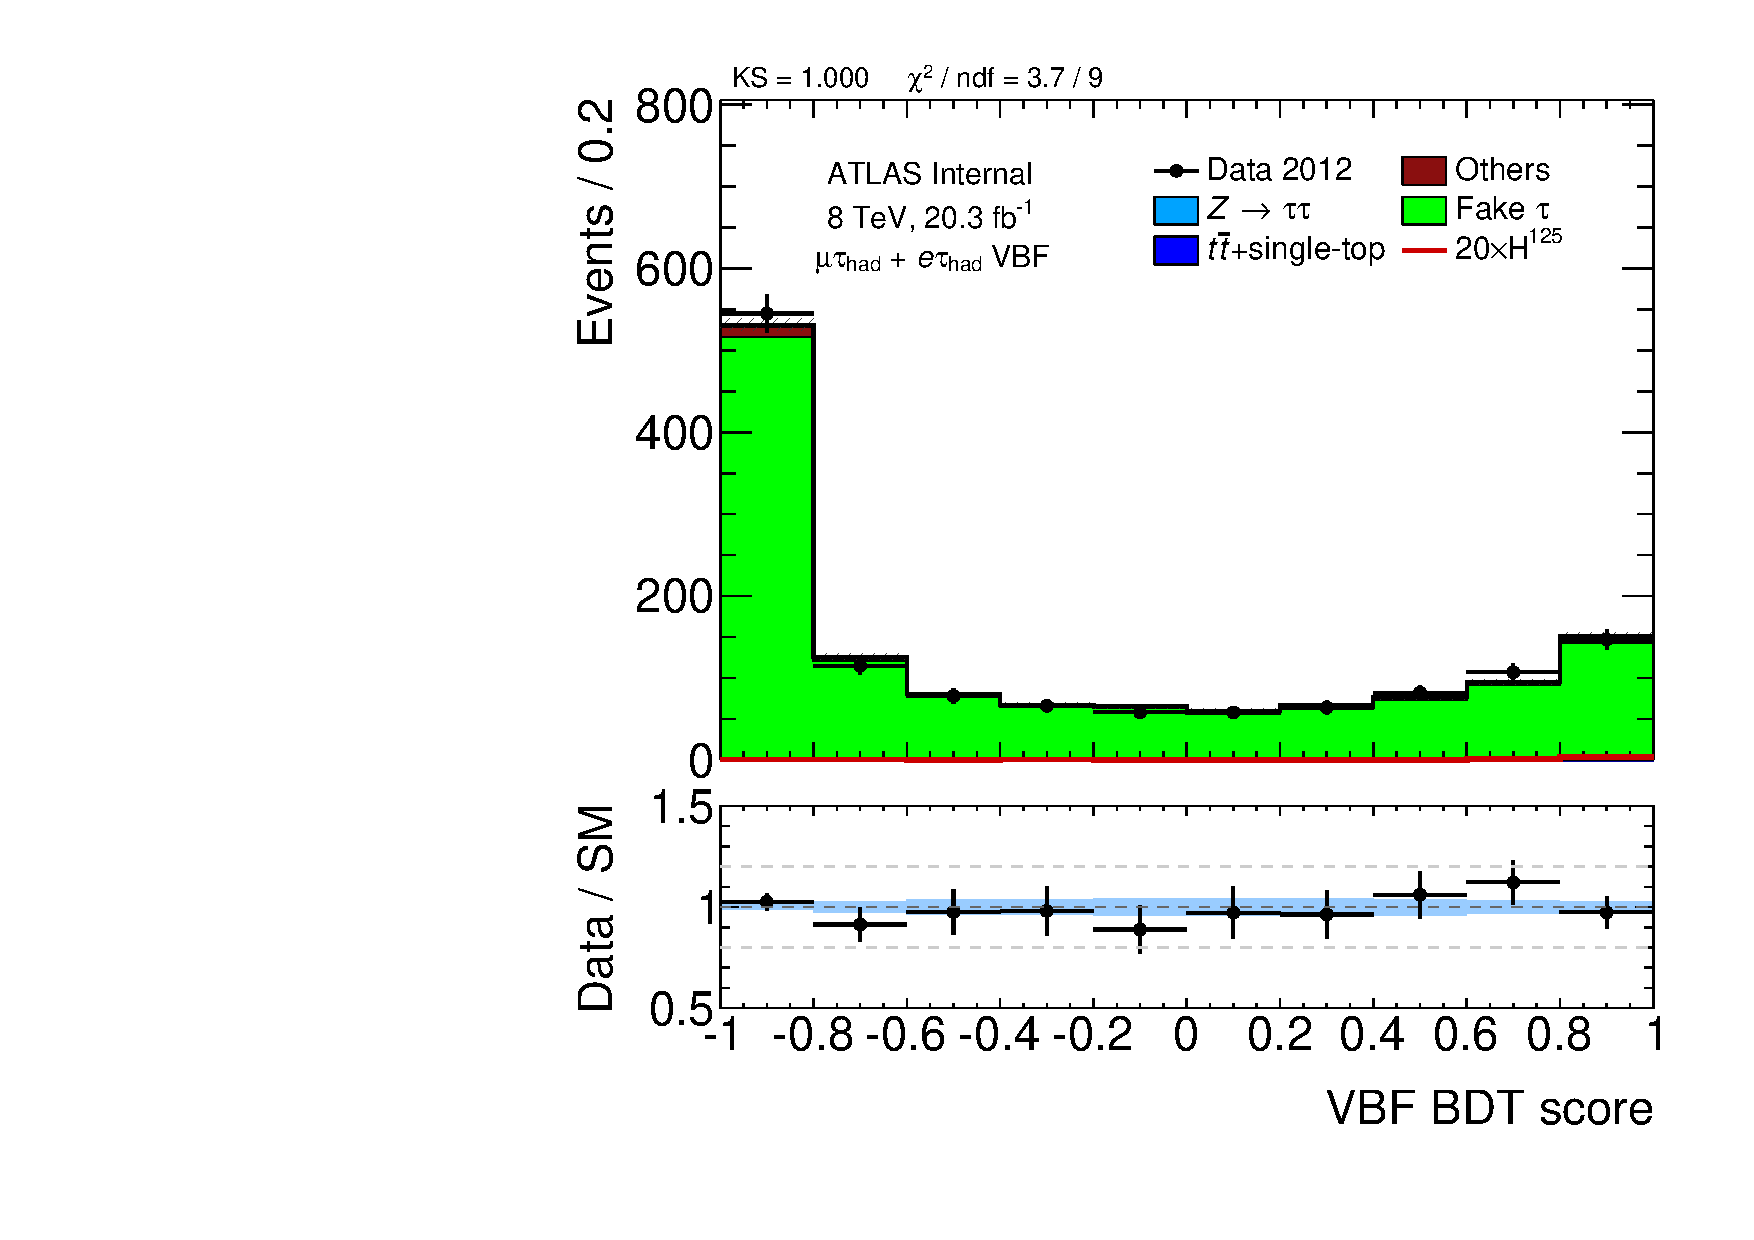
\includegraphics[width=0.32\textwidth]{figures/analysis/vbf-SSXCR/BDTEve-VBF} \\
  \caption{Comparison of data and $\fakes$ prediction in the same sign CR for various event kinematics. Only statistical uncertainties are shown.}
  \label{fig:backgrounds-SSXCR-jets}
\end{figure}

% \clearpage

\section{MC SR}

\begin{figure}[tp]
  \centering
  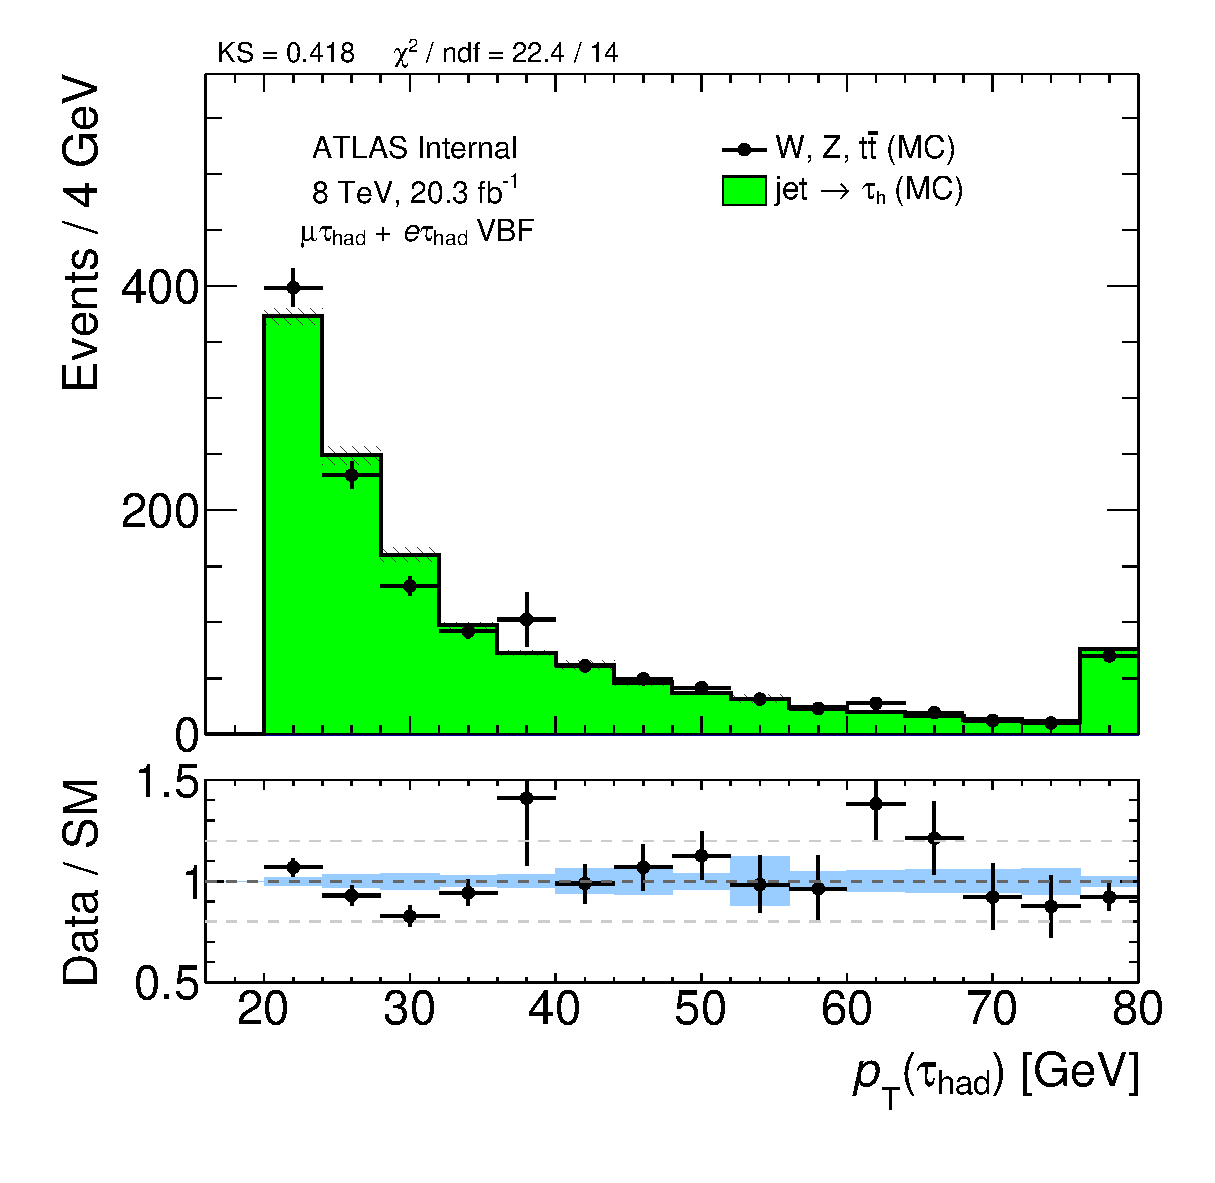
\includegraphics[width=0.32\textwidth]{figures/analysis/vbf-MCXSR/tau-pt}
  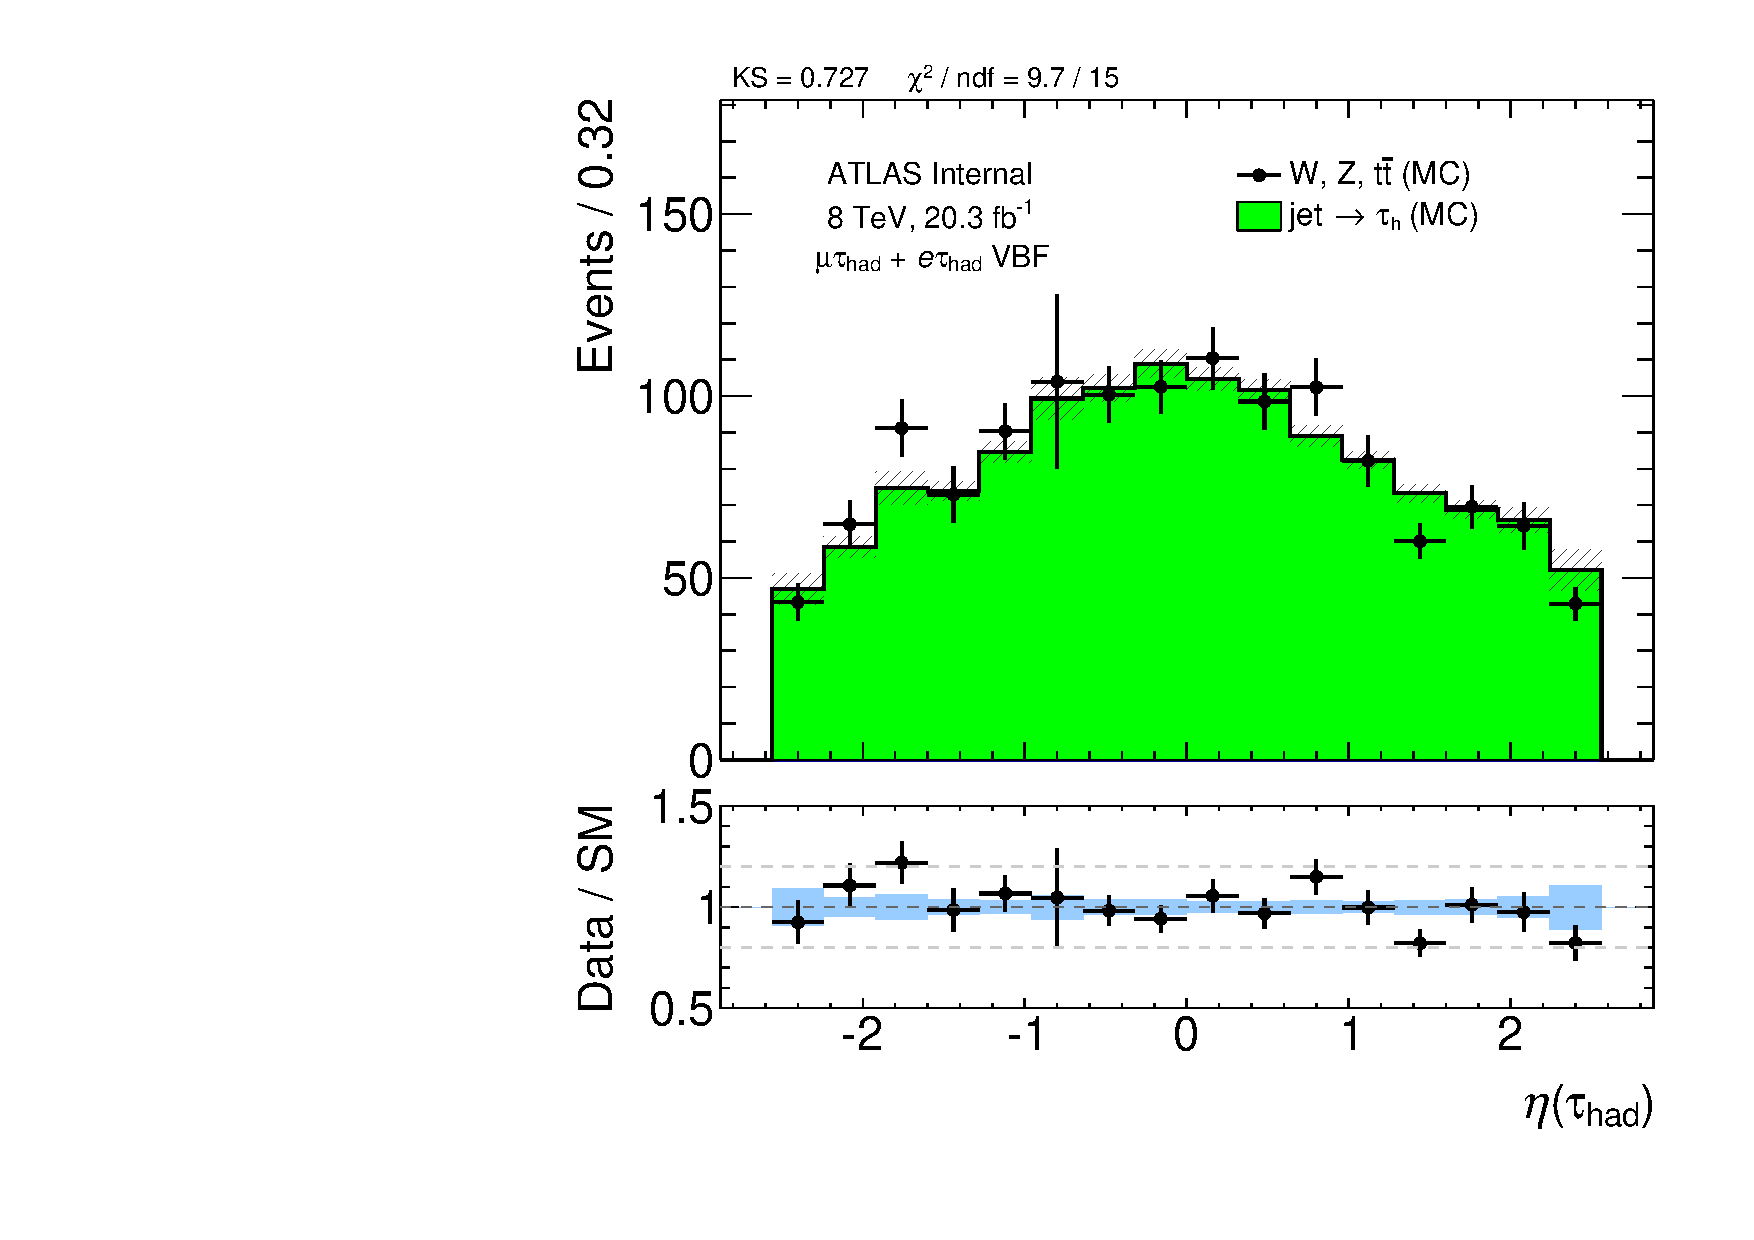
\includegraphics[width=0.32\textwidth]{figures/analysis/vbf-MCXSR/tau-eta}
  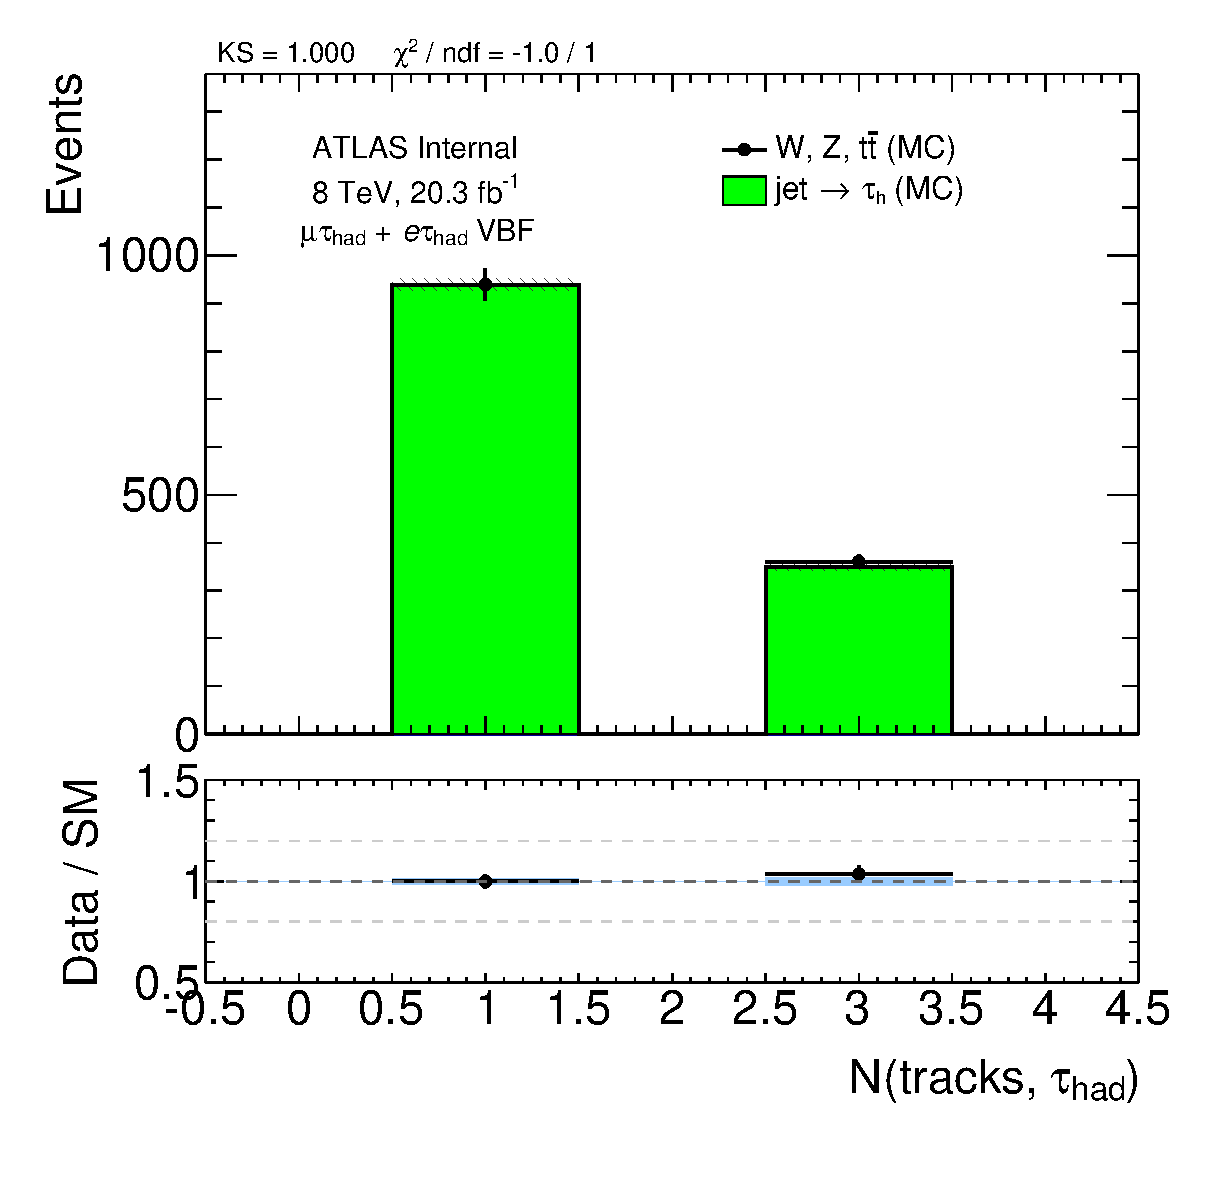
\includegraphics[width=0.32\textwidth]{figures/analysis/vbf-MCXSR/tau-numTrack} \\
  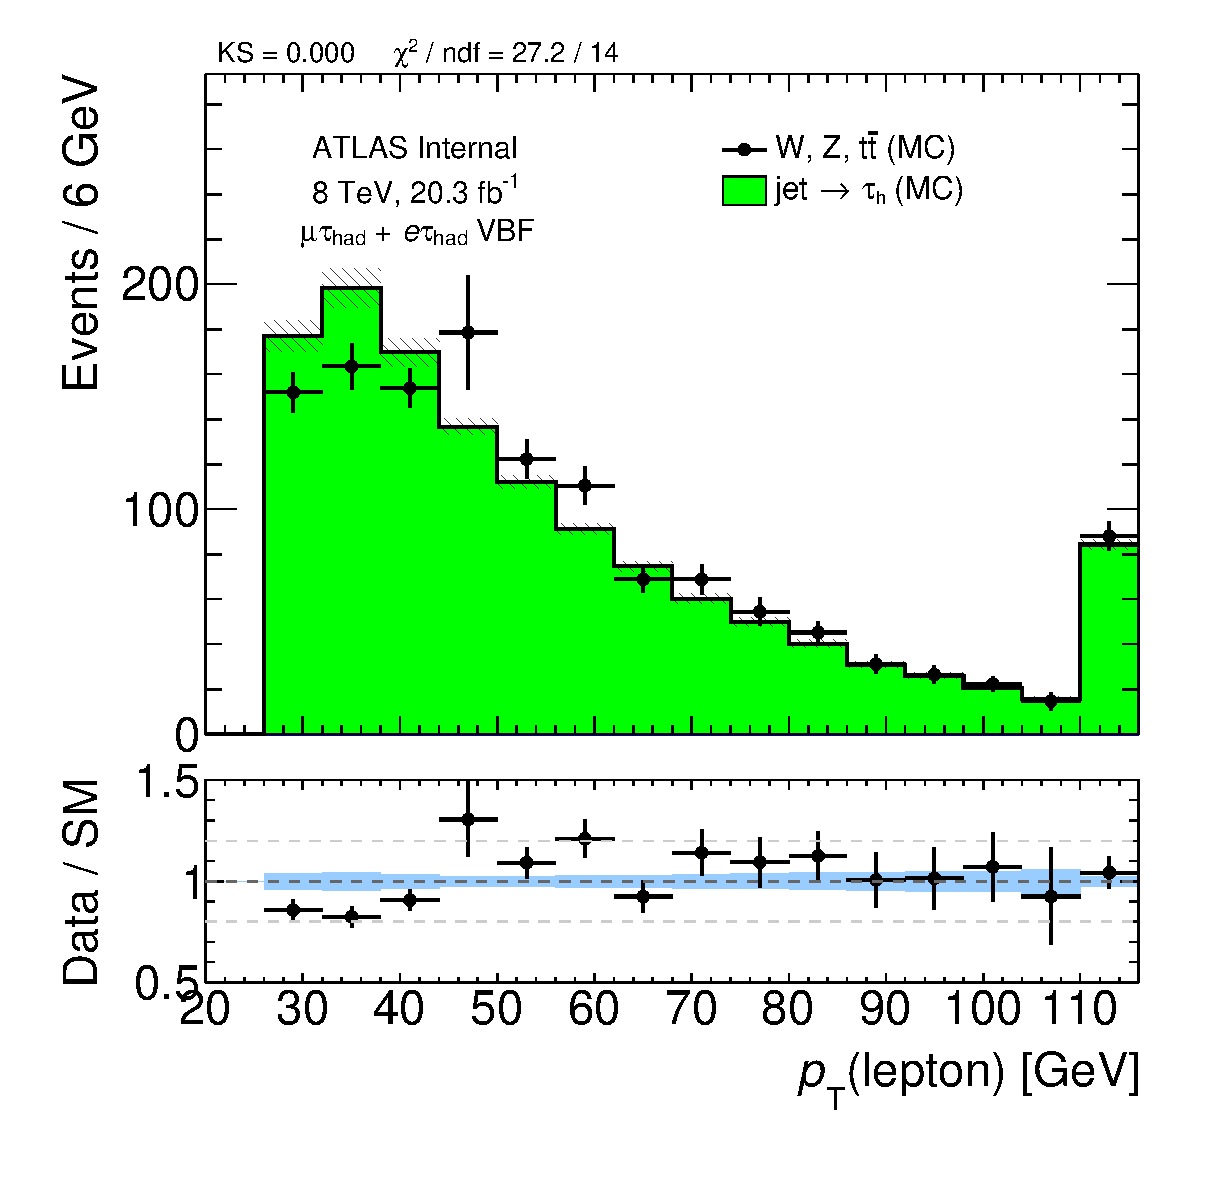
\includegraphics[width=0.32\textwidth]{figures/analysis/vbf-MCXSR/lep-pt-hi}
  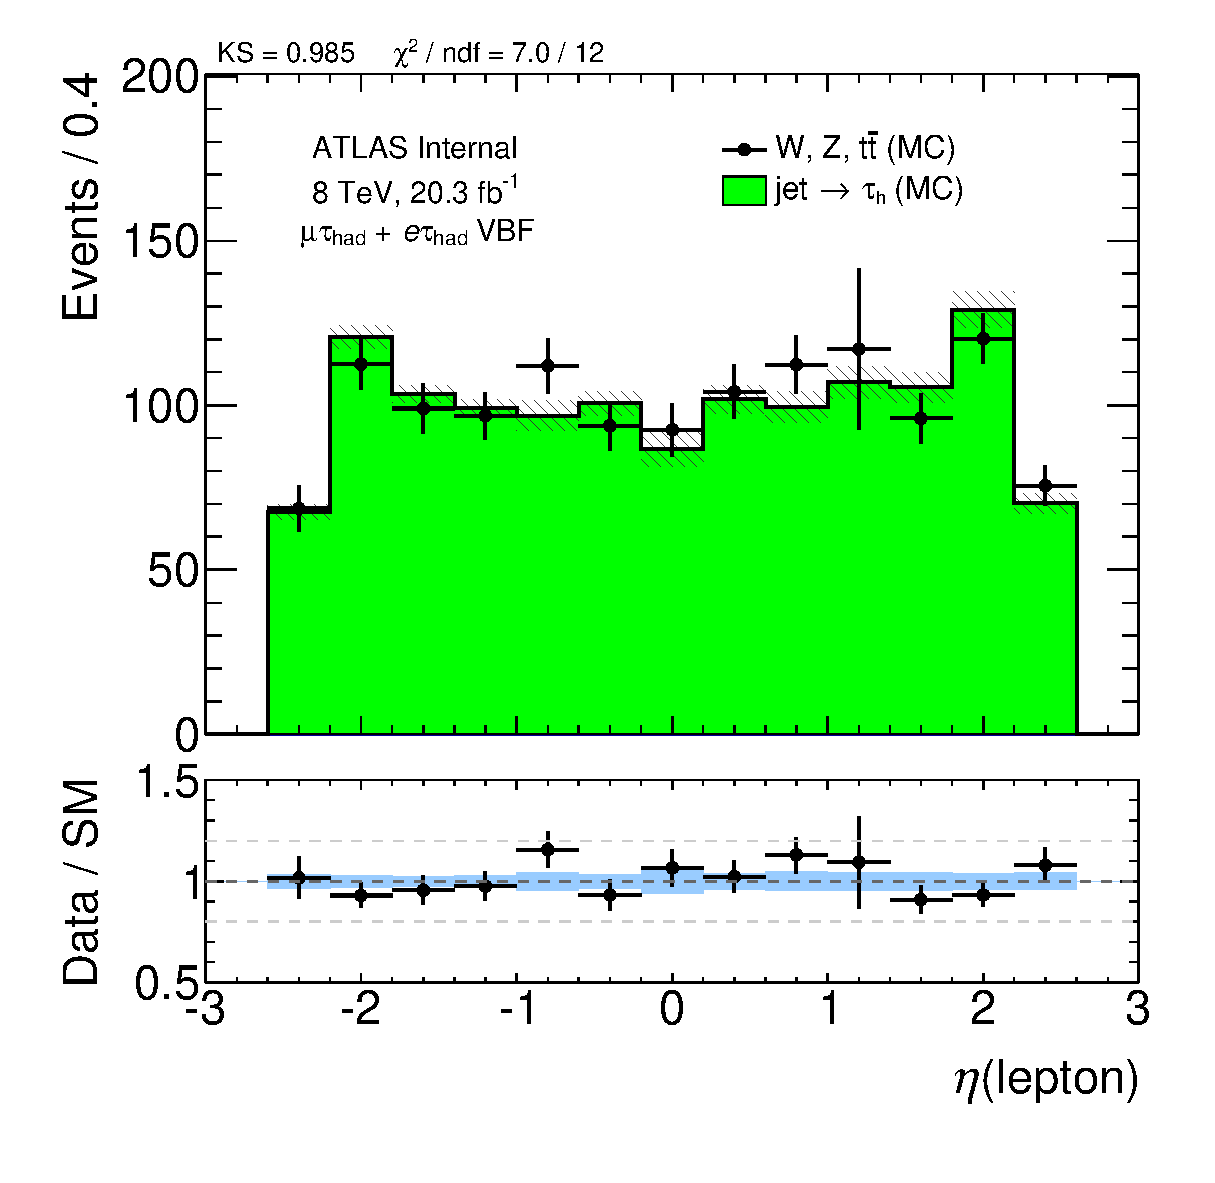
\includegraphics[width=0.32\textwidth]{figures/analysis/vbf-MCXSR/lep-eta}
  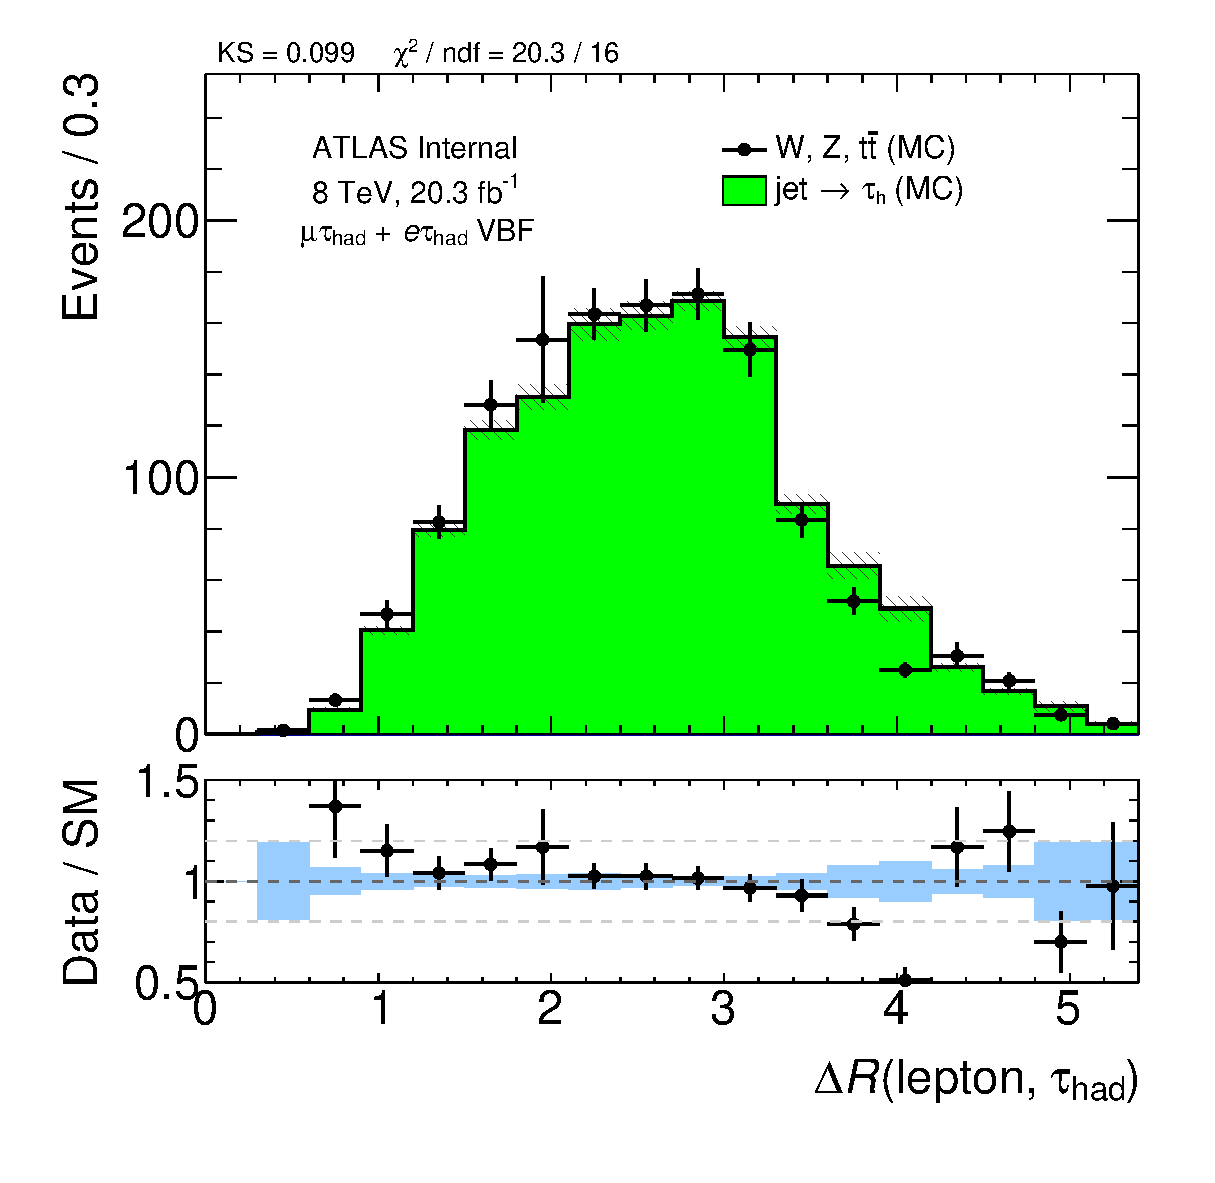
\includegraphics[width=0.32\textwidth]{figures/analysis/vbf-MCXSR/taulep-dR} \\
  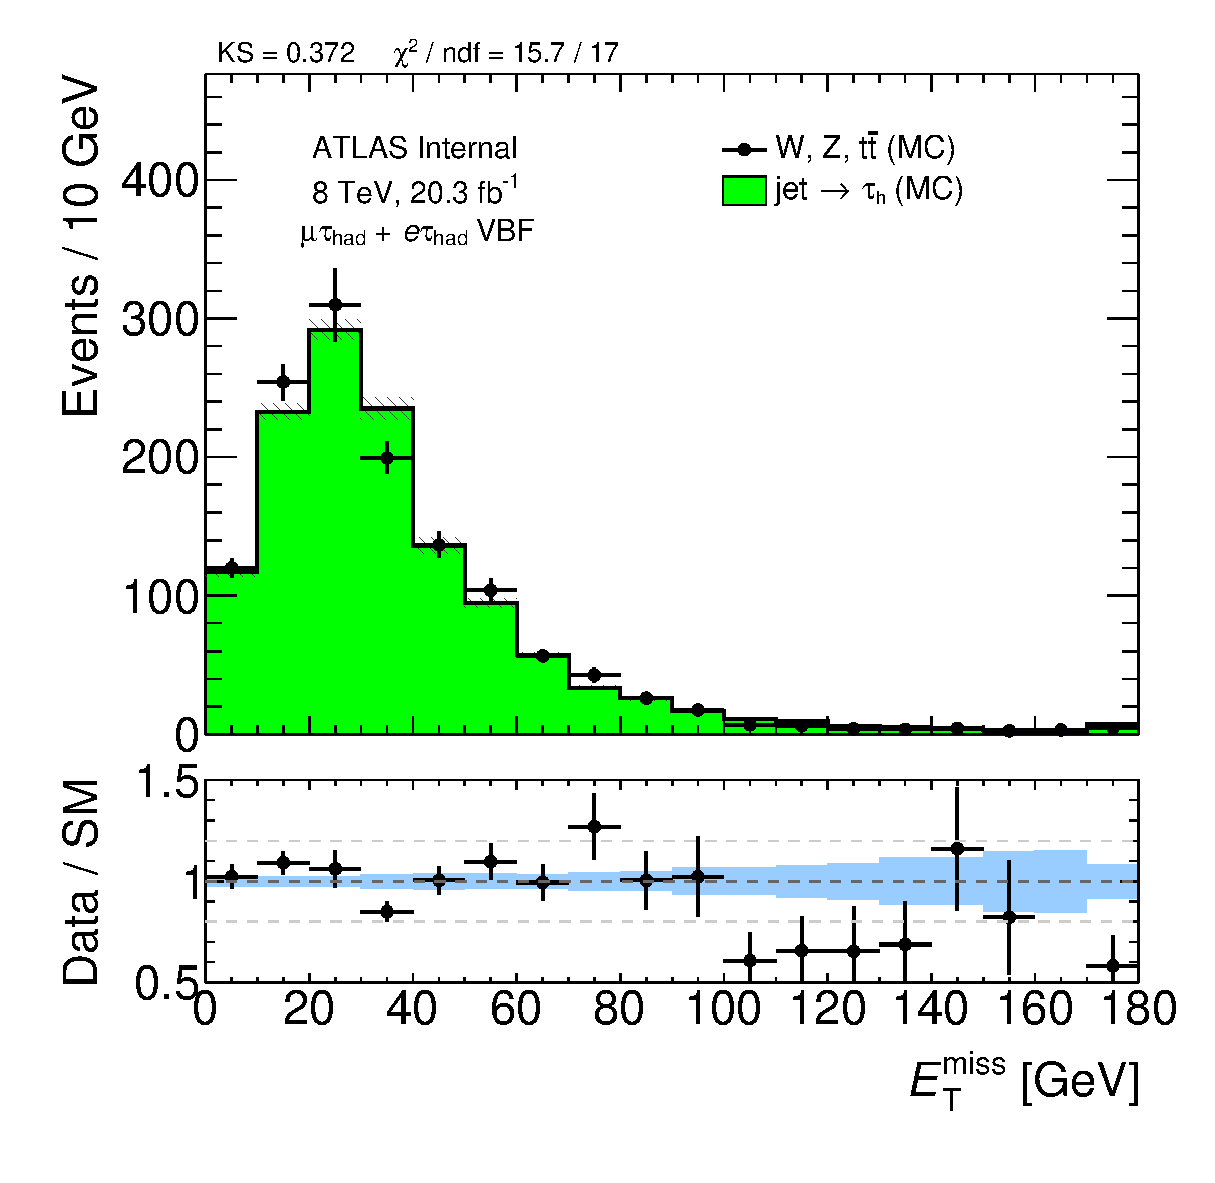
\includegraphics[width=0.32\textwidth]{figures/analysis/vbf-MCXSR/met-pt-hi}
  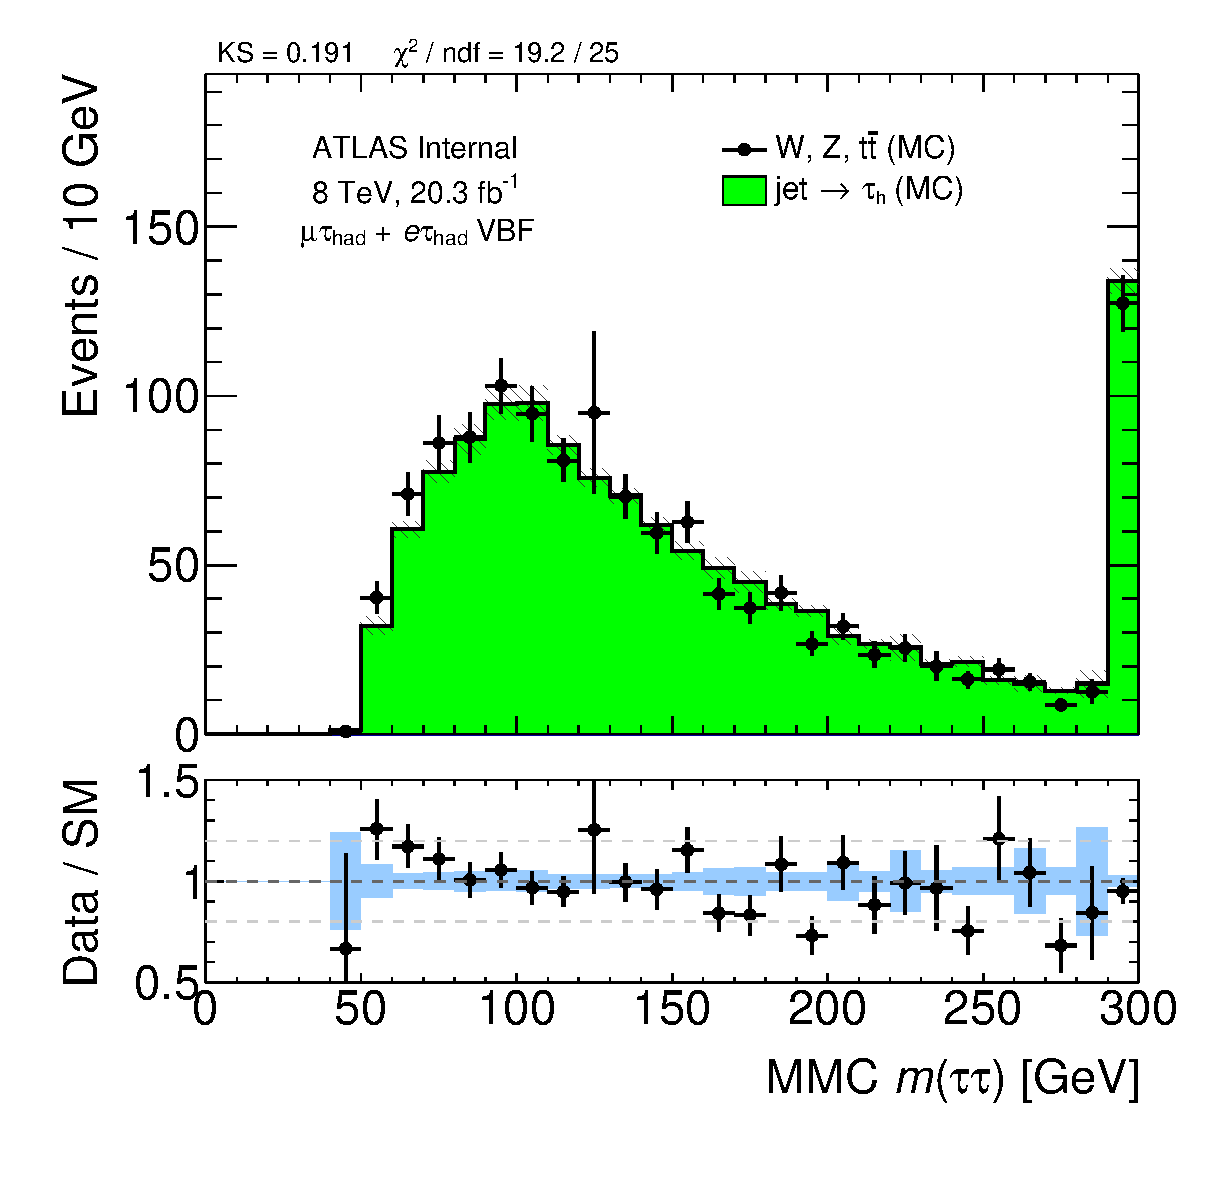
\includegraphics[width=0.32\textwidth]{figures/analysis/vbf-MCXSR/mMMC}
  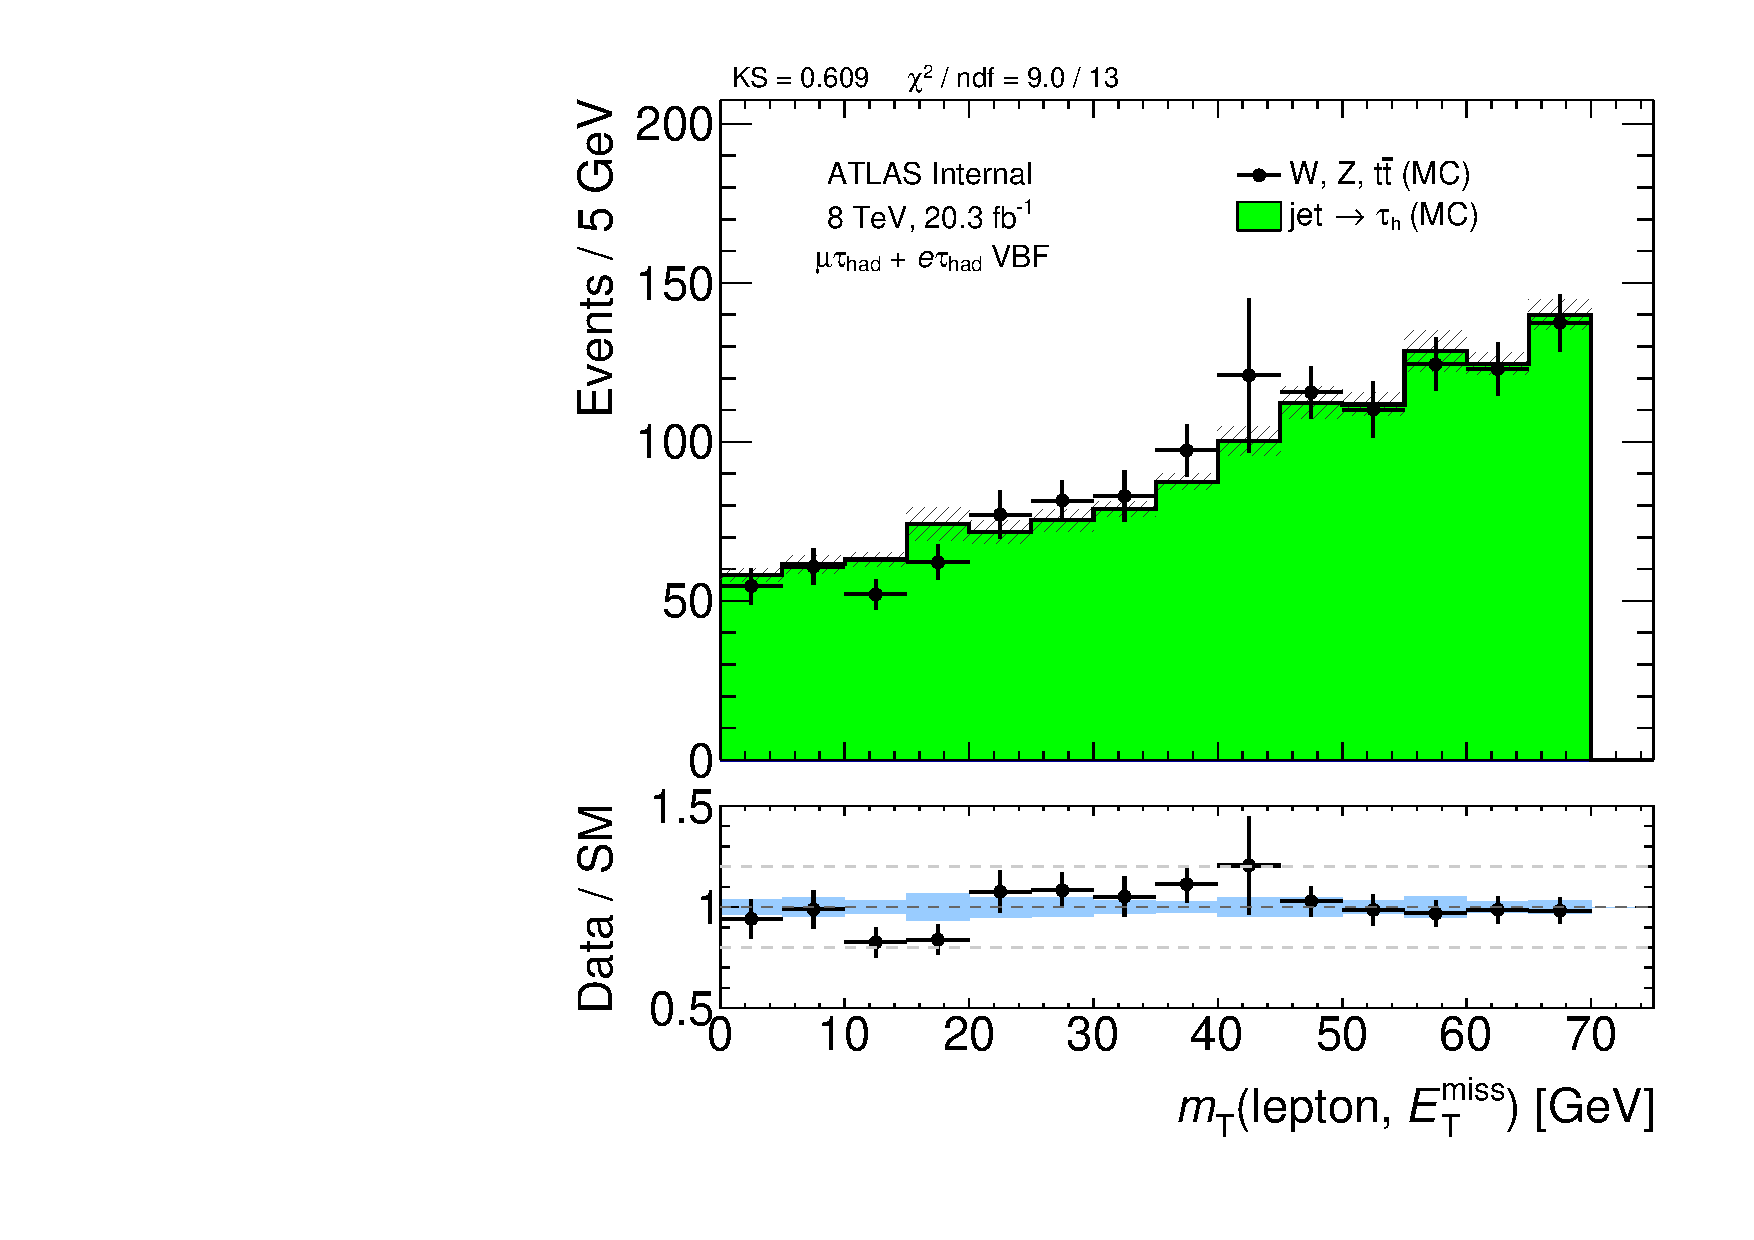
\includegraphics[width=0.32\textwidth]{figures/analysis/vbf-MCXSR/mT} \\
  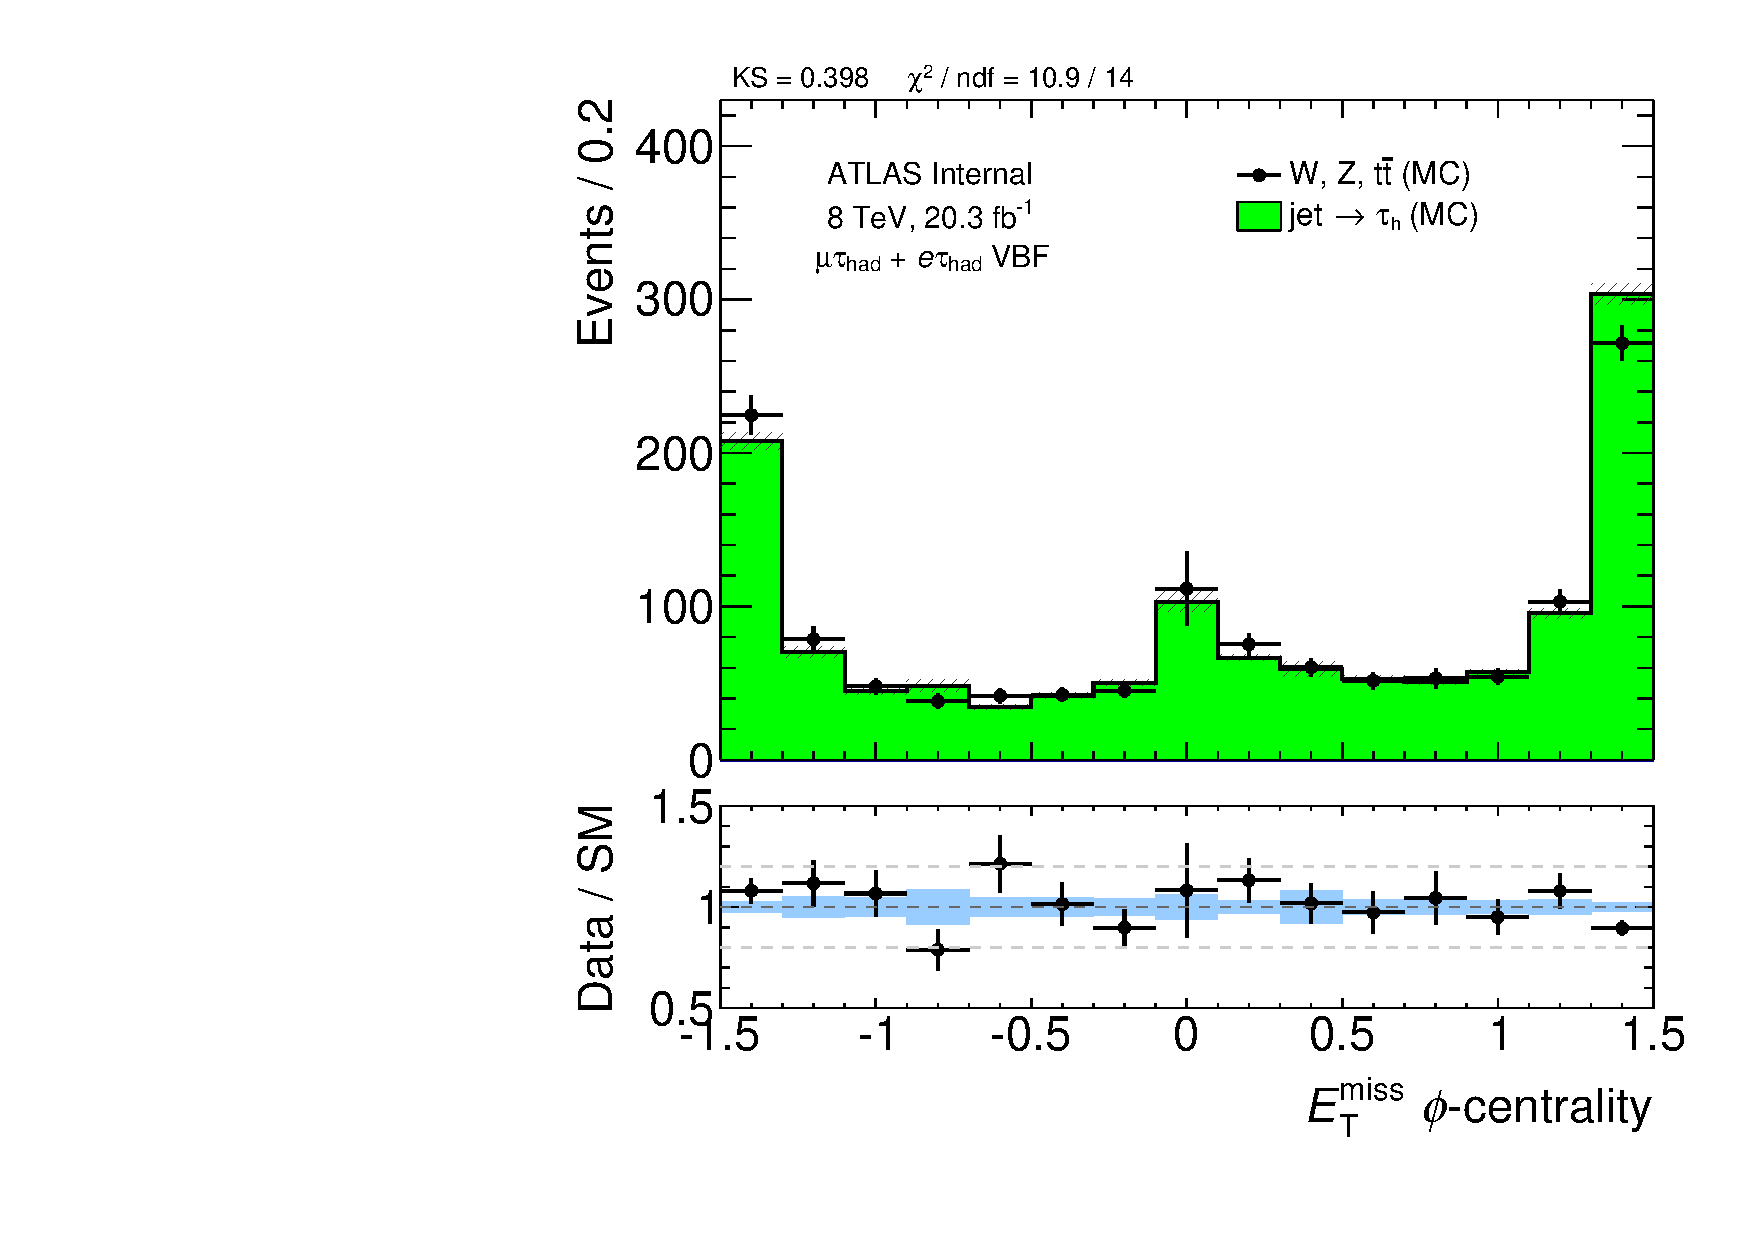
\includegraphics[width=0.32\textwidth]{figures/analysis/vbf-MCXSR/met-phi-centrality}
  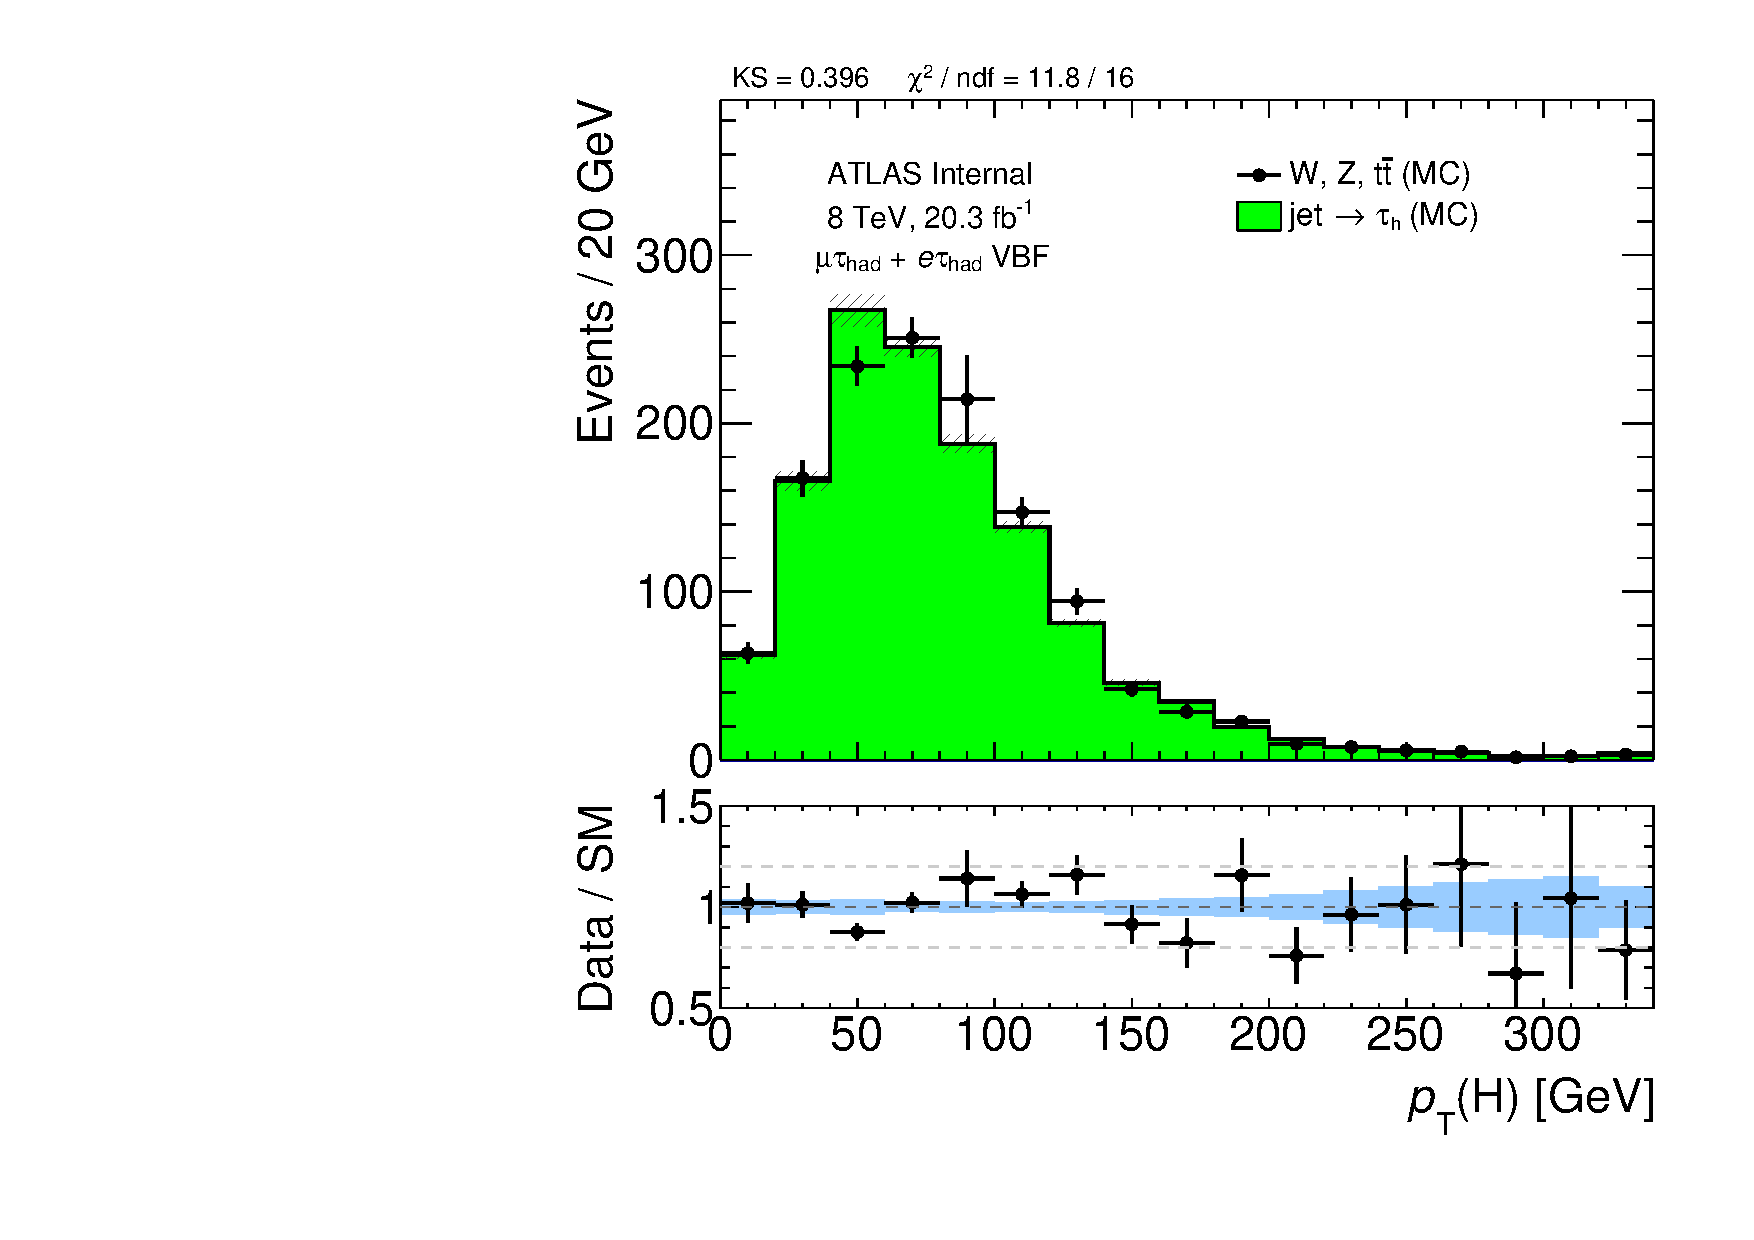
\includegraphics[width=0.32\textwidth]{figures/analysis/vbf-MCXSR/H-pt-hi}
  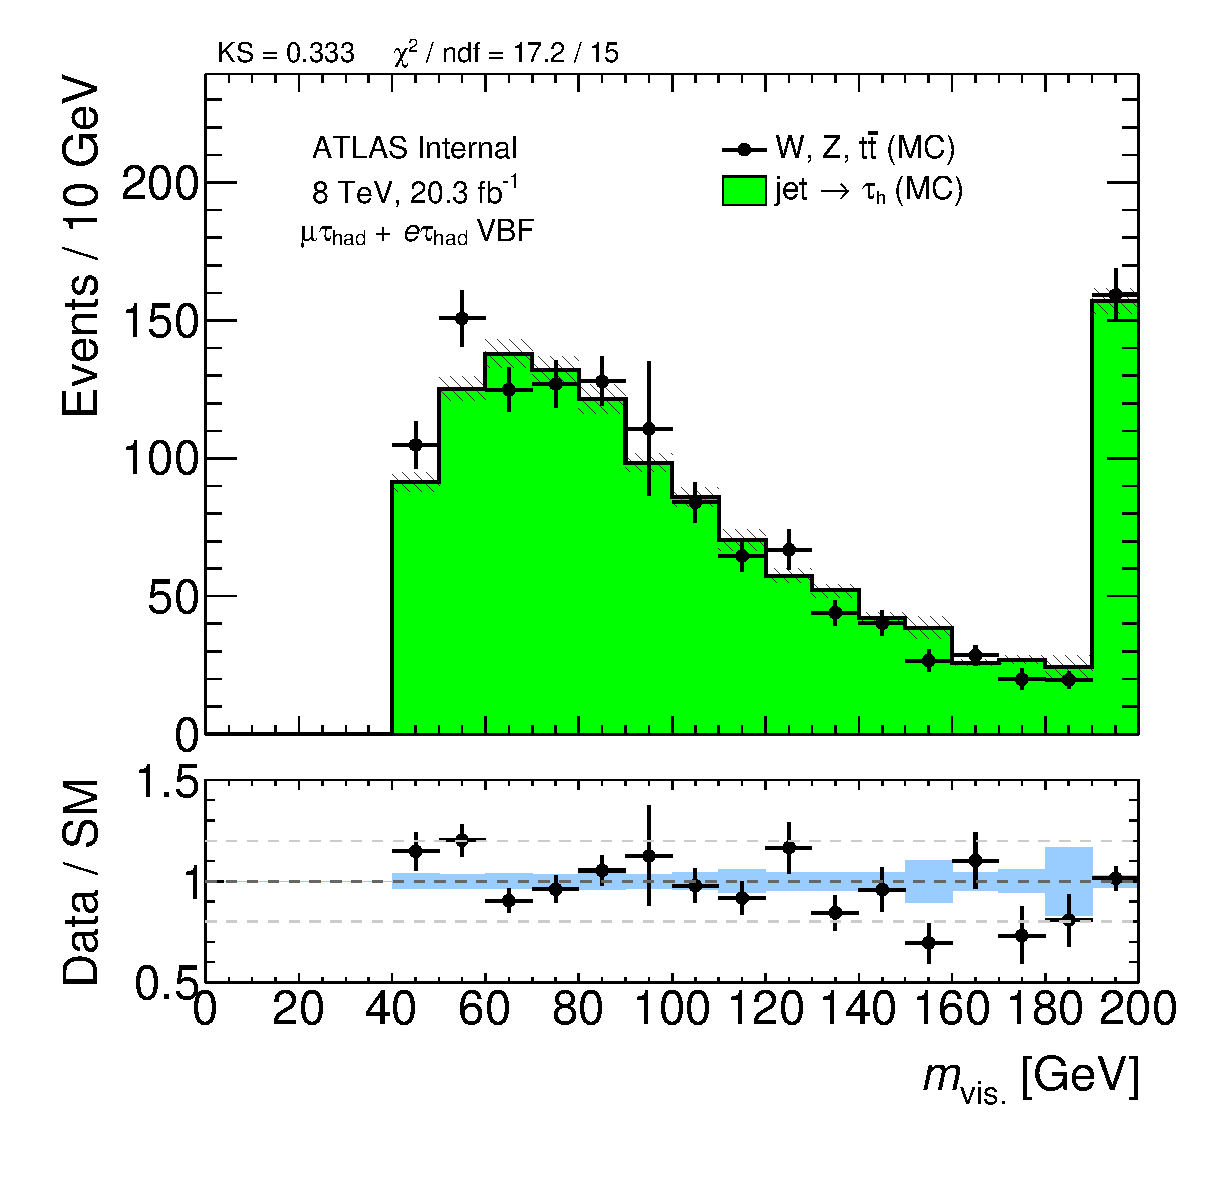
\includegraphics[width=0.32\textwidth]{figures/analysis/vbf-MCXSR/mvis} \\
  \caption{Comparison of the prediction of identified taus and the $\fakes$ prediction, both in simulation, in the signal region for various event kinematics. Only statistical uncertainties are shown.}
  \label{fig:backgrounds-MCXSR-taus}
\end{figure}

\begin{figure}[tp]
  \centering
  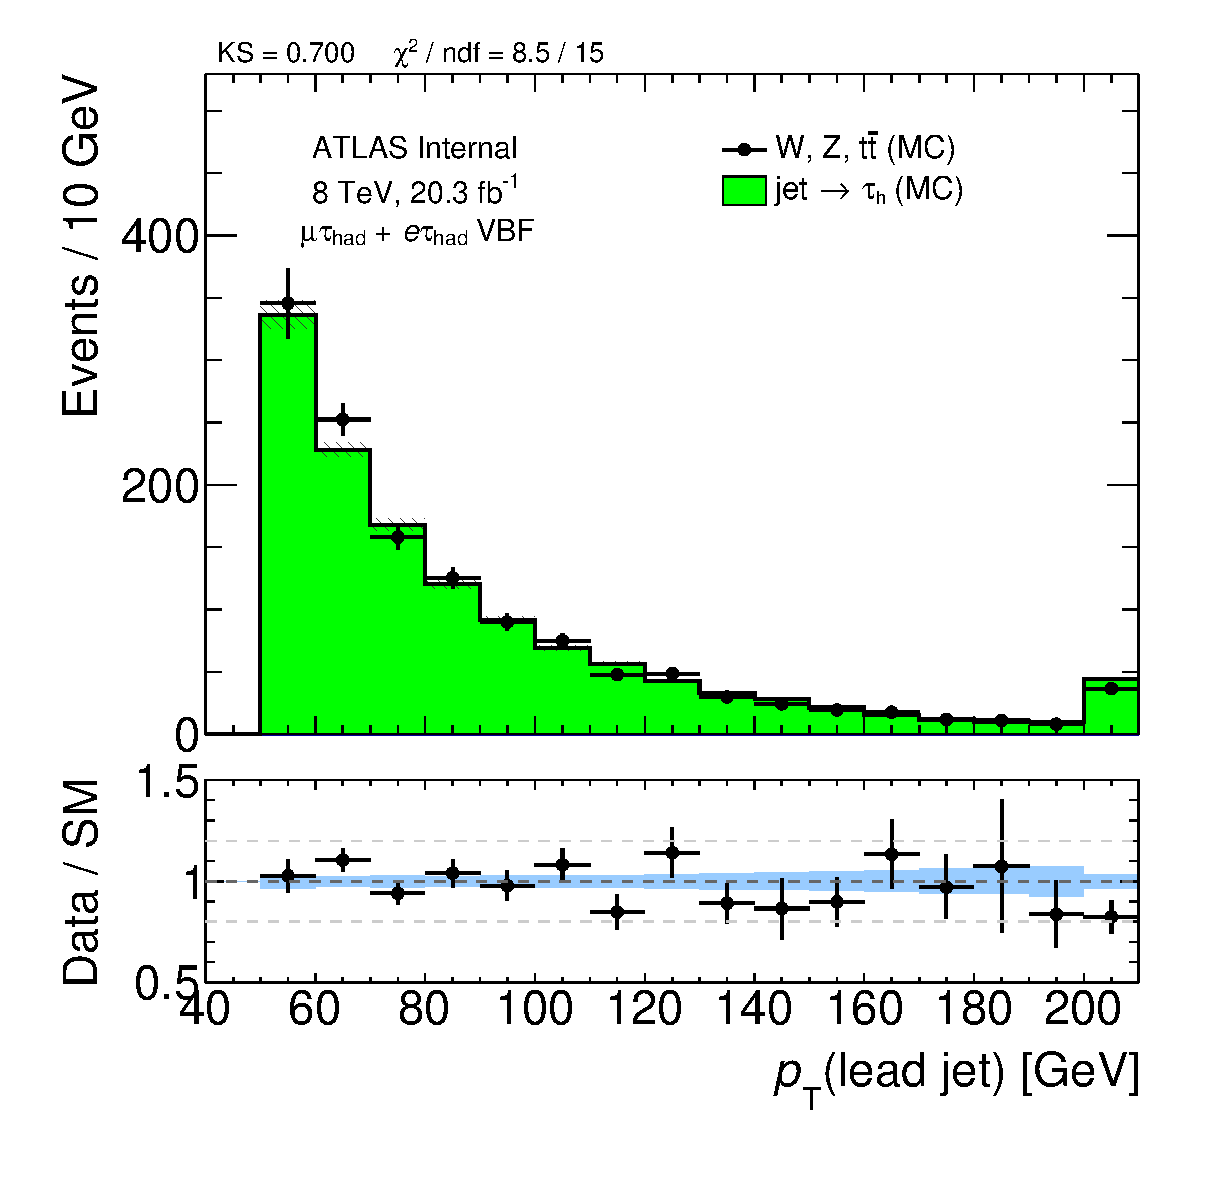
\includegraphics[width=0.32\textwidth]{figures/analysis/vbf-MCXSR/jet-1-pt}
  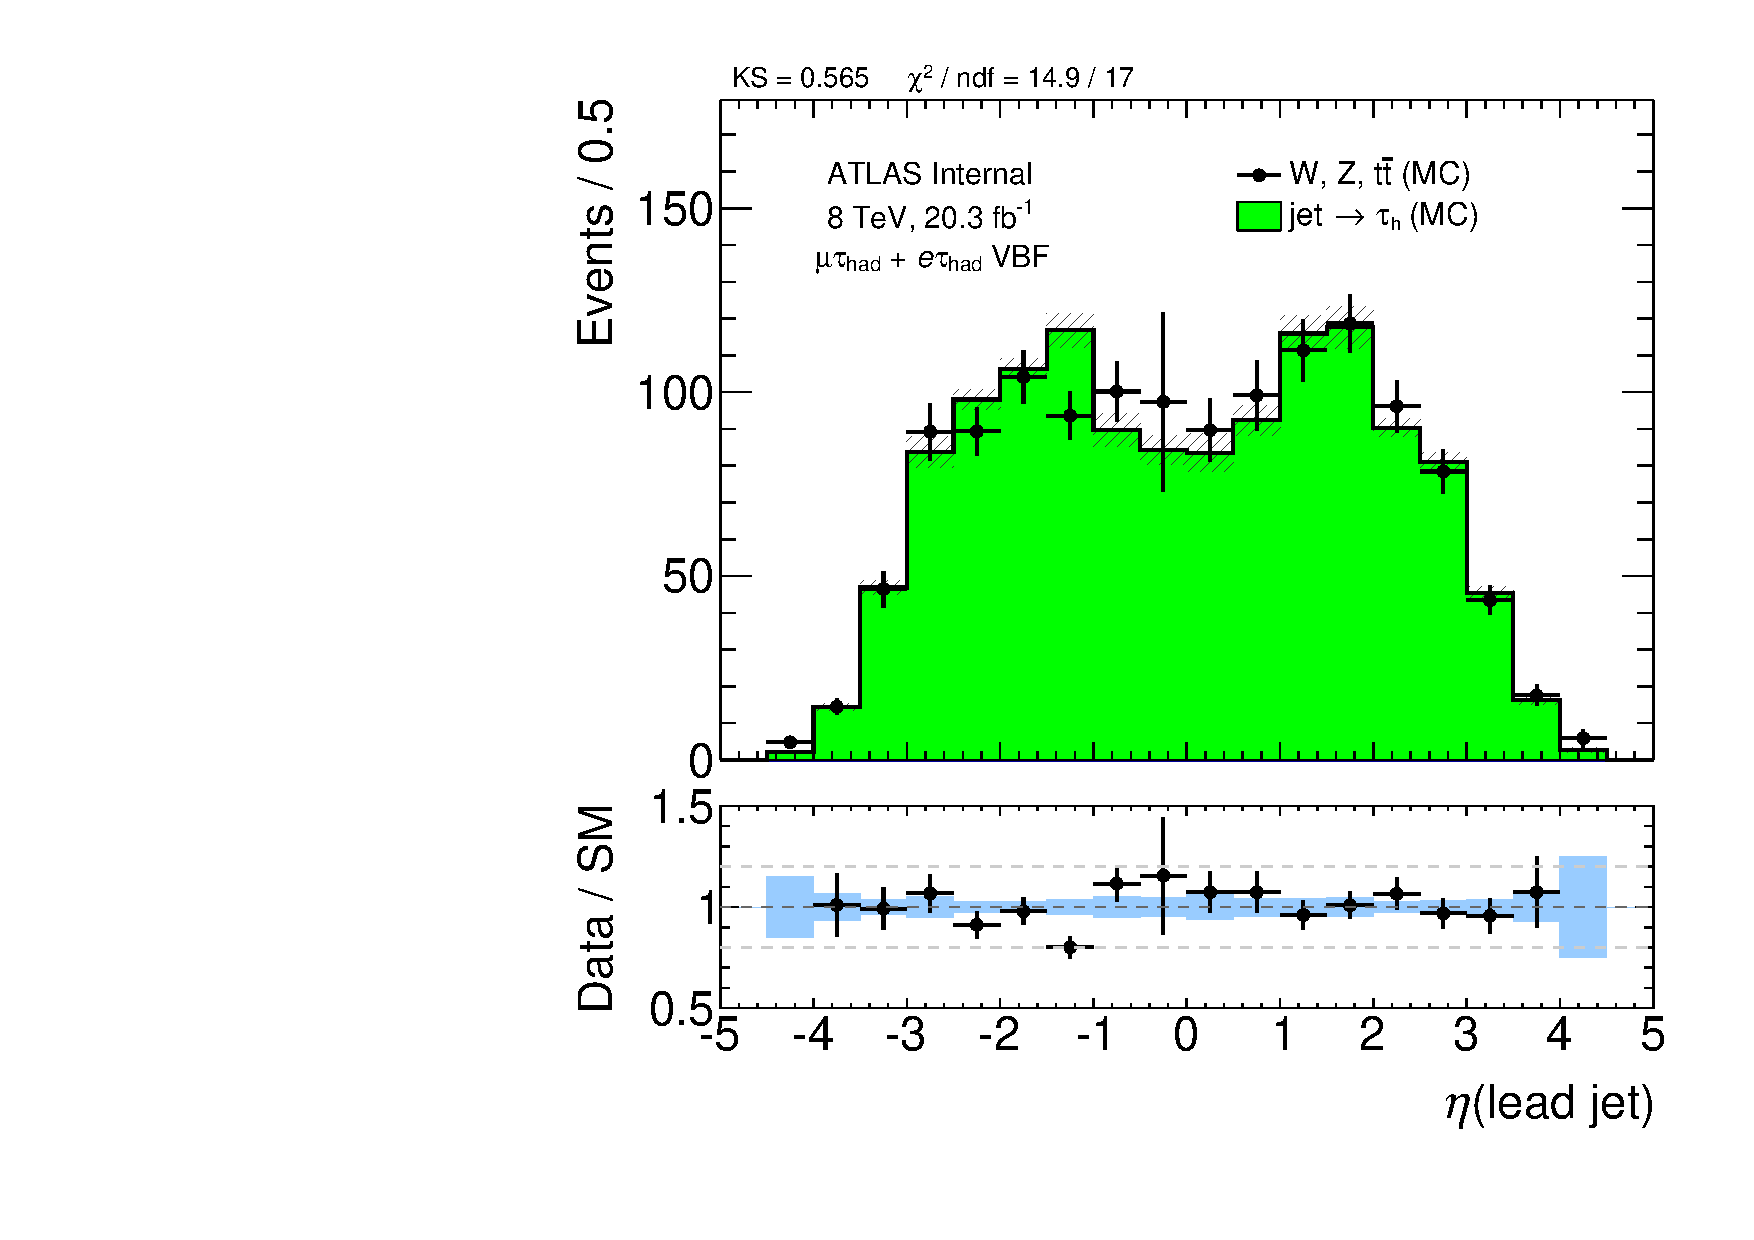
\includegraphics[width=0.32\textwidth]{figures/analysis/vbf-MCXSR/jet-1-eta}
  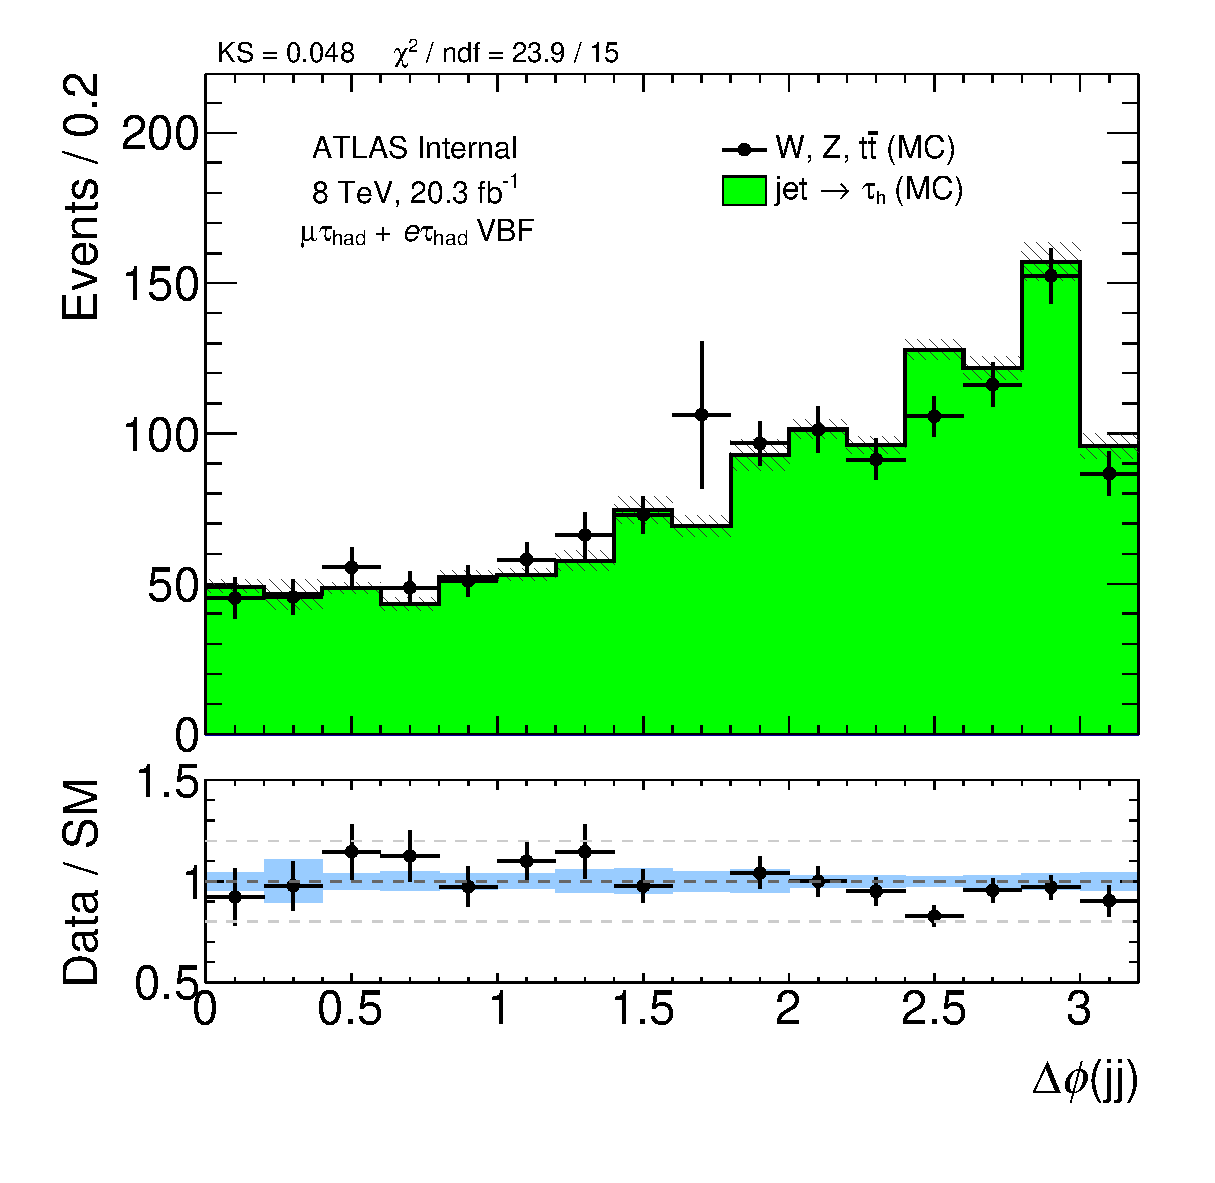
\includegraphics[width=0.32\textwidth]{figures/analysis/vbf-MCXSR/jets-dphi} \\
  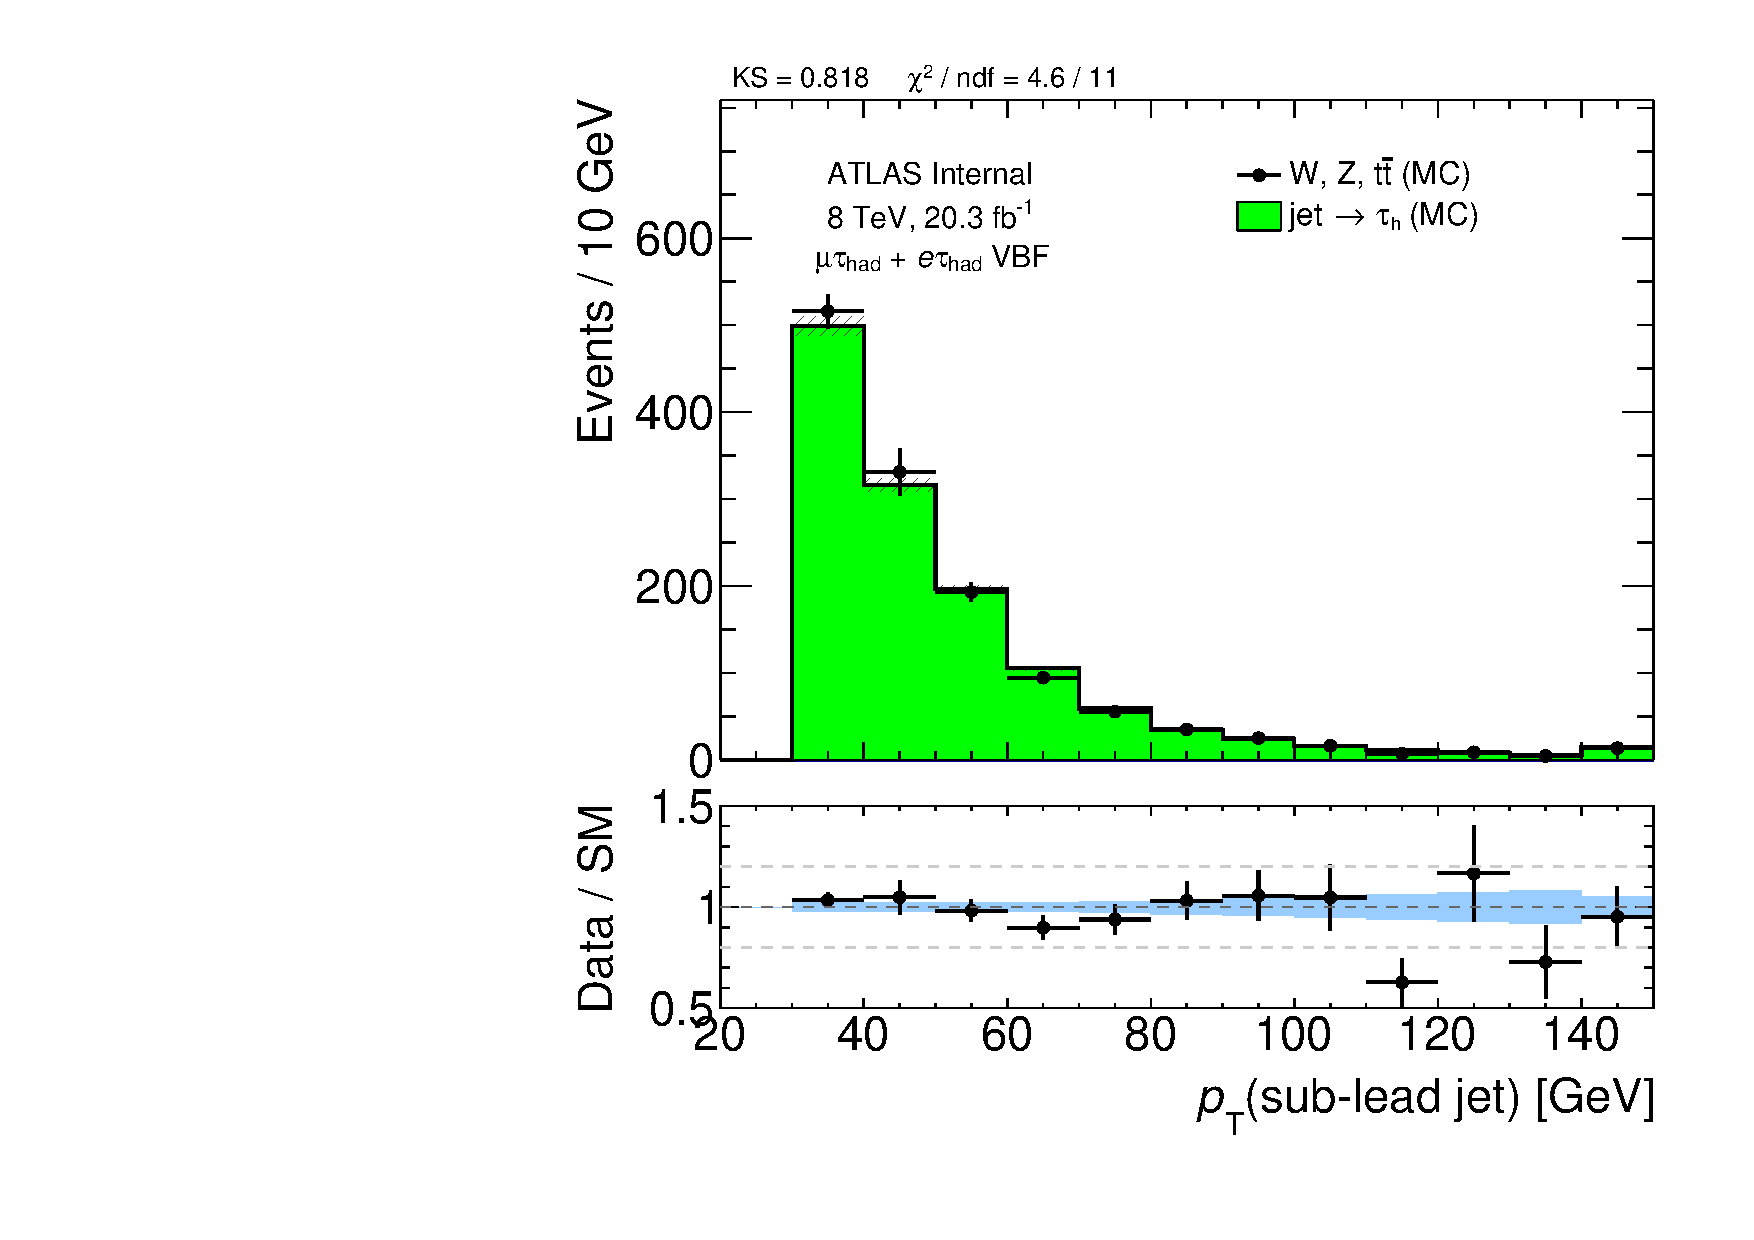
\includegraphics[width=0.32\textwidth]{figures/analysis/vbf-MCXSR/jet-2-pt}
  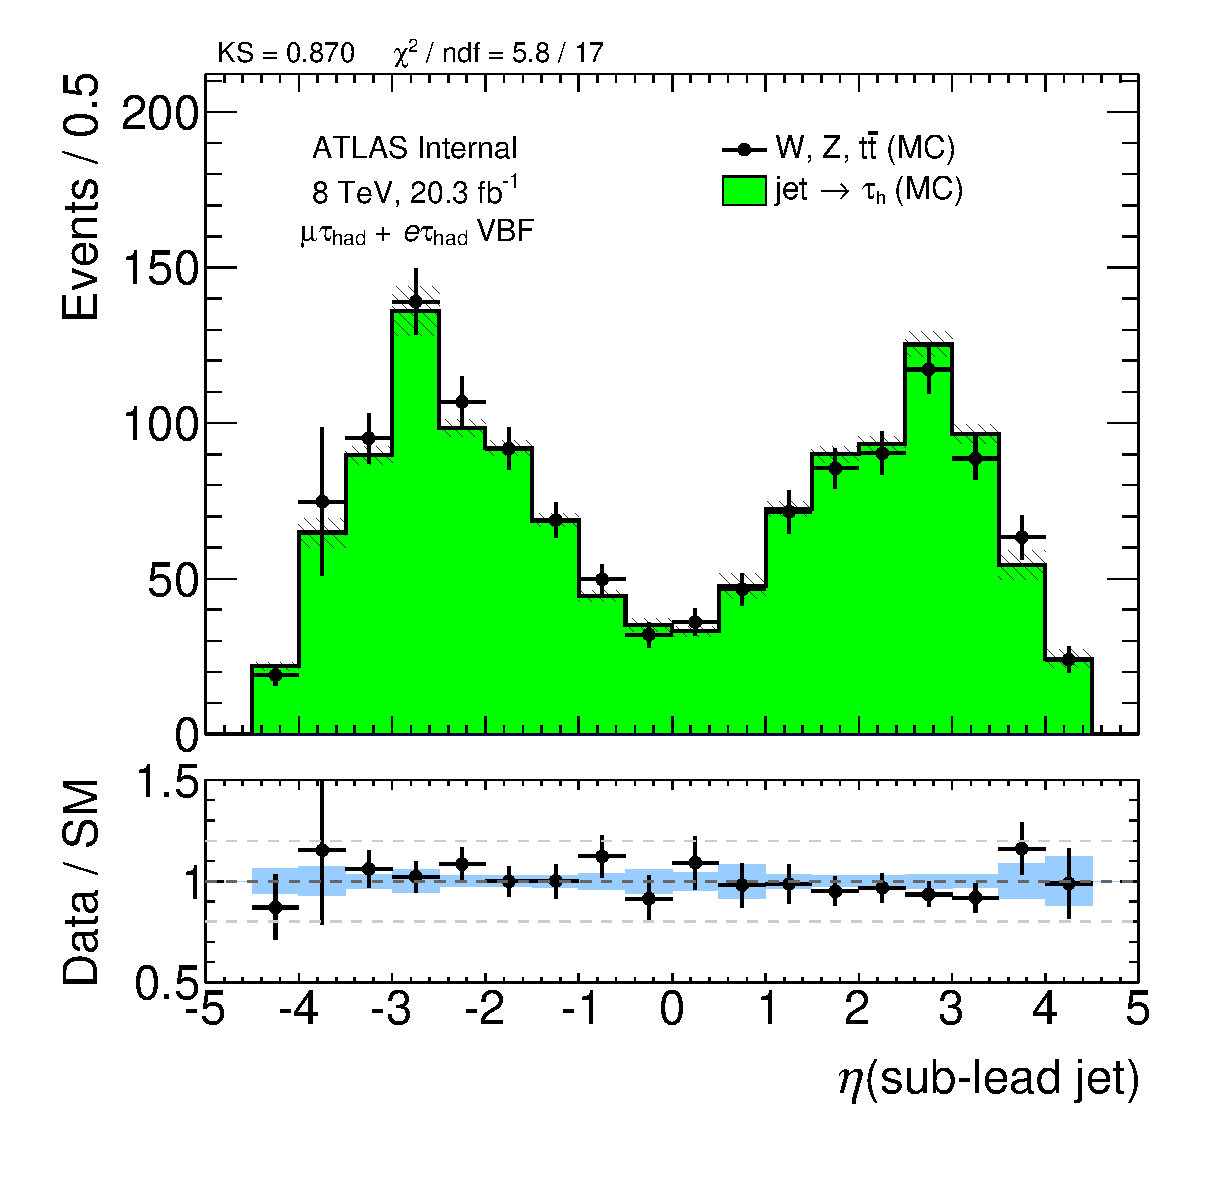
\includegraphics[width=0.32\textwidth]{figures/analysis/vbf-MCXSR/jet-2-eta}
  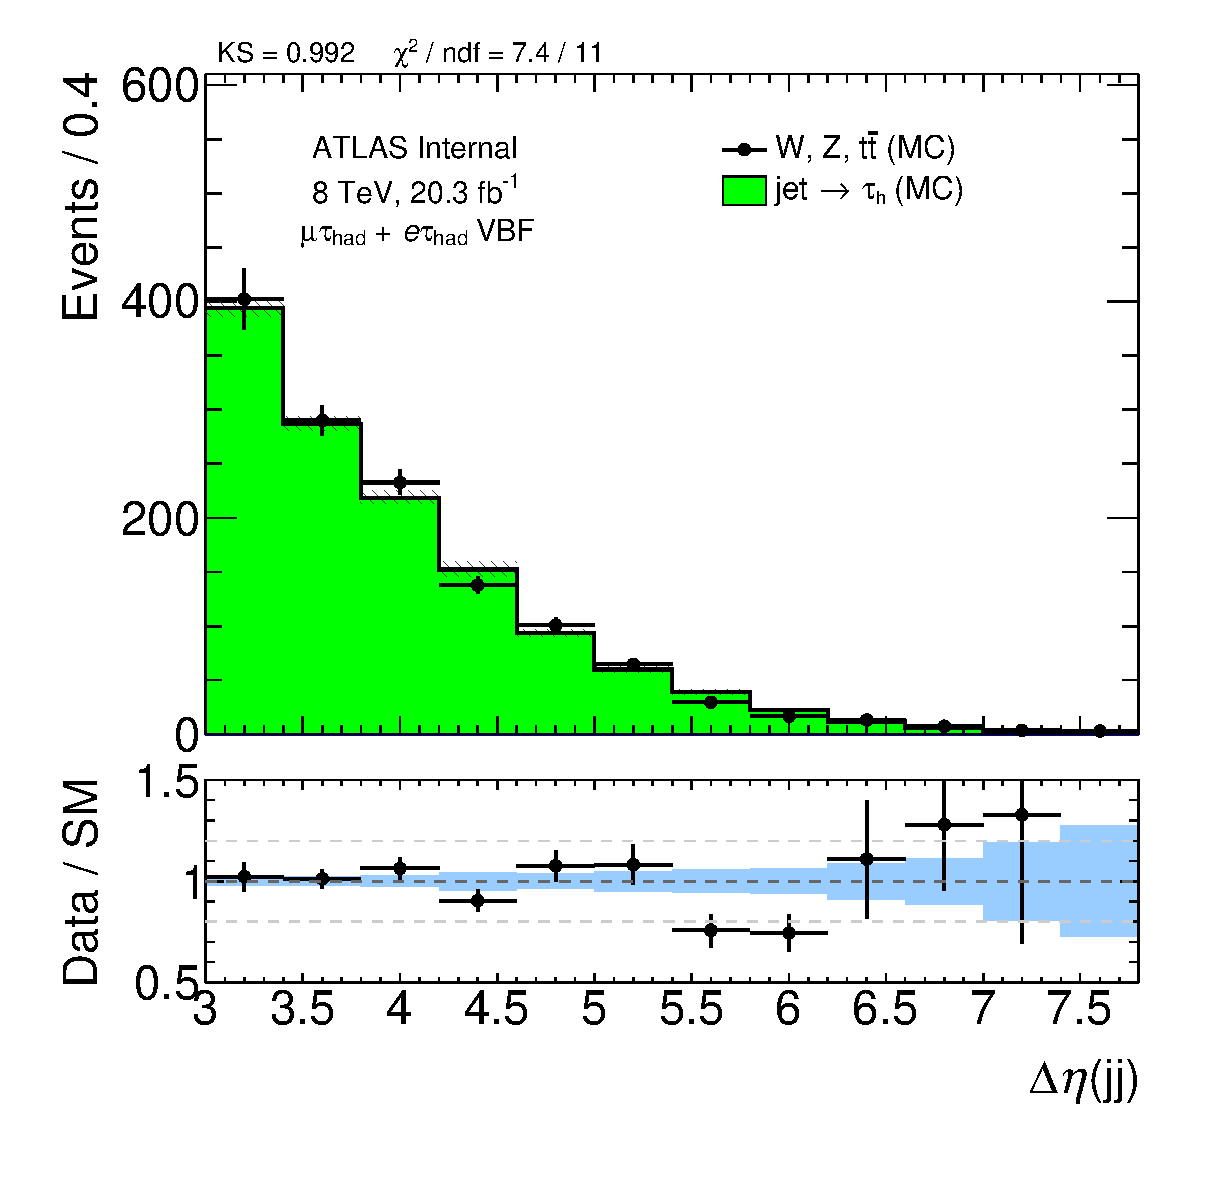
\includegraphics[width=0.32\textwidth]{figures/analysis/vbf-MCXSR/jets-deta} \\
  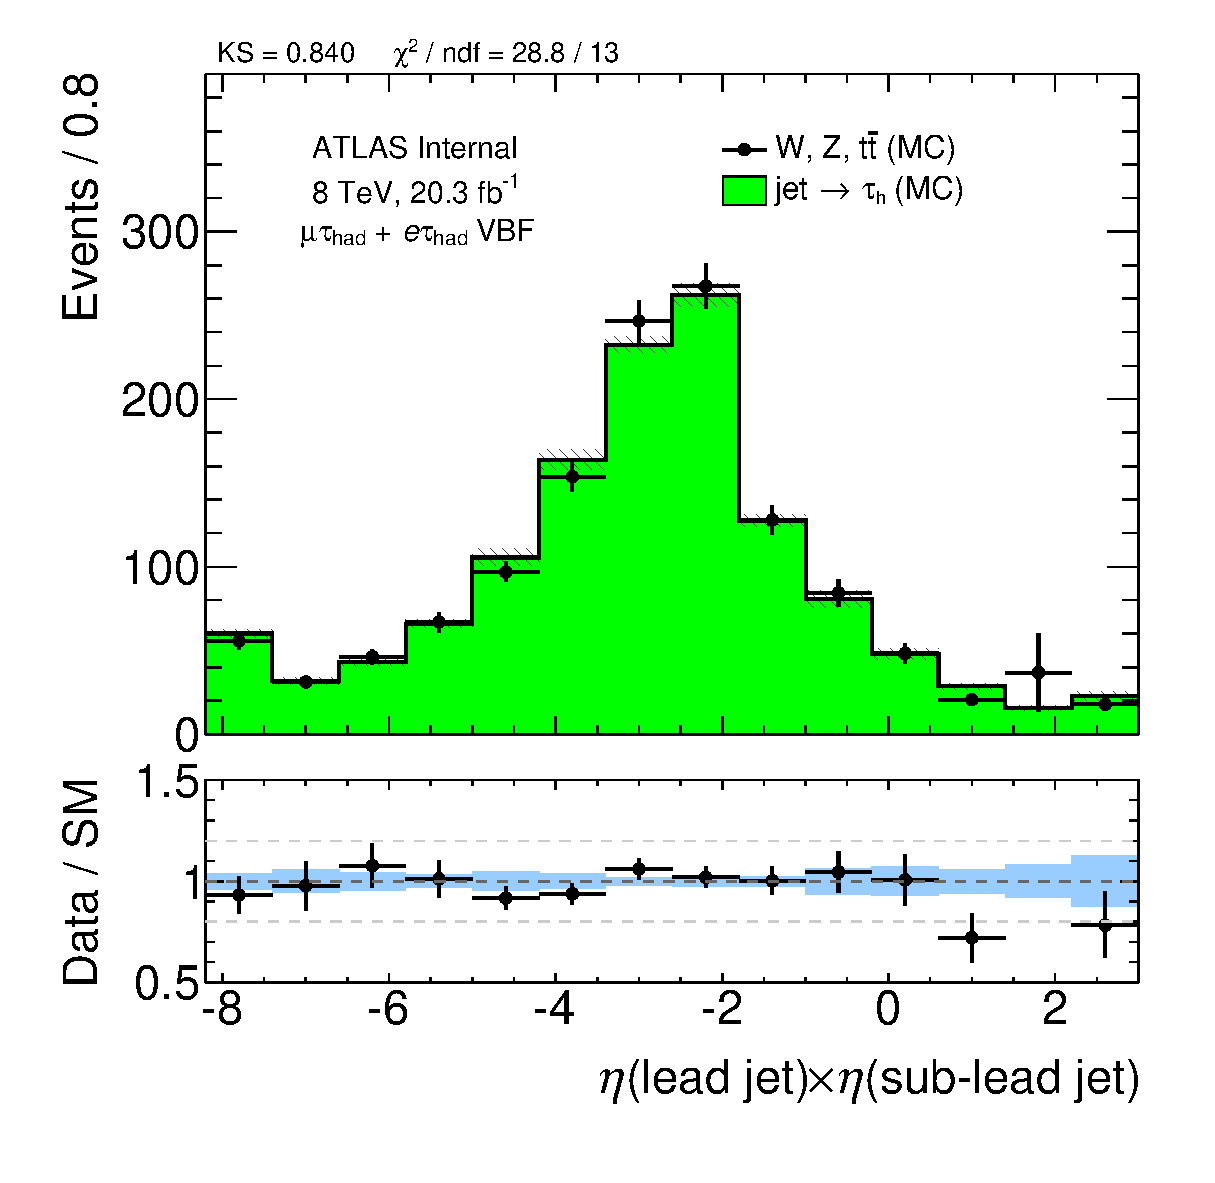
\includegraphics[width=0.32\textwidth]{figures/analysis/vbf-MCXSR/jets-etaprod} 
  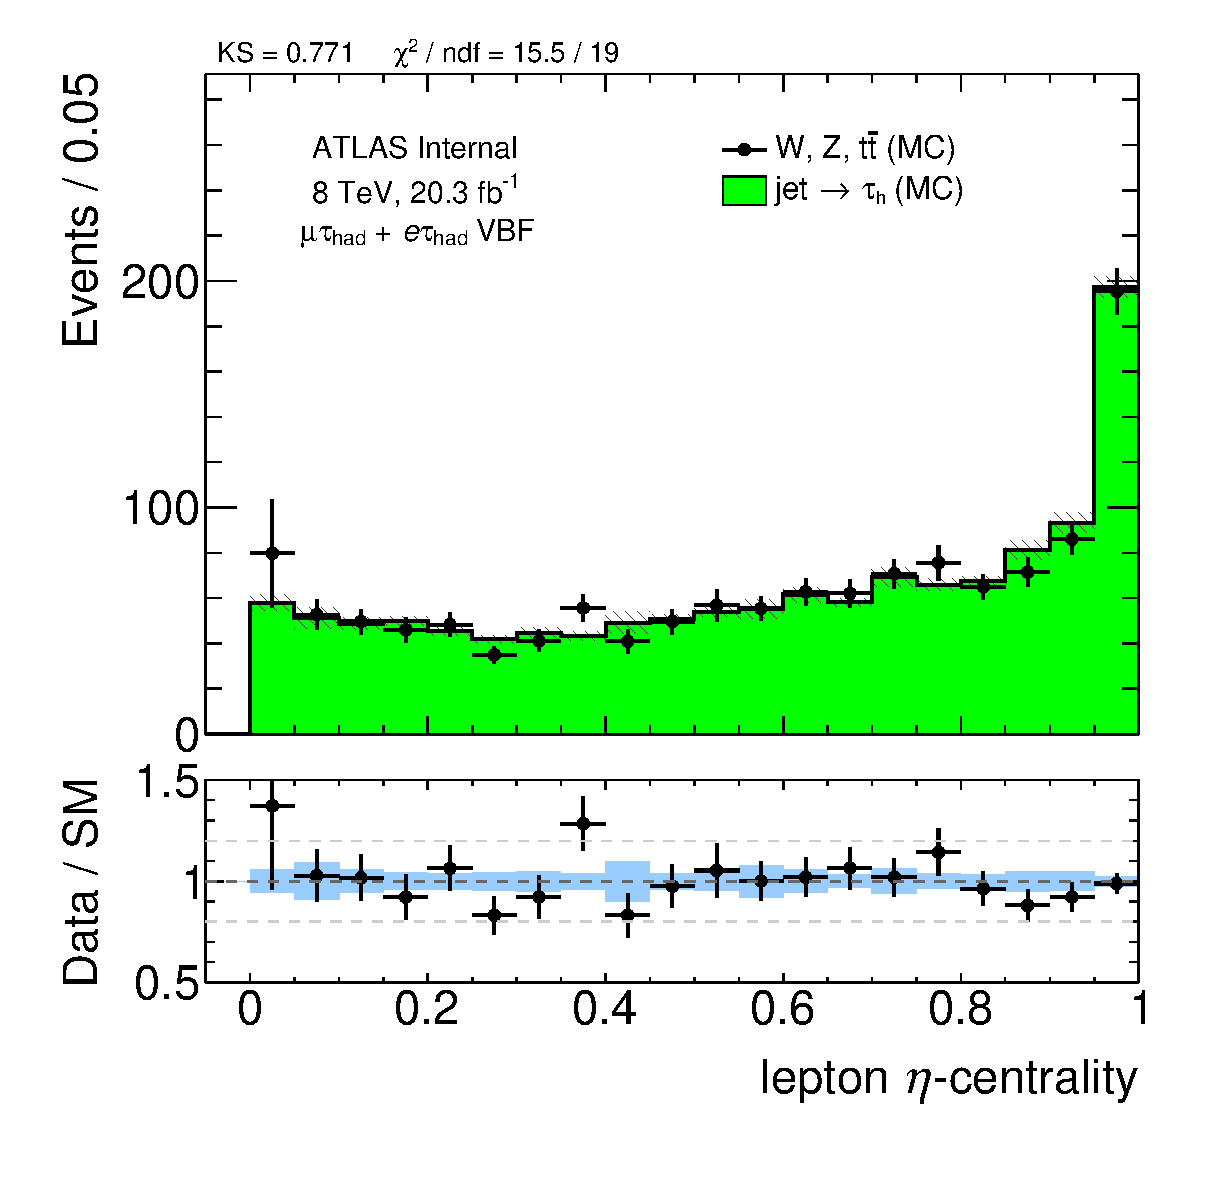
\includegraphics[width=0.32\textwidth]{figures/analysis/vbf-MCXSR/lep-eta-centrality}
  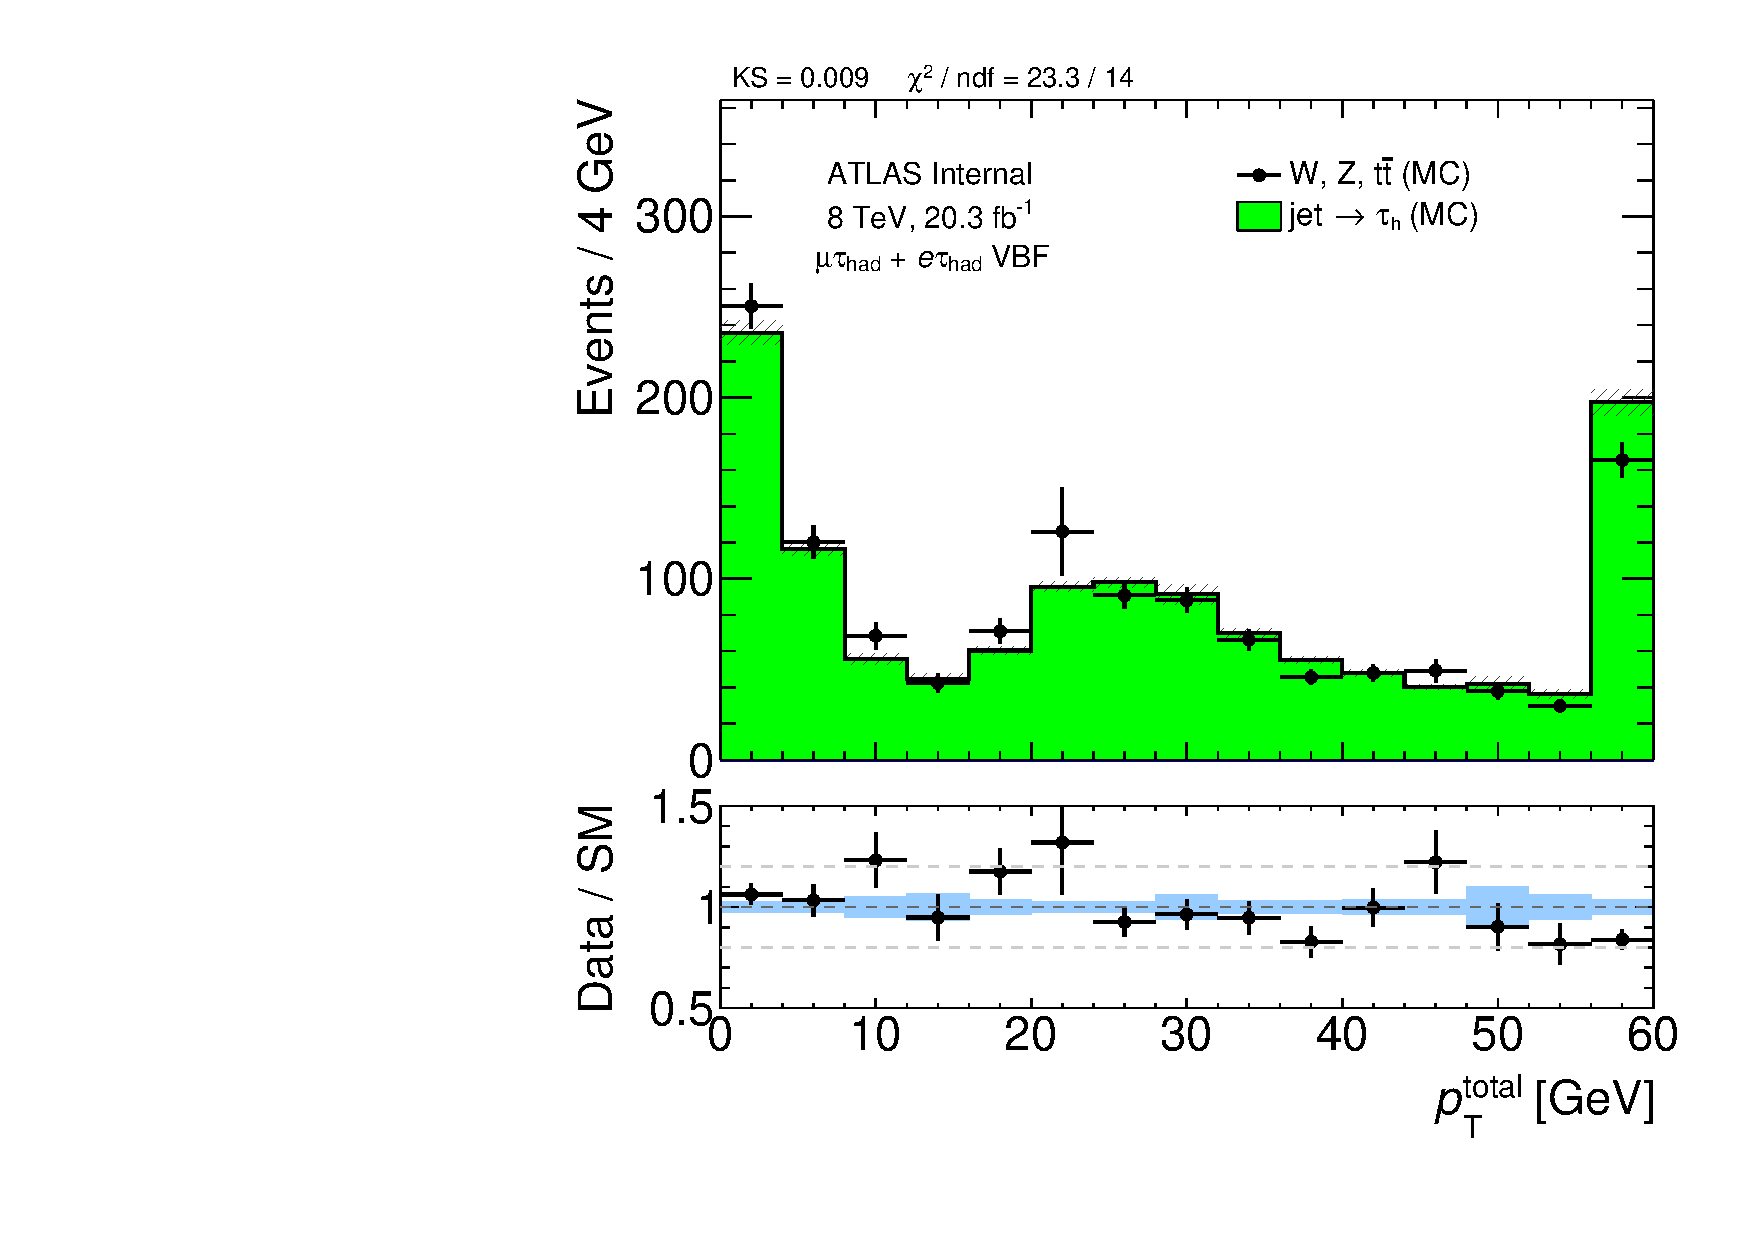
\includegraphics[width=0.32\textwidth]{figures/analysis/vbf-MCXSR/system-pt} \\
  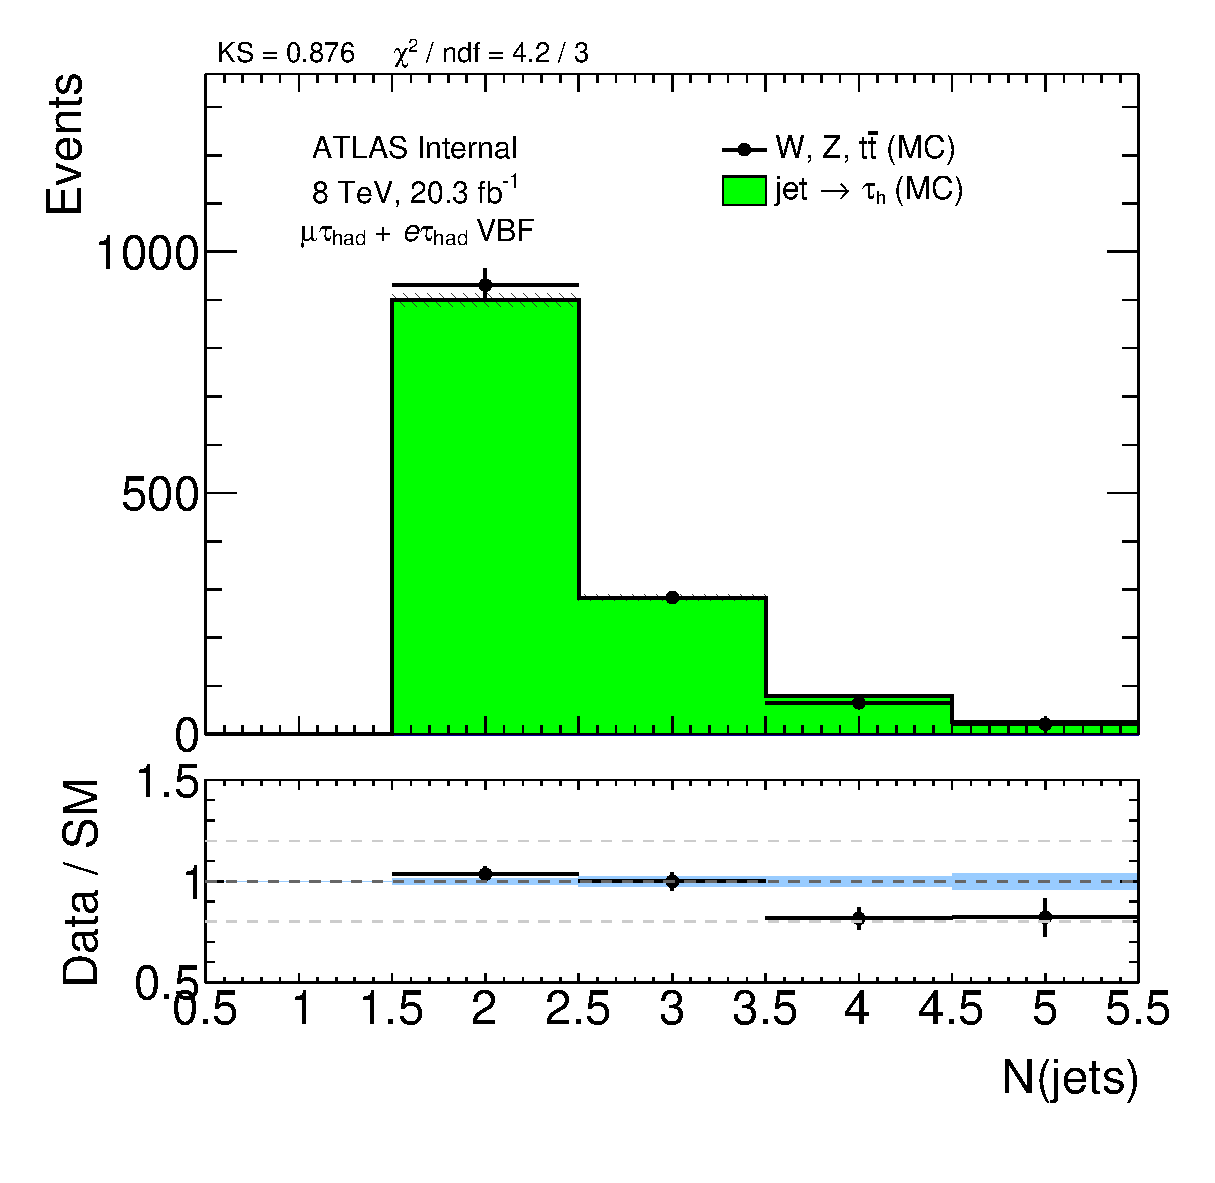
\includegraphics[width=0.32\textwidth]{figures/analysis/vbf-MCXSR/n-jets30}
  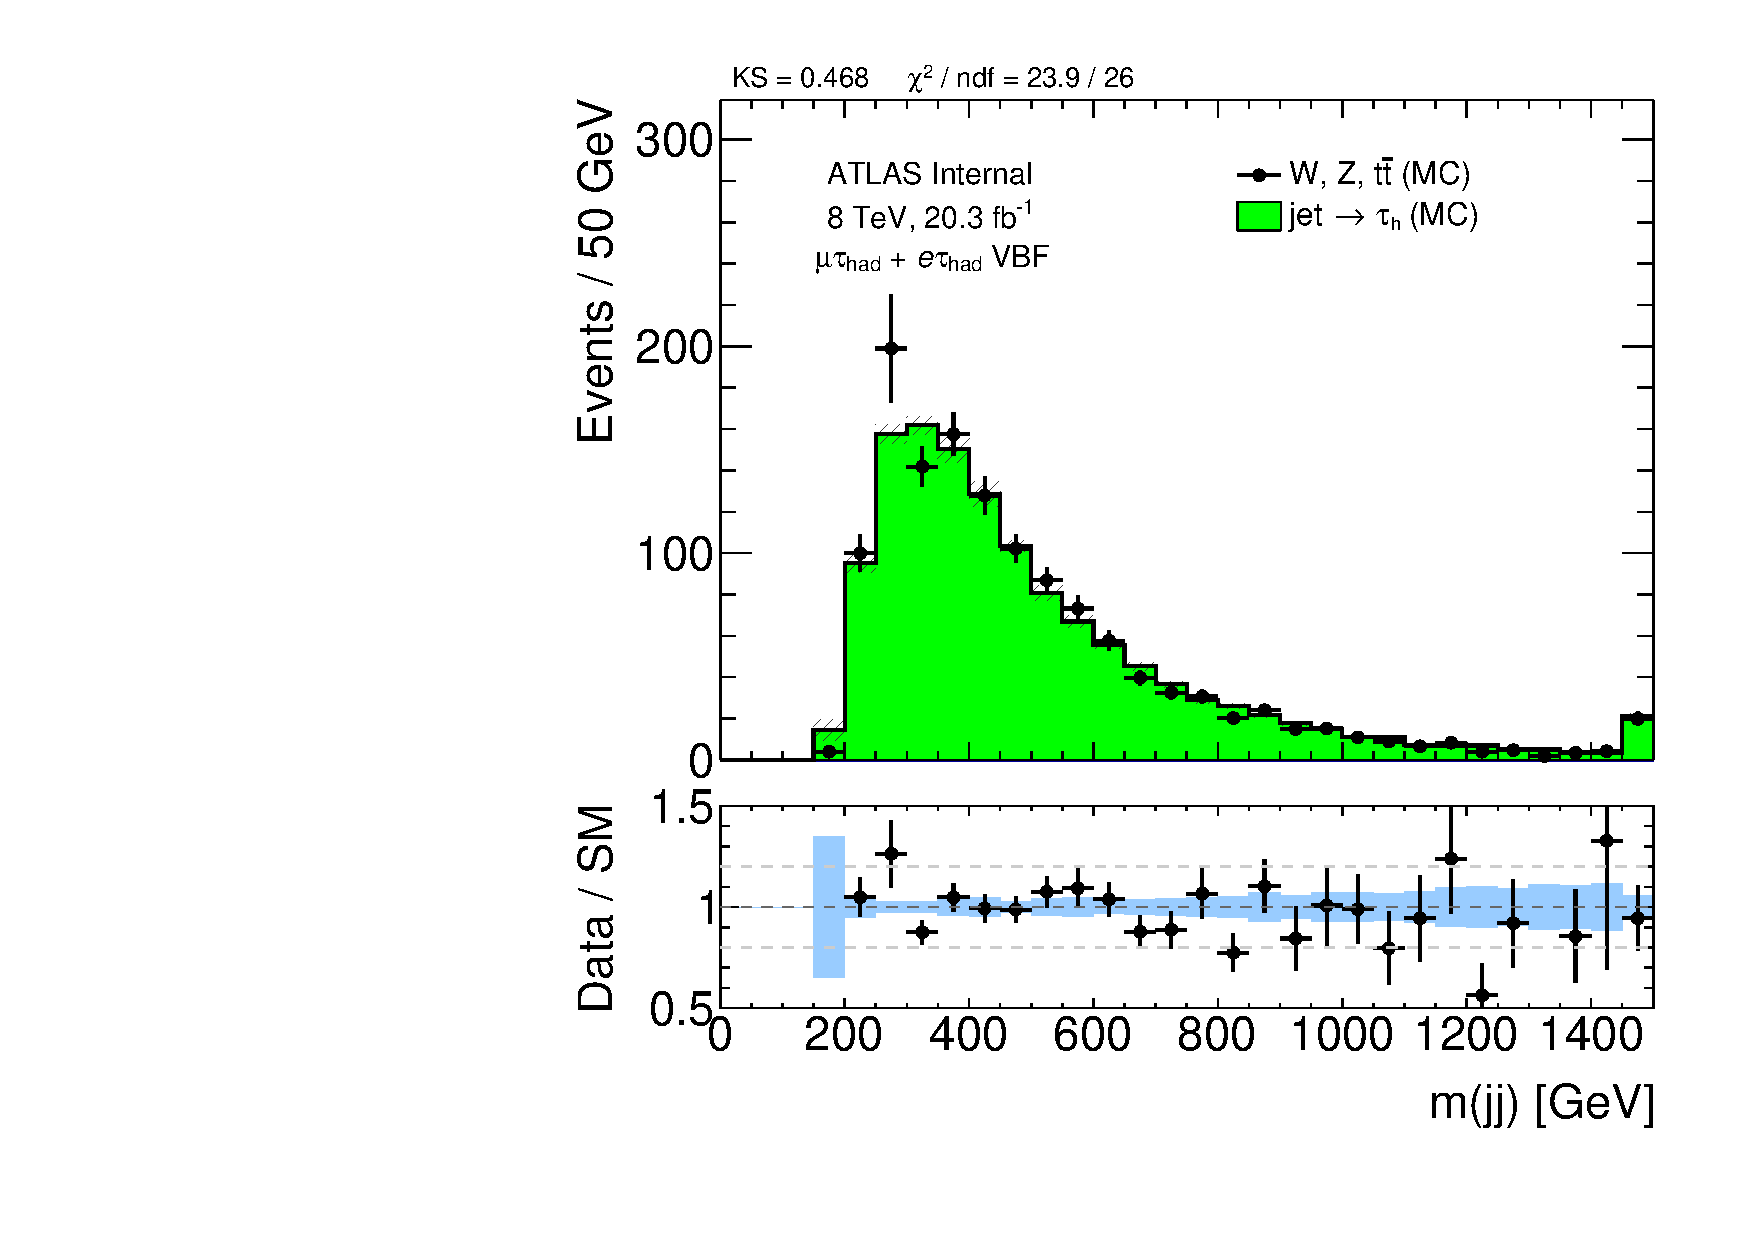
\includegraphics[width=0.32\textwidth]{figures/analysis/vbf-MCXSR/dijet-m-high}
  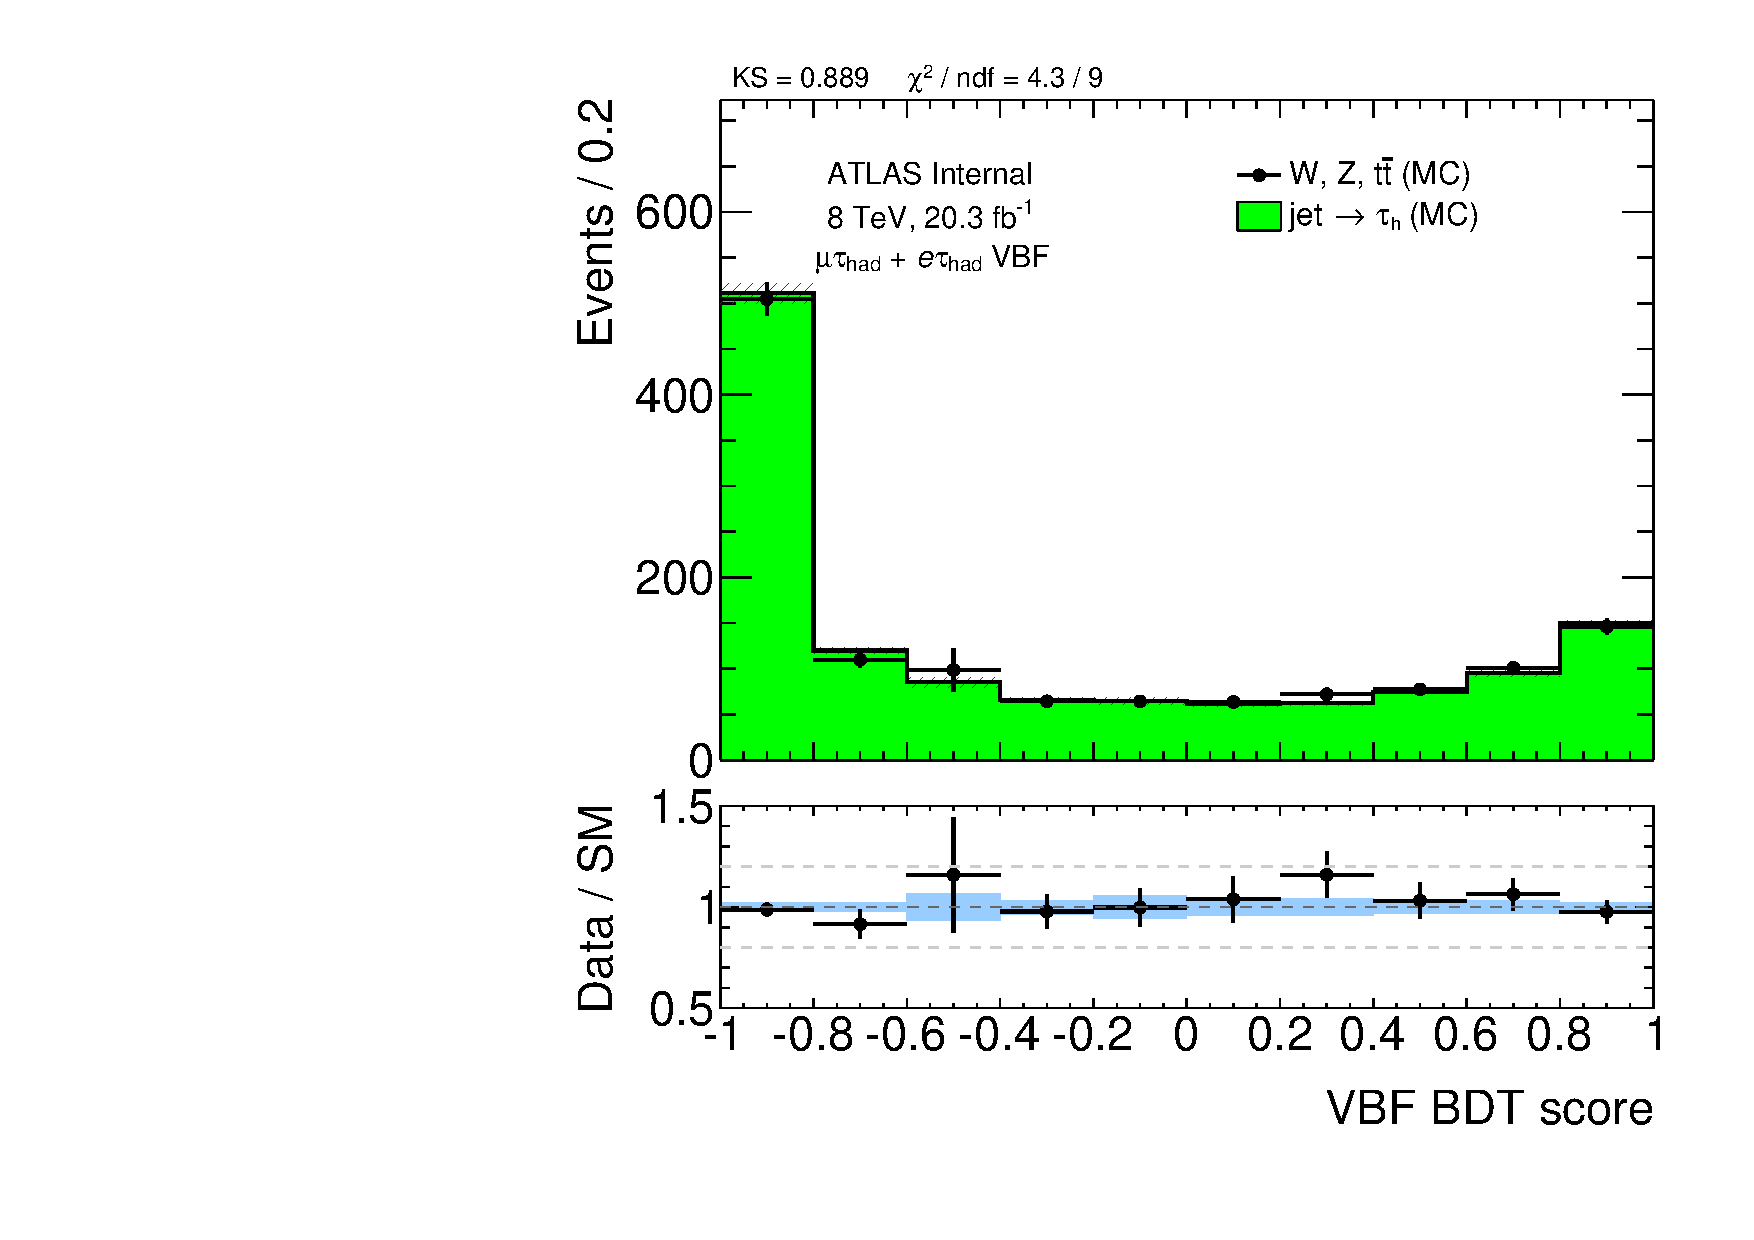
\includegraphics[width=0.32\textwidth]{figures/analysis/vbf-MCXSR/BDTEve-VBF} \\
  \caption{Comparison of the prediction of identified taus and the $\fakes$ prediction, both in simulation, in the signal region for various event kinematics. Only statistical uncertainties are shown.}
  \label{fig:backgrounds-MCXSR-jets}
\end{figure}

% \clearpage

\section{$\Wlv$ CR}

\begin{figure}[tp]
  \centering
  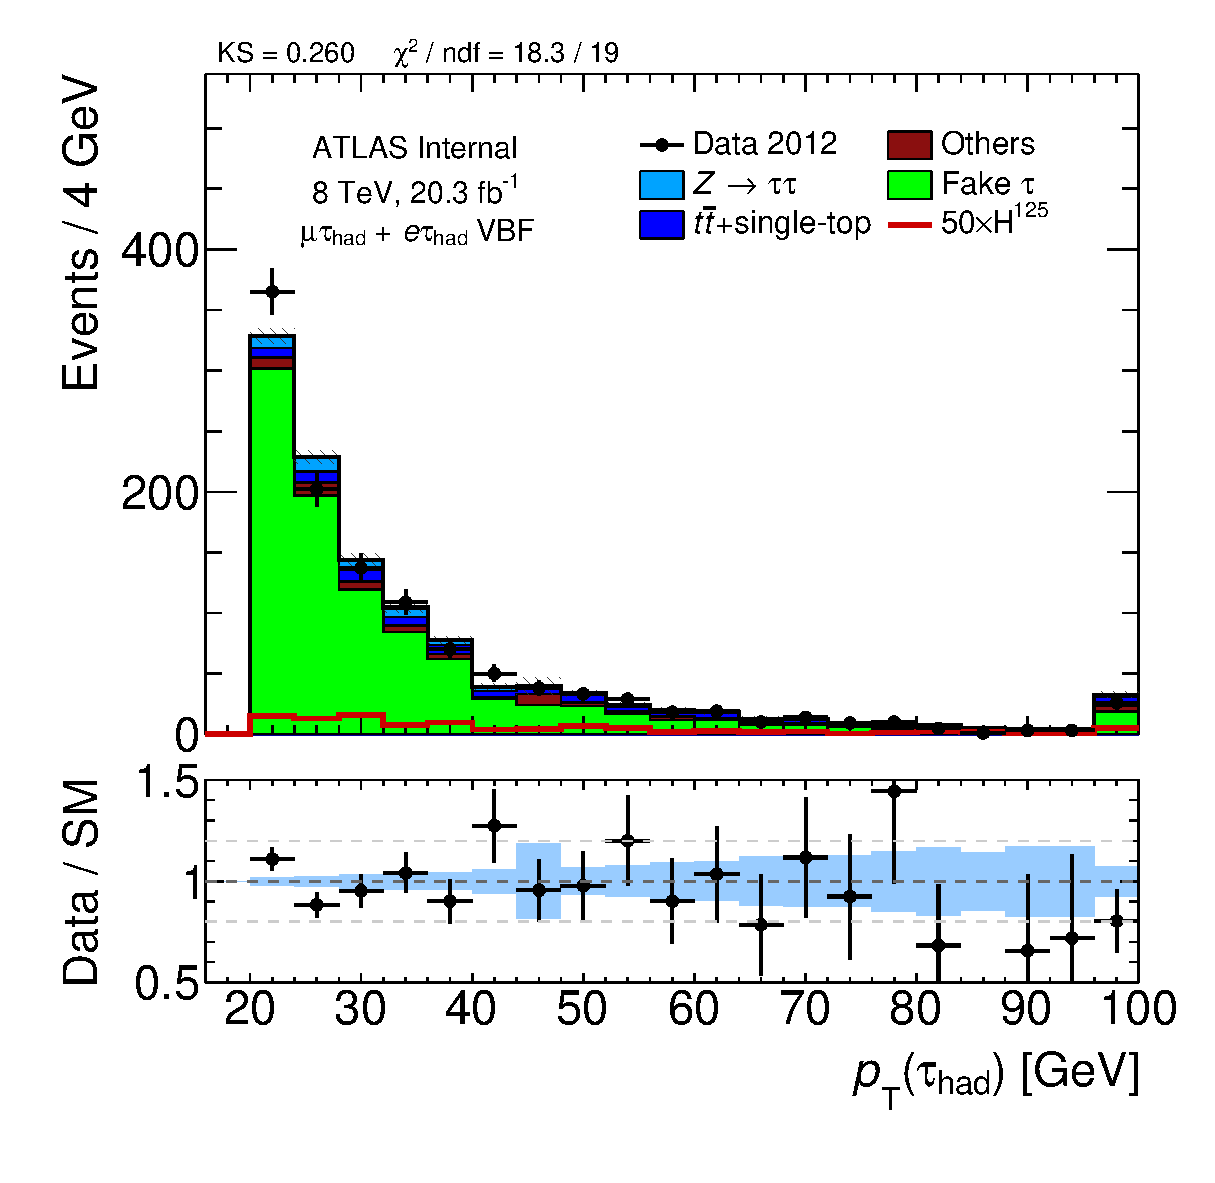
\includegraphics[width=0.32\textwidth]{figures/analysis/vbf-WlvCR/tau-pt}
  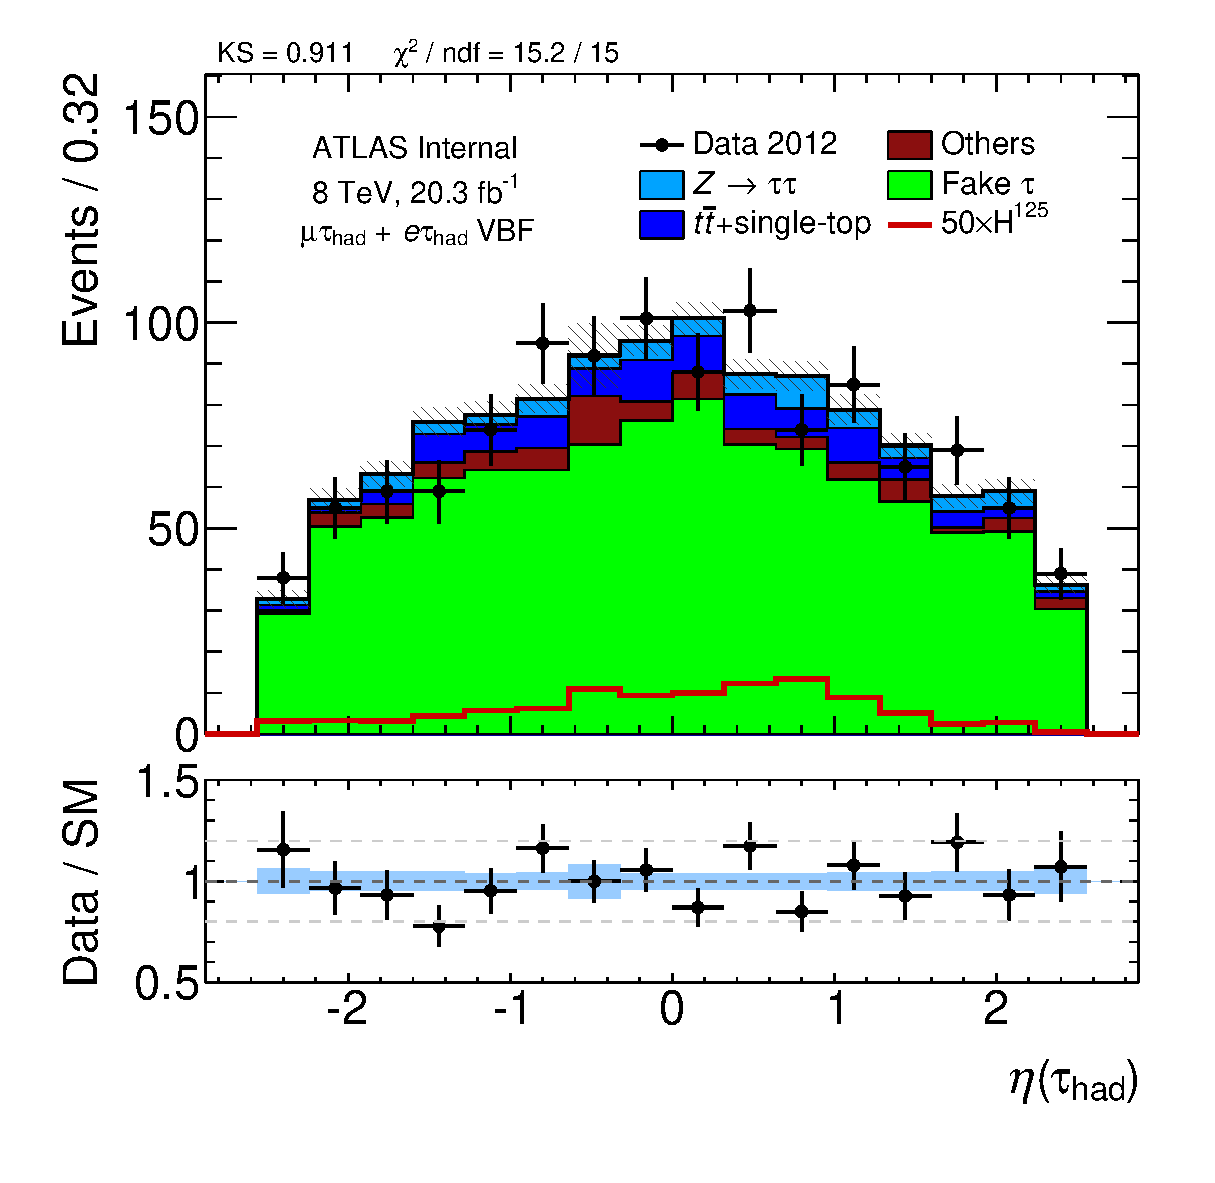
\includegraphics[width=0.32\textwidth]{figures/analysis/vbf-WlvCR/tau-eta}
  \includegraphics[width=0.32\textwidth]{figures/analysis/vbf-WlvCR/tau-numTrack} \\
  % --------------
  \includegraphics[width=0.32\textwidth]{figures/analysis/vbf-WlvCR/lep-pt-hi}
  \includegraphics[width=0.32\textwidth]{figures/analysis/vbf-WlvCR/lep-eta}
  \includegraphics[width=0.32\textwidth]{figures/analysis/vbf-WlvCR/taulep-dR} \\
  % --------------
  \includegraphics[width=0.32\textwidth]{figures/analysis/vbf-WlvCR/met-pt-hi}
  \includegraphics[width=0.32\textwidth]{figures/analysis/vbf-WlvCR/mMMC}
  \includegraphics[width=0.32\textwidth]{figures/analysis/vbf-WlvCR/mT-hi} \\
  % --------------
  \includegraphics[width=0.32\textwidth]{figures/analysis/vbf-WlvCR/met-phi-centrality}
  \includegraphics[width=0.32\textwidth]{figures/analysis/vbf-WlvCR/H-pt-hi}
  \includegraphics[width=0.32\textwidth]{figures/analysis/vbf-WlvCR/mvis} \\
  \caption{Comparison of data and $\fakes$ prediction in the $\Wlv$ CR for various event kinematics. Only statistical uncertainties are shown.}
  \label{fig:backgrounds-WlvCR-taus}
\end{figure}

\begin{figure}[tp]
  \centering
  \includegraphics[width=0.32\textwidth]{figures/analysis/vbf-WlvCR/jet-1-pt}
  \includegraphics[width=0.32\textwidth]{figures/analysis/vbf-WlvCR/jet-1-eta}
  \includegraphics[width=0.32\textwidth]{figures/analysis/vbf-WlvCR/jets-dphi} \\
  % --------------
  \includegraphics[width=0.32\textwidth]{figures/analysis/vbf-WlvCR/jet-2-pt}
  \includegraphics[width=0.32\textwidth]{figures/analysis/vbf-WlvCR/jet-2-eta}
  \includegraphics[width=0.32\textwidth]{figures/analysis/vbf-WlvCR/jets-deta} \\
  % --------------
  \includegraphics[width=0.32\textwidth]{figures/analysis/vbf-WlvCR/jets-etaprod}
  \includegraphics[width=0.32\textwidth]{figures/analysis/vbf-WlvCR/lep-eta-centrality}
  \includegraphics[width=0.32\textwidth]{figures/analysis/vbf-WlvCR/system-pt} \\
  % --------------
  \includegraphics[width=0.32\textwidth]{figures/analysis/vbf-WlvCR/n-jets30}
  \includegraphics[width=0.32\textwidth]{figures/analysis/vbf-WlvCR/dijet-m-veryhigh}
  \includegraphics[width=0.32\textwidth]{figures/analysis/vbf-WlvCR/BDTEve-VBF} \\
  \caption{Comparison of data and $\fakes$ prediction in the $\Wlv$ CR for various event kinematics. Only statistical uncertainties are shown.}
  \label{fig:backgrounds-WlvCR-jets}
\end{figure}

% \clearpage

\section{QCD CR}

\begin{figure}[tp]
  \centering
  \includegraphics[width=0.32\textwidth]{figures/analysis/vbf-QCDCR/tau-pt}
  \includegraphics[width=0.32\textwidth]{figures/analysis/vbf-QCDCR/tau-eta}
  \includegraphics[width=0.32\textwidth]{figures/analysis/vbf-QCDCR/tau-numTrack} \\
  % --------------
  \includegraphics[width=0.32\textwidth]{figures/analysis/vbf-QCDCR/lep-pt-hi}
  \includegraphics[width=0.32\textwidth]{figures/analysis/vbf-QCDCR/lep-eta}
  \includegraphics[width=0.32\textwidth]{figures/analysis/vbf-QCDCR/taulep-dR} \\
  % --------------
  \includegraphics[width=0.32\textwidth]{figures/analysis/vbf-QCDCR/met-pt-hi}
  \includegraphics[width=0.32\textwidth]{figures/analysis/vbf-QCDCR/mMMC}
  \includegraphics[width=0.32\textwidth]{figures/analysis/vbf-QCDCR/mT} \\
  % --------------
  \includegraphics[width=0.32\textwidth]{figures/analysis/vbf-QCDCR/met-phi-centrality}
  \includegraphics[width=0.32\textwidth]{figures/analysis/vbf-QCDCR/H-pt-hi}
  \includegraphics[width=0.32\textwidth]{figures/analysis/vbf-QCDCR/mvis} \\
  \caption{Comparison of data and $\fakes$ prediction in the QCD CR for various event kinematics. Only statistical uncertainties are shown.}
  \label{fig:backgrounds-QCDCR-taus}
\end{figure}

\begin{figure}[tp]
  \centering
  \includegraphics[width=0.32\textwidth]{figures/analysis/vbf-QCDCR/jet-1-pt}
  \includegraphics[width=0.32\textwidth]{figures/analysis/vbf-QCDCR/jet-1-eta}
  \includegraphics[width=0.32\textwidth]{figures/analysis/vbf-QCDCR/jets-dphi} \\
  % --------------
  \includegraphics[width=0.32\textwidth]{figures/analysis/vbf-QCDCR/jet-2-pt}
  \includegraphics[width=0.32\textwidth]{figures/analysis/vbf-QCDCR/jet-2-eta}
  \includegraphics[width=0.32\textwidth]{figures/analysis/vbf-QCDCR/jets-deta} \\
  % --------------
  \includegraphics[width=0.32\textwidth]{figures/analysis/vbf-QCDCR/jets-etaprod}
  \includegraphics[width=0.32\textwidth]{figures/analysis/vbf-QCDCR/lep-eta-centrality}
  \includegraphics[width=0.32\textwidth]{figures/analysis/vbf-QCDCR/system-pt} \\
  % --------------
  \includegraphics[width=0.32\textwidth]{figures/analysis/vbf-QCDCR/n-jets30}
  \includegraphics[width=0.32\textwidth]{figures/analysis/vbf-QCDCR/dijet-m-veryhigh}
  \includegraphics[width=0.32\textwidth]{figures/analysis/vbf-QCDCR/BDTEve-VBF} \\
  \caption{Comparison of data and $\fakes$ prediction in the QCD CR for various event kinematics. Only statistical uncertainties are shown.}
  \label{fig:backgrounds-QCDCR-jets}
\end{figure}

% \clearpage

\section{$\Zll$ CR}

\begin{figure}[tp]
  \centering
  \includegraphics[width=0.32\textwidth]{figures/analysis/vbf-ZllCR/tau-pt}
  \includegraphics[width=0.32\textwidth]{figures/analysis/vbf-ZllCR/tau-eta}
  \includegraphics[width=0.32\textwidth]{figures/analysis/vbf-ZllCR/tau-numTrack} \\
  % --------------
  \includegraphics[width=0.32\textwidth]{figures/analysis/vbf-ZllCR/lep-pt-hi}
  \includegraphics[width=0.32\textwidth]{figures/analysis/vbf-ZllCR/lep-eta}
  \includegraphics[width=0.32\textwidth]{figures/analysis/vbf-ZllCR/taulep-dR} \\
  % --------------
  \includegraphics[width=0.32\textwidth]{figures/analysis/vbf-ZllCR/met-pt-hi}
  \includegraphics[width=0.32\textwidth]{figures/analysis/vbf-ZllCR/mMMC}
  \includegraphics[width=0.32\textwidth]{figures/analysis/vbf-ZllCR/mT-hi} \\
  % --------------
  \includegraphics[width=0.32\textwidth]{figures/analysis/vbf-ZllCR/met-phi-centrality}
  \includegraphics[width=0.32\textwidth]{figures/analysis/vbf-ZllCR/H-pt-hi}
  \includegraphics[width=0.32\textwidth]{figures/analysis/vbf-ZllCR/mvis} \\
  \caption{Comparison of data and $\fakes$ prediction in the $\Zll$ CR for various event kinematics. Only statistical uncertainties are shown.}
  \label{fig:backgrounds-ZllCR-taus}
\end{figure}

\begin{figure}[tp]
  \centering
  \includegraphics[width=0.32\textwidth]{figures/analysis/vbf-ZllCR/jet-1-pt}
  \includegraphics[width=0.32\textwidth]{figures/analysis/vbf-ZllCR/jet-1-eta}
  \includegraphics[width=0.32\textwidth]{figures/analysis/vbf-ZllCR/jets-dphi} \\
  % --------------
  \includegraphics[width=0.32\textwidth]{figures/analysis/vbf-ZllCR/jet-2-pt}
  \includegraphics[width=0.32\textwidth]{figures/analysis/vbf-ZllCR/jet-2-eta}
  \includegraphics[width=0.32\textwidth]{figures/analysis/vbf-ZllCR/jets-deta} \\
  % --------------
  \includegraphics[width=0.32\textwidth]{figures/analysis/vbf-ZllCR/jets-etaprod}
  \includegraphics[width=0.32\textwidth]{figures/analysis/vbf-ZllCR/lep-eta-centrality}
  \includegraphics[width=0.32\textwidth]{figures/analysis/vbf-ZllCR/system-pt} \\
  % --------------
  \includegraphics[width=0.32\textwidth]{figures/analysis/vbf-ZllCR/n-jets30}
  \includegraphics[width=0.32\textwidth]{figures/analysis/vbf-ZllCR/dijet-m-veryhigh}
  \includegraphics[width=0.32\textwidth]{figures/analysis/vbf-ZllCR/BDTEve-VBF} \\
  \caption{Comparison of data and $\fakes$ prediction in the $\Zll$ CR for various event kinematics. Only statistical uncertainties are shown.}
  \label{fig:backgrounds-ZllCR-jets}
\end{figure}

% \clearpage

\section{top CR}

\begin{figure}[tp]
  \centering
  \includegraphics[width=0.32\textwidth]{figures/analysis/vbf-topCR/tau-pt}
  \includegraphics[width=0.32\textwidth]{figures/analysis/vbf-topCR/tau-eta}
  \includegraphics[width=0.32\textwidth]{figures/analysis/vbf-topCR/tau-numTrack} \\
  % --------------
  \includegraphics[width=0.32\textwidth]{figures/analysis/vbf-topCR/lep-pt-hi}
  \includegraphics[width=0.32\textwidth]{figures/analysis/vbf-topCR/lep-eta}
  \includegraphics[width=0.32\textwidth]{figures/analysis/vbf-topCR/taulep-dR} \\
  % --------------
  \includegraphics[width=0.32\textwidth]{figures/analysis/vbf-topCR/met-pt-hi}
  \includegraphics[width=0.32\textwidth]{figures/analysis/vbf-topCR/mMMC}
  \includegraphics[width=0.32\textwidth]{figures/analysis/vbf-topCR/mT} \\
  % --------------
  \includegraphics[width=0.32\textwidth]{figures/analysis/vbf-topCR/met-phi-centrality}
  \includegraphics[width=0.32\textwidth]{figures/analysis/vbf-topCR/H-pt-hi}
  \includegraphics[width=0.32\textwidth]{figures/analysis/vbf-topCR/mvis} \\
  \caption{Comparison of data and $\fakes$ prediction in the top CR for various event kinematics. Only statistical uncertainties are shown.}
  \label{fig:backgrounds-topCR-taus}
\end{figure}

\begin{figure}[tp]
  \centering
  \includegraphics[width=0.32\textwidth]{figures/analysis/vbf-topCR/jet-1-pt}
  \includegraphics[width=0.32\textwidth]{figures/analysis/vbf-topCR/jet-1-eta}
  \includegraphics[width=0.32\textwidth]{figures/analysis/vbf-topCR/jets-dphi} \\
  % --------------
  \includegraphics[width=0.32\textwidth]{figures/analysis/vbf-topCR/jet-2-pt}
  \includegraphics[width=0.32\textwidth]{figures/analysis/vbf-topCR/jet-2-eta}
  \includegraphics[width=0.32\textwidth]{figures/analysis/vbf-topCR/jets-deta} \\
  % --------------
  \includegraphics[width=0.32\textwidth]{figures/analysis/vbf-topCR/jets-etaprod}
  \includegraphics[width=0.32\textwidth]{figures/analysis/vbf-topCR/lep-eta-centrality}
  \includegraphics[width=0.32\textwidth]{figures/analysis/vbf-topCR/system-pt} \\
  % --------------
  \includegraphics[width=0.32\textwidth]{figures/analysis/vbf-topCR/n-jets30}
  \includegraphics[width=0.32\textwidth]{figures/analysis/vbf-topCR/dijet-m-veryhigh}
  \includegraphics[width=0.32\textwidth]{figures/analysis/vbf-topCR/BDTEve-VBF} \\
  \caption{Comparison of data and $\fakes$ prediction in the top CR for various event kinematics. Only statistical uncertainties are shown.}
  \label{fig:backgrounds-topCR-jets}
\end{figure}


